\documentclass[german,a4paper,12pt,oneside]{article}

\usepackage{definitions}
\usepackage{packages}

\renewcommand{\abstractname}{Zusammenfassung}

\captionsetup[table]{labelfont=bf}
\captionsetup[figure]{labelfont=bf}
\graphicspath{{./images/}}

\renewcommand\labelitemi{$\vcenter{\hbox{\tiny$\bullet$}}$}

\makenomenclature
\renewcommand\nompreamble{\begin{multicols}{2}}
\renewcommand\nompostamble{\end{multicols}}

\begin{document}

\begin{titlepage}
    \sf

    \newsavebox{\textblock}
    \savebox{\textblock}{%
    \begin{tabular}{@{}l@{}}
        Technische Universit\"at M\"unchen \\
        TUM School of Computation, Information and Technology \\
        Department of Mathematics
    \end{tabular}
    }

    \newlength{\textblockheight}
    \setlength{\textblockheight}{\ht\textblock}

    \noindent
    \begin{minipage}{\textwidth}
    \usebox{\textblock}%
    \hfill
    \raisebox{-15pt}[0pt][0pt]{
        
\includegraphics[height=1.35cm]{Jonas_TUM_schwarz.png}%
    }
    \end{minipage}

    \begin{center}
        
        \vspace*{6.5cm}
        
        \Large
        A thesis presented for the degree of \\
        Bachelor of Science of Mathematics

        \vspace*{0.8cm}
        
        \Large
        \textbf{From Solar Geometry to Direct Current Output: A Mathematical Approach to Photovoltaic System Modeling} 
            
        \vspace{1cm}
        
        \Large 
        %\textbf{Leon Holtkamp}
        Leon Holtkamp

        \vspace{1.3cm}
        
        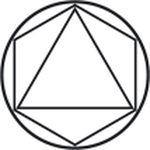
\includegraphics[scale=0.9]{Jonas_CIT_schwarz.png}
    \end{center}
    \vspace*{\fill}
    
    \noindent
    \begin{tabular}{ll}
        Supervisor: & Prof. Dr. Oliver Junge \\
        Advisor:    & Dr. Vadim Gorski         \\
        Submission: & \today
    \end{tabular}
\end{titlepage}

\newpage
    


\begin{abstract}
    Die vorliegende Arbeit bietet einen Einblick in die Modellierung
    von Photovoltaikanlagen mit dem Ziel, die erzeugte Gleichstrom-Leistung der Anlage
    für gegebene Umweltbedingungen zu simulieren. Zu diesem Zweck wird ein
    bekanntes physikalisches Modell verwendet, das die Strom-Spannungskurve
    eines einzelnen Photovoltaikmoduls in Abhängigkeit von der einfallenden
    Solarstrahlung und der Zelltemperatur beschreiben kann. Mithilfe
    praktischer Überlegungen lässt sich dieses Modell auf die Modellierung
    von Photovoltaiksystemen, bestehend aus mehreren Modulen, übertragen.
    Die benötigten Umweltparameter des Modells werden mit Hilfe von zwei
    weiteren bekannten Modellen, sogenannten Thermo- und Transpositionsmodellen,
    aus meteorologischen Daten abgeleitet. Dabei spielt das Wissen über
    die Modellierung der Solarstrahlung auf geneigte Flächen eine zentrale
    Rolle, worauf zu Beginn der Arbeit eingegangen wird.
    Des Weiteren werden alle Gleichungen und Berechnungsmethoden, die bei der
    Bestimmung der Modellparameter zum Einsatz kommen, umfassend beschrieben, sodass
    das Modell auf verschiedene Arten von Photovoltaikmodulen angewendet werden
    kann. Abschließend wird das Modell genutzt, um die Stromproduktion einer
    4,62 kWh Photovoltaikanlage in Bayern, Deutschland, zu simulieren.
    Die benötigten Wetterdaten wurden von nahegelegenen Wetterstationen des
    Deutschen Wetterdienstes bezogen. Die Analyse der Ergebnisse zeigt,
    dass die Genauigkeit des Modells erheblich von der Qualität der verwendeten
    Wetterdaten abhängt. In Zeiträumen, in denen die Abweichung zwischen den
    gemessenen und tatsächlichen Umweltbedingungen mit großer Sicherheit gering ist,
    zeigte das Modell eine hohe Genauigkeit.
\end{abstract}

\newpage

\vspace*{\fill}

\noindent
I hereby declare that I have prepared this thesis independently and only with the specified aids.

\vspace{2cm}
\noindent
Erding, \today, 

\vspace{0.5cm}
\newpage

\tableofcontents
\newpage

\section{Introduction}

The impact of human activities on Earth's climate has been unequivocally demonstrated
by scientists over the past decade. In response, global leaders have adopted common 
environmental goals to protect the planet. Consequently, the global energy production mix
has shifted significantly towards green energy. Given the inherently complex nature of
renewables, extensive research across various disciplines has been conducted to improve and 
understand emerging technologies. Solar energy stands out as one of the most important energy
resources for humanity, being clean, pollution-free and inexhaustible. Remarkably, the Earth
receives enough solar energy in a matter of hours to meet the world's energy demand of an
entire year. Advances in photovoltaic (PV) technology and reductions in manufacturing costs
have led to a multifold increase in PV capacity, often characterized by decentralized deployment
and fluctuating power output due to variable weather conditions.

Accurate modeling of PV modules is of vital importance in many fields.
It enables designers to optimize system performance and maximize cost-effectiveness.
Power forecasts support grid operators in balancing power demand and supply, while
plant operators utilize predictions for energy management and to achieve the best economic
outcome. The challenges posed by volatile production are being addressed by battery
systems, whose optimized charging management depends on reliable generation data.

The performance of a PV module largely depends on the availability of solar 
radiation and its conversion efficiency. These aspects are influenced by numerous
physical parameters, including the geographical location of the
site, panel orientation, weather conditions, surrounding obstructions,
the electrical load etc. \cite[p. 1358f]{LoBrano}. Unsurprisingly, energy assessments
based on simplistic models that assume a constant value for the conversion
efficiency can yield erroneously optimistic predictions \cite{Wang2021}.
Unfortunately, the information provided by the manufacturers often lacks the detail
needed to exploit high-performance predictive tools. An analysis of information
from over 400 manufacturers' websites revealed that the quality of this information is variable,
sometimes inconsistent, and often inadequate for reliable designs \cite[p. 1161]{Orioli}.

The variability of available manufacturing, meteorological and site-related data
resulted in a wide spectrum of forecasting models, broadly classified
into three main categories: physical, statistical and hybrid \cite{Ulbricht2013, Iheanetu2022}. 
Physical models simulate the conversion of solar irradiation into electricity
using physical equations. The more complex spectrum of these models can accurately describe
the behavior of PV modules when high-quality input and calibration data are available.
In contrast, statistical models aim to establish the relationship between input
variables and the corresponding power output without relying on physical equations.
Many statistical models require prior training on historical meteorological
and generation datasets, where training involves calculating model parameters
through mathematical optimization methods that accurately represent the
relationship between the datasets and can generalize to unseen data.
As might be expected, physical and statistical models can be combined to
create hybrid models. Such combinations may overcome individual drawbacks
and further improve accuracy, albeit with the potential downside of increased
complexity and greater computational resource requirements.

This thesis introduces an approach to predict the direct current
(DC) power output of a PV system of arbitrary size and configuration under
certain assumptions. A well-known five-parameter physical model
builds the basis of this approach, which can be calibrated with a
minimal set of data provided by manufacturers. Required meteorological
parameters include temperature, wind speed, air pressure as well as global
and diffuse horizontal radiation. The model also requires the geographical
location of the PV system and the orientation of the individual PV arrays in
order to estimate the input variables for the physical model. The 
presented approach can be combined with a conversion model to predict
the generated alternating current (AC) power required for load consumption
and connection to the electrical grid.

This thesis is structured as follows: Chapter \ref{sec:Solar Geometry and Radiation}
introduces the basics of solar geometry and solar radiation. Chapter 
\ref{sec:Photovoltaic system modeling and power prediction} details
the physical modeling of PV systems and introduces the five-parameter model.
In Chapter \ref{sec:Application and analysis of the model}, the presented model is
applied to a 4.62 kW PV system and analyzed. Finally, Chapter \ref{sec:Conclusion}
concludes the thesis and outlines potential directions for future work.

\newpage

\section{Solar geometry and radiation}
A key input variable for the physical model presented in this thesis
is the irradiance received by an arbitrarily oriented surface on Earth.
Estimating this variable from global horizontal and diffuse horizontal
irradiance data relies on a transposition model. The
formulation of this model requires a solid understanding of the
Sun's position relative to Earth's surface
and oriented planes, as well as foundational knowledge of solar
radiation modeling. The following sections cover these basic concepts
and introduce a well-known transposition model used in this
thesis at the end of this chapter.

\label{sec:Solar Geometry and Radiation}
\subsection{Solar geometry and sun position}

The position of the Sun in the sky, as observed from a given point on the Earth's surface, can be described
using two angles: the \textbf{solar altitude} \(\gamma_{\text{s}}\) and the \textbf{solar azimuth}
\(\alpha_{\text{s}}\). Let \(L\) denote the line connecting the observer's point on the Earth's surface to the
center of the solar disk and let \(\tilde{L}\) denote the projection of \(L\) onto the horizontal plane.
The solar altitude \(\gamma_{\text{s}}\) is the angle between \(L\) and \(\tilde{L}\) and the solar azimuth \(\alpha_{\text{s}}\)
is the angle between a line running in a true north-south direction and \(\tilde{L}\). In the Northern Hemisphere,
the solar azimuth angle is measured clockwise from due south, while in the Southern Hemisphere, it is measured
counterclockwise from due north. Values are negative before solar noon and positive after solar noon, corresponding
to positive values for directions west of the north-south line and negative values east of it \cite[p. 9]{CIBSE}.
This definition is used throughout the rest of the thesis, with the note that different conventions exist in
the literature. For example, Muneer \cite{Muneer} measures this angle positively clockwise from due north. Another important
angle is the solar zenith angle \(\psi_{\text{s}}\), which is the complement of the solar altitude angle relative to the
zenith direction, given by \(\psi_{\text{s}} = 90^\circ - \gamma_{\text{s}}\). The altitude angle is also referred to as the
elevation angle, indicating the elevation of the Sun above the horizon. Figure \ref{fig:SolarGeometry} illustrates
the solar geometry in relation to an oriented surface.

\begin{figure}
    \centering
    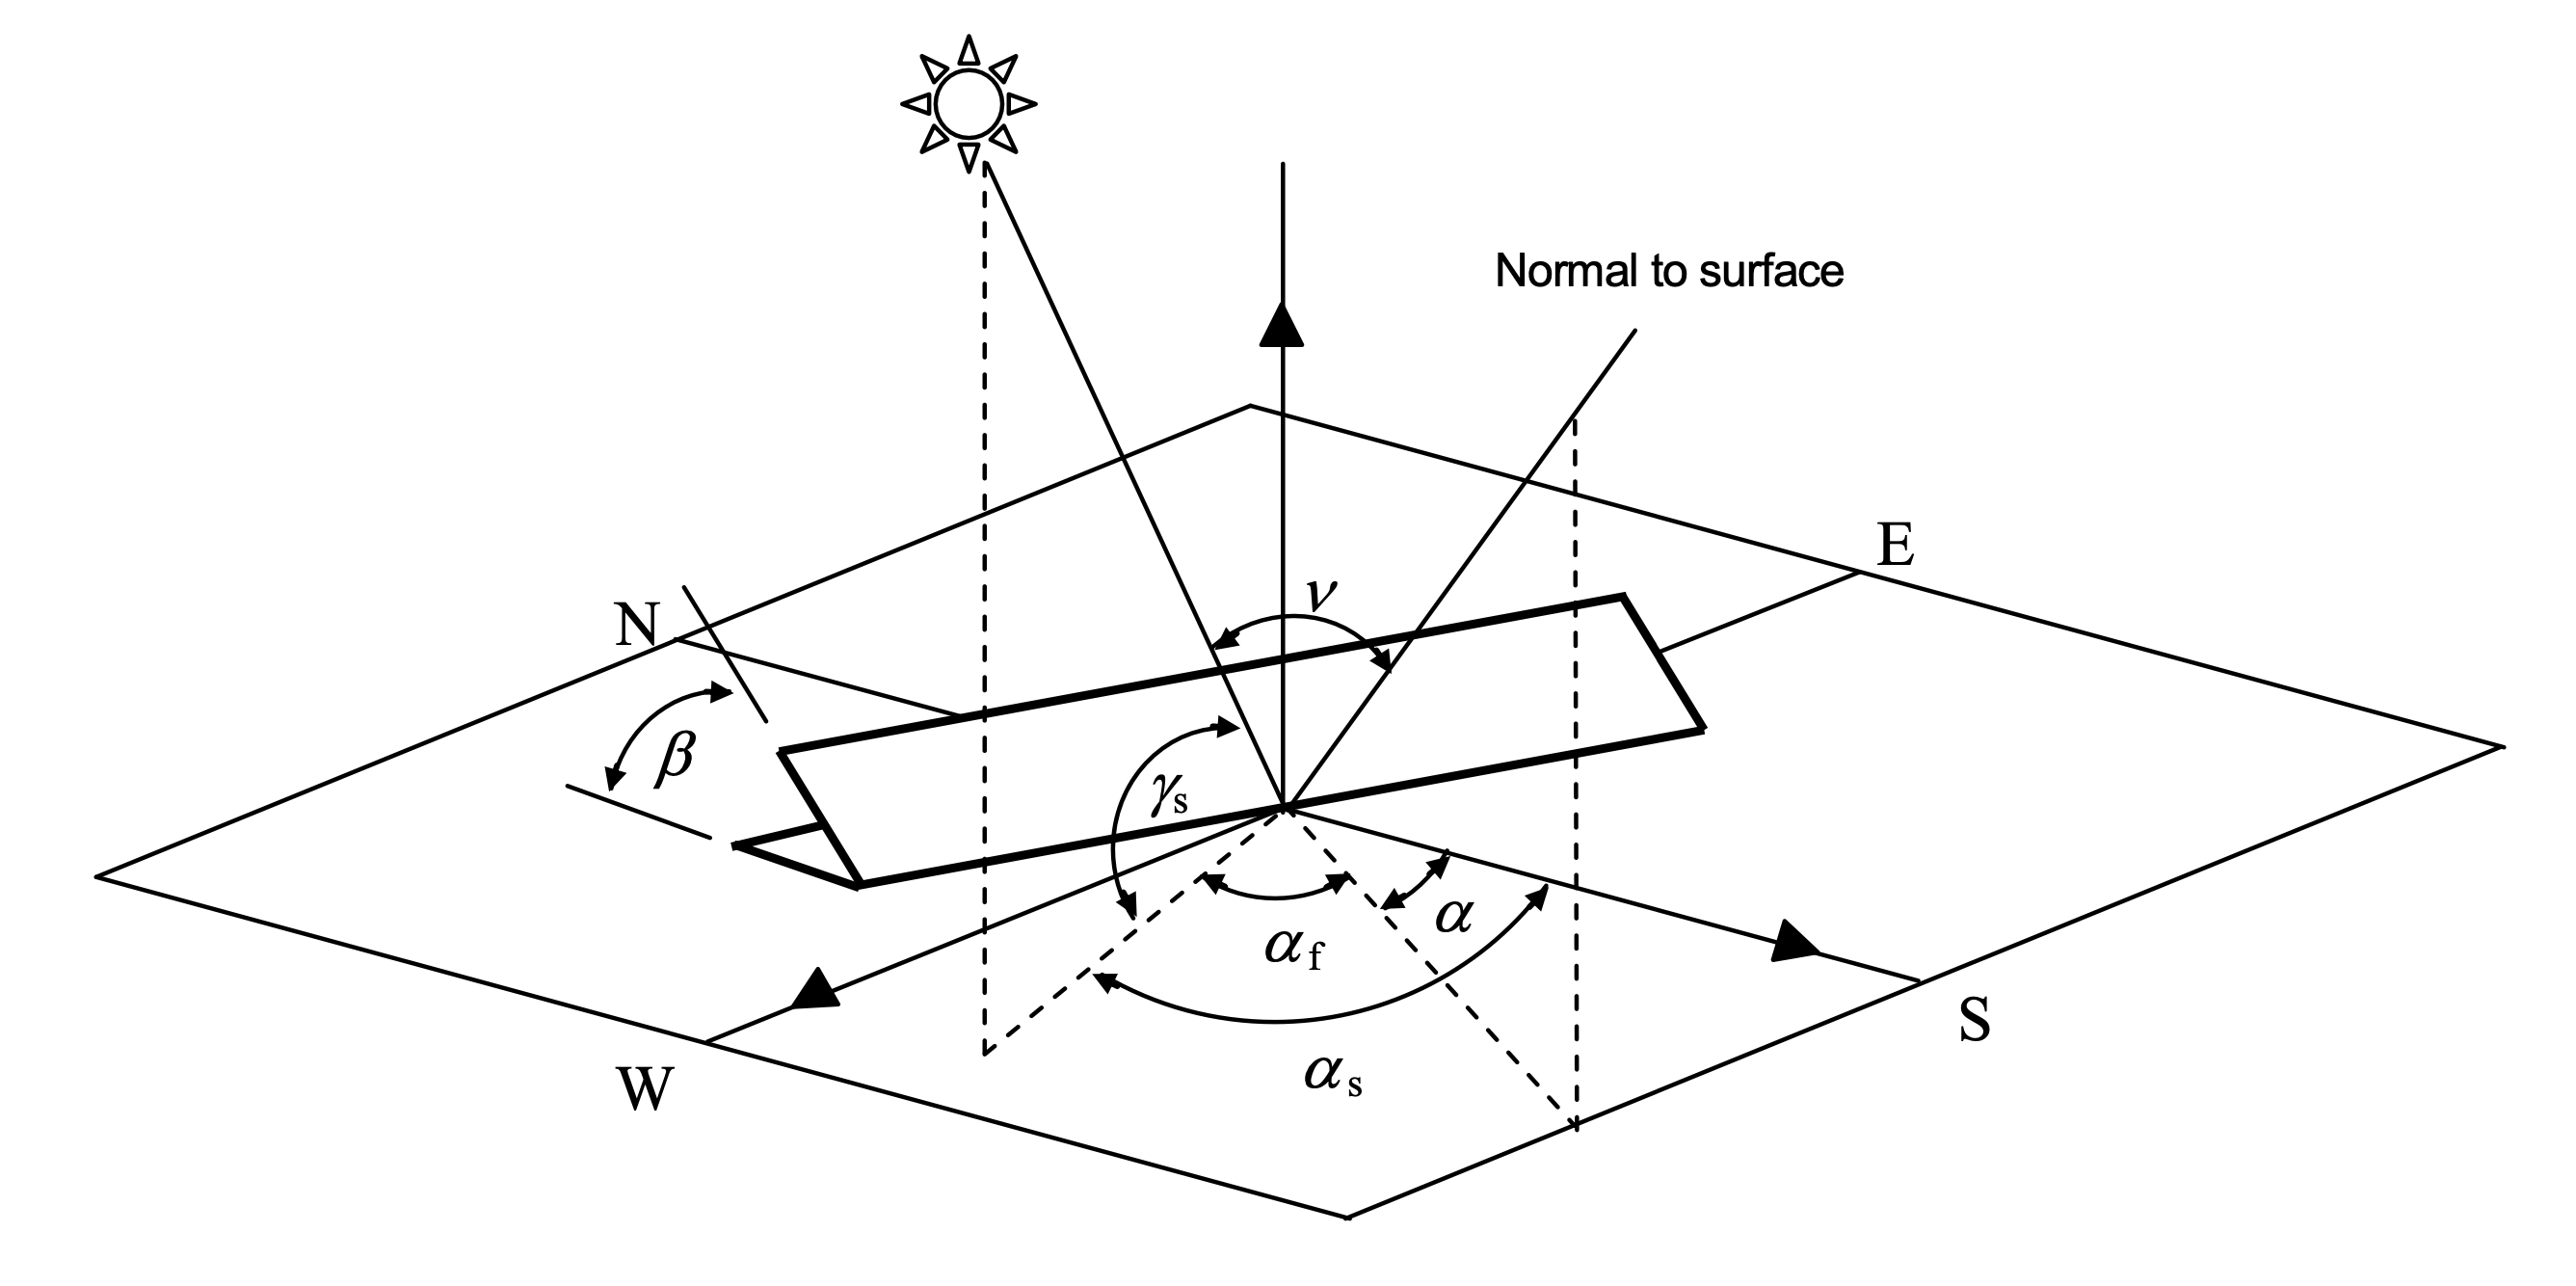
\includegraphics[scale=0.15]{Solar_Geometry_CIBSE}
    \caption{\small Solar geometry in relation to an oriented surface in the Northern Hemisphere \cite{CIBSE}.}
    \label{fig:SolarGeometry} % see https://www.overleaf.com/learn/latex/Inserting_Images
\end{figure}

As shown in the figure, the orientation of a surface can also be described using two angles: 
the surface tilt \(\beta\) and the surface azimuth \(\alpha\). The surface tilt angle \(\beta\) represents
the angular elevation of the surface from the horizontal plane, while the surface azimuth
angle \(\alpha\) describes the direction the inclined surface faces. Similar to the solar azimuth 
angle, different conventions exist in the literature. Throughout this work, the same  
convention as for the solar azimuth angle is used, as illustrated in the figure. For reference,
a selection of angle values and their interpretations is presented in Table \ref{tab:angles_and_values}.

\begin{table}
    \centering
    \begin{tabular}{rl@{\hspace{0.5cm}}rl@{\hspace{0.5cm}}rl}
        \toprule
        \multicolumn{2}{l}{\textbf{Surface tilt \(\beta\)}} & \multicolumn{2}{l}{\textbf{Solar altitude \(\gamma_{\text{s}}\)}} & \multicolumn{2}{l}{\textbf{Azimuths \(\alpha, \alpha_{\text{f}}, \alpha_{\text{s}}\)}} \\
        \midrule
        0°  & Surface horizontal & \hspace{0.05cm} 0°  & Sun behind the horizon  & \hspace{0cm}  0            & South          \\
        90° & Surface vertical   & \hspace{0.05cm} 90° & Sun directly overhead   & \hspace{0cm} -90°          & East           \\
            &                    & \hspace{0.05cm}     &                         & \hspace{0cm}  90°          & West           \\
            &                    & \hspace{0.05cm}     &                         & \hspace{0cm} ±180°         & North          \\
        \bottomrule
    \end{tabular}
    \caption{\small Selection of values of solar geometric angles and their interpretation for a 
        surface in the Northern Hemisphere. The roles of South and North are swapped
        in the Southern Hemisphere.}
    \label{tab:angles_and_values}
\end{table}

The positioning of the Sun relative to an oriented surface is described by the surface incidence angle 
\(\nu\), also known as the angle of incidence. This angle is defined as the angle between the normal
to the surface and the Sun's rays. It can be computed using the following three-step procedure 
\cite[p. 12]{CIBSE}:

\begin{enumerate}
    \item Calculate the wall-solar azimuth angle \(\alpha_{\text{f}} = \alpha_{\text{s}} - \alpha\)
    \item If \(\alpha_{\text{f}} > 180\) then \(\alpha_{\text{f}} = \alpha_{\text{f}} - 360\); if \(\alpha_{\text{f}} < 180\) then
    \(\alpha_{\text{f}} = \alpha_{\text{f}} + 360\)
    \item Calculate the incidence angle: \(\nu = \cos^{-1} \big(\cos\gamma_{\text{s}} \cos\alpha_{\text{f}} \sin\beta + \sin\gamma_{\text{s}} \cos\beta\big)\)
\end{enumerate}

Calculating the local Sun position angles \((\alpha_{\text{s}}, \gamma_{\text{s}})\), as introduced earlier, 
requires global Sun position coordinates that are independent of the observer's location: 
the Greenwich Hour Angle, the declination, and the right ascension \cite{Munner1993, Muneer1989}. 
These global coordinates describe the position of any celestial body in the sky. Their definitions 
are based on the concept of the celestial sphere, an abstract, imaginary sphere of arbitrarily 
large radius centered on the Earth. All celestial objects can be conceived as projected onto 
the surface of this sphere, simplifying the determination of their positions.
Orientation on the celestial sphere is defined by projecting Earth's poles and equator
onto the sphere, referred to as the celestial poles and celestial equator, respectively.
Declination and right ascension are analogous to latitude and longitude, representing angular
distances north or south and east or west, respectively. Right ascension is measured eastward
from the vernal equinox, the point where the Sun crosses the celestial equator at the March
equinox. Figure \ref{fig:Sun_global_coordinates_on_celestial_sphere} illustrates the concept
of the celestial sphere in relation to an arbitrary star.
As shown in the figure, the declination and right ascension of the Sun correspond to its
position as a point on the sphere along the projected Earth-Sun orbit. The final global
position angle, the Greenwich Hour Angle, represents the position of the Sun in the sky
relative to Earth's rotation. It is the angle measured westward from the Greenwich meridian
to the Sun's position. In this context, the Sun's position corresponds to the longitude
of the point directly beneath the Sun. This angle describes how far the Sun has moved
westward from the meridian.

\begin{figure}
    \centering
    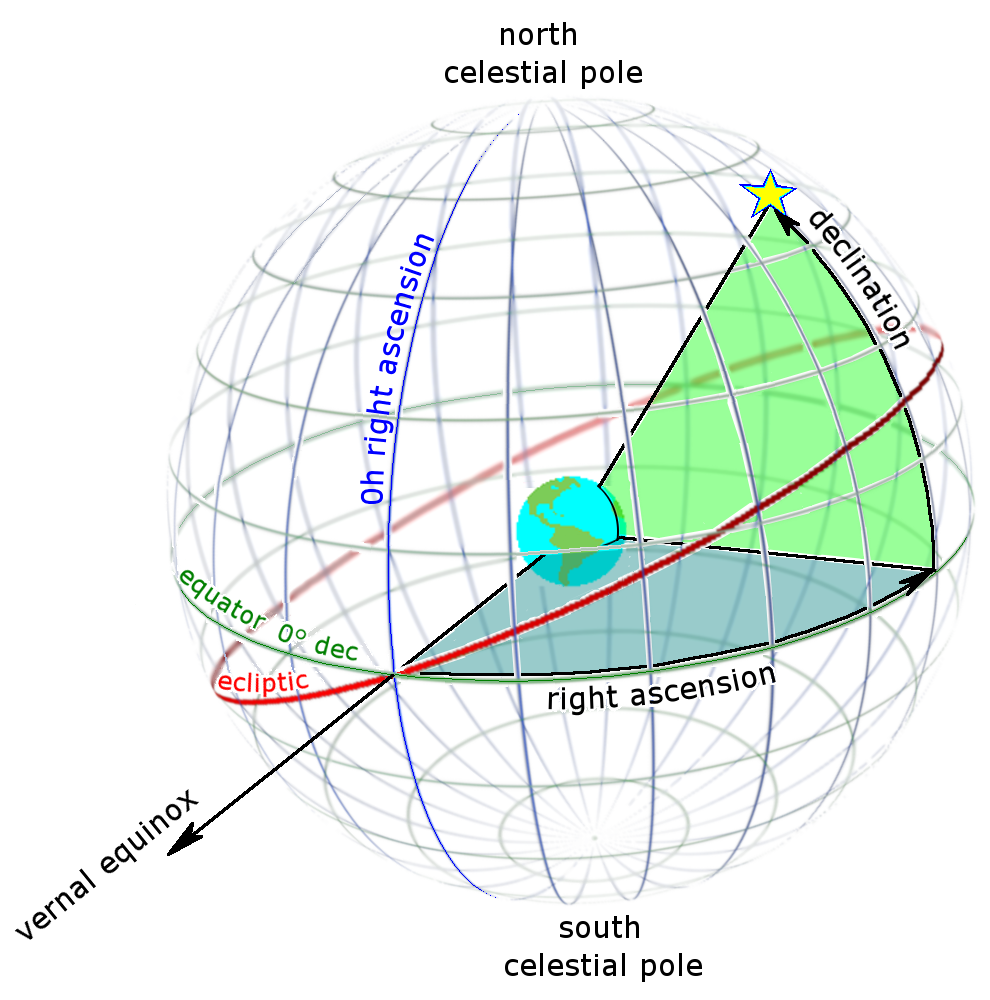
\includegraphics[scale=0.23]{Sun_global_coordinates_on_celestial_sphere.png}
    \caption{\small Visualization of global right ascension and declination \cite{WikipediaRightAscension}.}
    \label{fig:Sun_global_coordinates_on_celestial_sphere}
\end{figure}

Several factors affect the computation of the Sun's position, including the Earth's
axial tilt, which varies from 22 to 25 degrees over a period of approximately 41,000
years, and its orbital movement around the Sun, which alternates between a circular
and an elliptical orbit over a period of about 100,000 years. Additionally, the Earth
experiences a wobble, known as precession, in a cycle lasting around 23,000 years.
Gravitational interactions with the Moon and other planets, especially Jupiter and
Saturn, are primary contributors to these variations \cite[p.~2]{Muneer}. These and
other perturbations make accurate calculation of the Sun's position quite a difficult task.
The literature offers a wide variety of algorithms with different levels of accuracy
and complexity. Grena \cite{Grena} presents a set of five algorithms, valid from
2010 to 2100, that cover all possible applications in solar engineering. These
algorithms provide the Sun position angles \((\alpha_{\text{s}}, \psi_{\text{s}})\) in radians,
adhering to the conventions adopted in Section \ref{sec:Solar Geometry}. The
paper includes step-by-step descriptions optimized to reduce computational
complexity as much as possible. The calculations performed later
are based on the most accurate of these five algorithms, as the Sun's position
is required at sub-hourly intervals.

% \begin{table}[h]
%     \centering
%     \begin{tabular}{lcccc}
%         \toprule
%        \textbf{Panel type} & \textbf{Voc (V)} & \textbf{Isc (A)} & \textbf{Vmp (V)} \\
%         \midrule
%         Gruposolar GS601456P-218 & 36.30 & 8.19 & 29.00 & 7.55 \\
%         Kyocera KC175GHT-2 & 29.35 & 8.07 & 23.60 & 7.57 \\
%         Sanyo HIP-230 HDE1 & 42.46 & 7.26 & 34.00 & 6.87  \\
%         Shell S75 & 21.55 & 4.70 & 17.50 & 4.32 \\
%         \bottomrule
%     \end{tabular}
%     \caption{Data for the evaluation of the new model parameters.}
%     \label{table:model_parameters}
% \end{table}

% \begin{table}[h]
%     \centering
%     \begin{tabular}{lccccc}
%         \toprule
%         \textbf{Panel type} & \multicolumn{2}{c}{\textbf{Voc (V)}} & \textbf{Isc (A)} & \textbf{Vmp (V)} & \textbf{Imp (A)} \\
%         \cmidrule(r){2-3} % Draws a line under the Voc columns
%         & \textbf{Voc1} & \textbf{Voc2} & & & \\ % Voc1 and Voc2 are the new sub-column headers
%         \midrule
%         Gruposolar GS601456P-218 & 36.30 & (some value) & 8.19 & 29.00 & 7.55 \\
%         Kyocera KC175GHT-2 & 29.35 & (some value) & 8.07 & 23.60 & 7.57 \\
%         Sanyo HIP-230 HDE1 & 42.46 & (some value) & 7.26 & 34.00 & 6.87  \\
%         Shell S75 & 21.55 & (some value) & 4.70 & 17.50 & 4.32 \\
%         \bottomrule
%     \end{tabular}
%     \caption{Data for the evaluation of the new model parameters.}
%     \label{table:model_parameters_2}
% \end{table}

% \begin{table}[h]
%     \centering
%     \begin{tabular}{lccccc}
%         \toprule
%         \textbf{Panel type} & \multicolumn{2}{c}{\textbf{Voc (V)}} & \textbf{Isc (A)} & \textbf{Vmp (V)} & \textbf{Imp (A)} \\
%         \midrule
%         Gruposolar GS601456P-218 & 36.30 & (some value) & 8.19 & 29.00 & 7.55 \\
%         Kyocera KC175GHT-2 & 29.35 & (some value) & 8.07 & 23.60 & 7.57 \\
%         Sanyo HIP-230 HDE1 & 42.46 & (some value) & 7.26 & 34.00 & 6.87  \\
%         Shell S75 & 21.55 & (some value) & 4.70 & 17.50 & 4.32 \\
%         \bottomrule
%     \end{tabular}
%     \caption{Data for the evaluation of the new model parameters.}
%     \label{table:model_parameters_3}
% \end{table}

% \begin{table}[h]
%     \centering
%     \begin{tabular}{lccccc}
%         \toprule
%         \textbf{Panel type} & \multicolumn{2}{c}{\textbf{Voc (V)}} & \textbf{Isc (A)} & \textbf{Vmp (V)} & \textbf{Imp (A)} \\
%         \midrule
%         Gruposolar GS601456P-218 & 36.30 & (some value) & 8.19 & 29.00 & 7.55 \\
%         Kyocera KC175GHT-2 & 29.35 & (some value) & 8.07 & 23.60 & 7.57 \\
%         Sanyo HIP-230 HDE1 & 42.46 & (some value) & 7.26 & 34.00 & 6.87  \\
%         Shell S75 & 21.55 & (some value) & 4.70 & 17.50 & 4.32 \\
%         \bottomrule
%     \end{tabular}
%     \caption{Data for the evaluation of the new model parameters.}
%     \label{table:model_parameters_4}
% \end{table}

% \begin{itemize}
%     \item Global coordinates: solar declination and right ascension
%     \item Local coordinates: hour angle, solar altitude and azimuth 
% \end{itemize}

% The Greenwhich Hour Angle (GHA) is the angle measured westward of the
% Sun's position and the Greenwich meridian. In this context corresponds
% the Sun position to the longitude on which the point lies that is directly
% underneath the sun. This angle describes how far the sun moved westwards
% from the prime meridian. 

% Analogously to the GHA, the Local Hour Angle (LHA) measures how far the
% sun has moves westwards from the observers meridian. Hence it can be derived
% from the GHA and the observers longitude. 

% Solar time is a measure of time that depends on the position of the Sun in
% the sky. Solar noon occurs when the Sun is at its highest point in the sky,
% i.e. when the Sun crosses the local meridian. If it is 11 am solar time at
% a specific point on Earth, this means that the Sun is one hour away from solar
% noon for that location. Since the Earth rotates 15° of longitude per hour, the Sun is
% 15° to the east of the local meridian.

% The Equation of time (EOT) measured the time difference between solar time and
% the clock time.

% The solar day is the time between two successive solar noons and its length
% varies due to two main factors: the elliptical orbit of the earth and its
% axial tilt. As described by Kepler's law of planetary motion, the Earth's
% orbit around the Sun is not a perfect circle but an ellipse. This causes
% the Earth's speed in its orbit to vary: the Earth moves faster when it is
% closer to the Sun and slower when it is further away. This variation in
% speed causes the sun to appear more clickly (slowly) across the sky causing
% solar noon to arrive slightly earlier (later) each day.

% The declination angle is the angle between the equatorial plane and the line connecting
% the centres of the Sun and the Earth. It varies throughout the year due to the tilt
% of the Earth's axis relative to its orbit around the sun. The declination is positive
% in the Northern Hemisphere summer and negative in winter.

% The last global position angle, the Greenwhich Hour Angle, captures the position
% of the Sun in the sky. It ss the angle measured westward of the Sun's position
% and the Greenwich meridian. In this context corresponds the Sun position to
% the longitude on which the point lies that is directly underneath the sun.
% This angle describes how far the sun moved westwards from the prime meridian.

% The definition of the Greenwich Hour Angle also emphasized the need for
% convertions between the different time measurement systems, solar time and
% clock time, as the measurement of the Greenwich Hour Angle involves solar noon,
% the position when the sun is at its highest point. The difference between solar
% time and clocktime is given by the Equation of time.
\label{sec:Solar Geometry}
\subsection{Irradiance and radiation}
\label{sec:Irradiance and Radiation}
Solar radiation refers to the energy emitted by the Sun. The solar radiation received at Earth's
surface can be classified into two types: shortwave radiation with wavelengths between 0.29 and 4.0
\textmu m, and longwave radiation with wavelengths between 4 and 100 \textmu m. In the context of
photovoltaic energy generation, one is mainly concerned with shortwave radiation, as wavelengths
in the solar spectrum above 2.6 \textmu m contain very little energy.
Two terms frequently encountered in this context are irradiance and irradiation.
Irradiance, measured in \si{\watt\per\square\meter}, refers to the instantaneous flux of solar radiation
falling on any surface, while irradiation, measured in \si{\watt\hour\per\square\meter}, is the accumulated
energy flux incident on the surface over a given period of time. On its way to Earth's
surface, solar radiation interacts with atmospheric molecules. Therefore, the shortwave
solar radiation received on any surface can be divided into three components: 

\begin{itemize}
    \item \textbf{direct solar radiation \(B\)}: Solar radiation that reaches the surface without any interception
    \item \textbf{diffuse solar radiation \(D\)}: Solar radiation received after scattering and inter-reflection within the atmosphere.
    \item \textbf{reflected solar radiation \(R\)}: Solar radiation reflected from natural and human made surroundings.
\end{itemize}

\noindent
The sum of these components is termed global solar radiation (\(G\)) \cite[p. 2f]{CIBSE}.
Direct and global solar radiation are sometimes also referred to as beam and total
solar radiation, respectively. Figure \ref{fig:Radiation_components} visualizes the
three components of shortwave solar radiation.

\begin{figure}
    \centering
    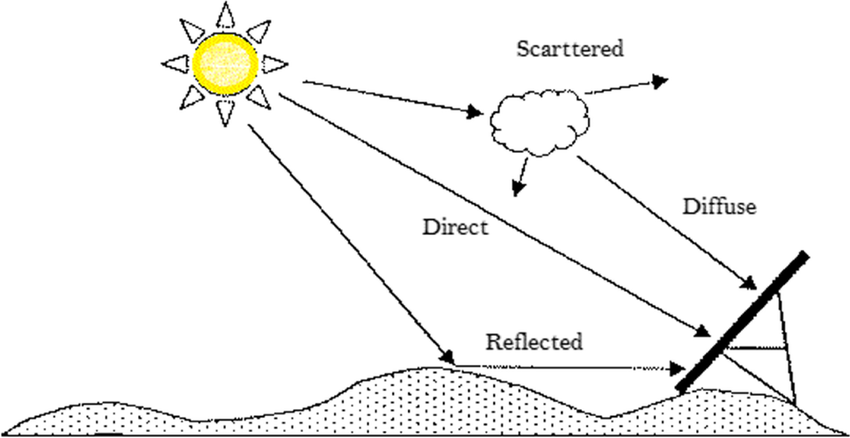
\includegraphics{Radiation_components.png}
    \caption{\small Visualization of shortwave radiation components \cite{Mghouchi}.}
    \label{fig:Radiation_components}
\end{figure}

The effect of clouds on solar radiation can be seen in Figure \ref{fig:DWD_irradiance_comparison},
which compares measured global radiation values received by a horizontally oriented surface on a
partially cloudy day with those measured on a sunny day. While the irradiance data on the sunny
day resemble a smooth haystack-shaped curve, the values on the cloudy day are much more volatile,
indicating the movement of clouds between the Sun and the measurement instrument. As clouds move
past the Sun, their edges can concentrate solar radiation and lead to short-lived spikes of up to 25 \%
increase. The spike in measured irradiance around 12:30 on the cloudy day is likely such an
occurrence \cite[p. 60]{Mayfield}.

\begin{figure}
    \centering
    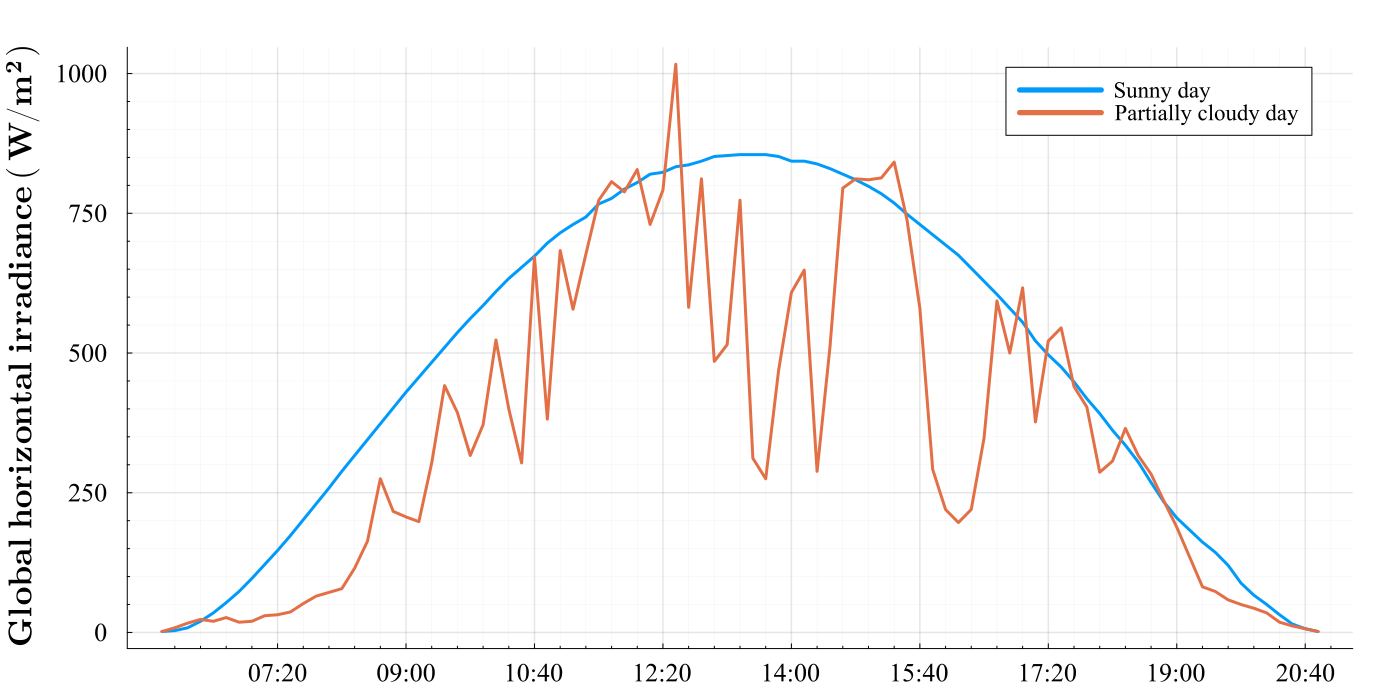
\includegraphics[scale=0.3]{DWD_irradiance_comparison.png}
    \caption{\small Global horizontal irradiance on a partially cloudy and sunny day \cite{DWD_weiherstephan_irradiance}.}
    \label{fig:DWD_irradiance_comparison}
\end{figure}

The strong influence of irradiance on photovoltaic energy generation is illustrated in Figure
\ref{fig:Surfclub_DC_output_comparison}. This figure compares the power output of a 4.62 kW
photovoltaic system on a cloudy and a sunny day, corresponding to the same days for which the
irradiance values were presented earlier. Although the photovoltaic system is not horizontally
oriented and is located approximately 18.4 km from the measurement instrument, a similar
pattern in the curves for each day is observed, indicating the well-known influence of solar
radiation on photovoltaic energy generation. It is worth mentioning that the time granularity
of the irradiance data is 10 minutes, slightly larger than the 5-minute granularity of the
photovoltaic system's production data. While the generation curve on the sunny day follows
a well-behaved approximate haystack-shaped curve, the curve on the cloudy day appears similarly
erratic. The early hours of the days provide valuable insights into irradiance values and power generation.
The PV system is shaded in the early hours due to its orientation and surrounding trees, decreasing
the amount of direct solar radiation. Interestingly, during these early hours, the measured horizontal
irradiance values on the sunny day exceed those on the cloudy day. Nevertheless, the power output in
the morning on the cloudy day is higher than on the sunny day, indicating overall more irradiance on
the PV modules due to increased diffuse radiation through clouds. This effect is confirmed by Figure
\ref{fig:DWD_diffuse_ratio}, which plots the diffuse ratio, the ratio between diffuse and global horizontal
radiation, for each of the analyzed days. The diffuse ratio on the sunny day illustrates the dominance
of direct radiation components, whereas the overcast day illustrates the contrary.

\begin{figure}
    \centering
    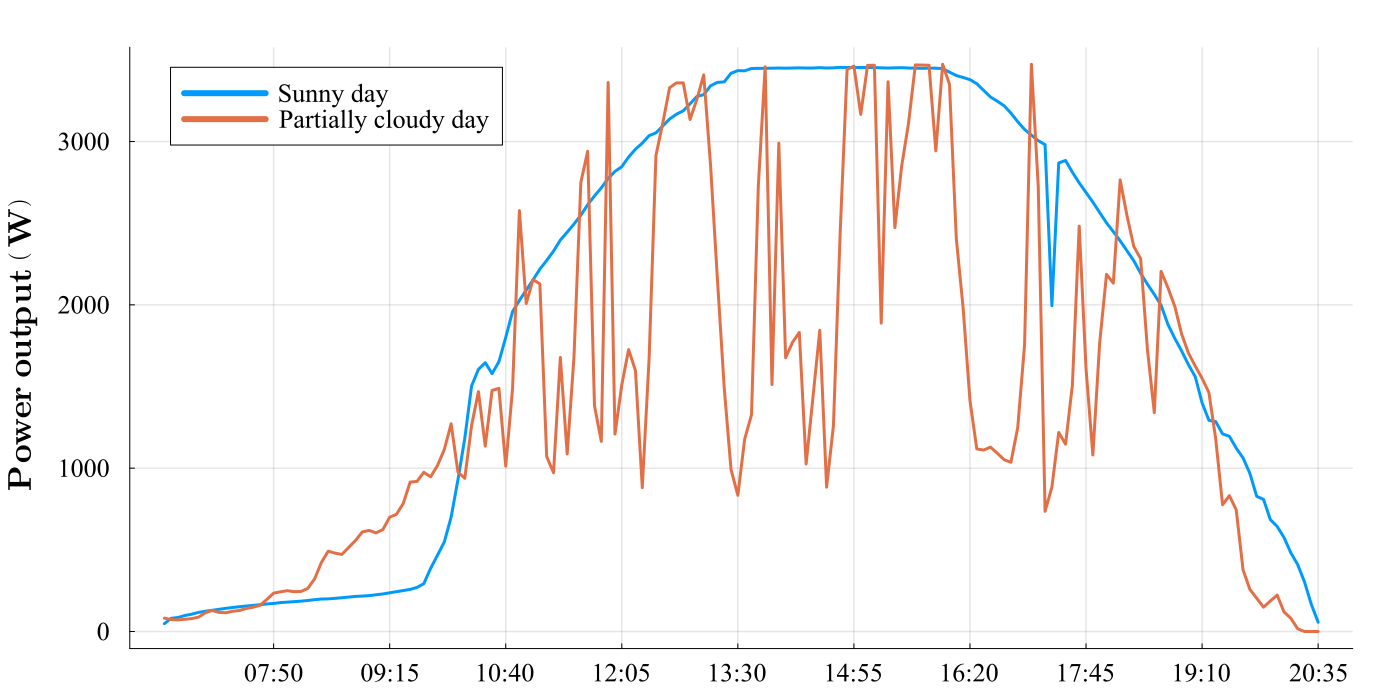
\includegraphics[scale=0.3]{Surfclub_DC_output_comparison.png}
    \caption{\small Power generation of a 4.62 kW photovoltaic system on a cloudy and sunny day.}
    \label{fig:Surfclub_DC_output_comparison}
\end{figure}

% NOTE: Kink in generation curve does not correspond to first timestamp where the solar elevation angle exceeds
% the surface tilt angle of 28°.

\begin{figure}
    \centering
    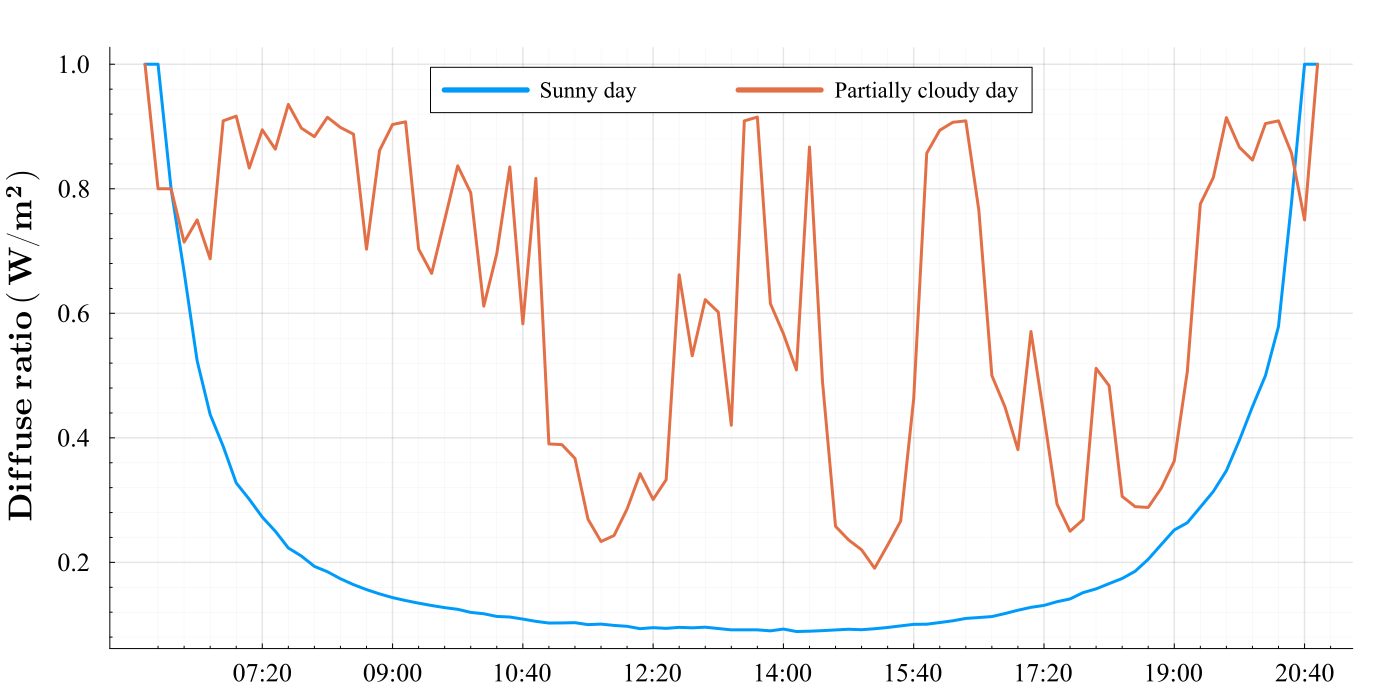
\includegraphics[scale=0.3]{DWD_diffuse_ratio.png}
    \caption{\small Comparision of diffuse ratio on a horizontal surface on a cloudy and sunny day \cite{DWD_weiherstephan_irradiance}.}
    \label{fig:DWD_diffuse_ratio}
\end{figure}
\subsection{Estimating in-plane irradiance}
\label{sec:Estimating in-plane irradiance}

Knowledge of the availability of solar irradiance for energy conversion in a region
or specific location is central to solar energy applications. PV collectors are often
installed on inclined surfaces, either constrained by the tilt of roofs or intentionally
angled to maximize annual electricity production or shift peak generation to a desirable
time of day. However, irradiance data are mostly measured or estimated for horizontal
surfaces, necessitating the conversion of horizontal irradiance to in-plane values.
Models performing this task are known as transposition models.
The irradiance components on a horizontal surface are termed global horizontal
irradiance \(G_{\text{h}}\), diffuse horizontal irradiance \(D_{\text{h}}\), and beam or direct
horizontal irradiance \(B_{\text{h}}\). Analogously, \(G_{\text{c}}\), \(D_{\text{c}}\),
and \(B_{\text{c}}\) refer to in-plane values, where the subscript \say{c} stands
for \say{collector}. Transposition models have the general form:

\begin{align}
    G_{\text{c}} &= B_{\text{c}} + D_{\text{c}} + R_{\text{c}}
    \label{eq:In_plane_irradiance_total} \\[8pt]
    B_{\text{c}} &= B_{\text{h}} \, \frac{\cos \nu}{\cos \psi_{\text{s}}}
    \label{eq:In_plane_irradiance_beam} \\[0pt]
    R_{\text{c}} &= G_{\text{h}} \, \tau_{R} \, \rho = G_{\text{h}} \, \frac{1 - \cos \beta}{2} \, \rho
    \label{eq:In_plane_irradiance_reflected} \\[8pt]
    D_{\text{\text{c}}} &= D_{\text{h}} \, \tau_{D}
    \label{eq:In_plane_irradiance_diffuse}
\end{align}

\noindent
Here, \(\nu\) is the solar incidence angle, \(\psi_{\text{s}}\) is the solar zenith angle,
\(\beta\) is the surface tilt angle as discussed in Section \ref{sec:Solar Geometry},
\(\rho\) is the albedo quantifying the ground's reflectivity, and \(\tau_{D}\) and \(\tau_{R}\)
are transposition factors for the diffuse and reflected components, respectively
\cite[p. 1f]{Quan2020}. As expected from the previous section, the global tilted
irradiance in Equation \ref{eq:In_plane_irradiance_total} is modeled as the sum
of the three irradiance components: beam, diffuse, and reflected.

The beam component in Equation \ref{eq:In_plane_irradiance_beam} follows a geometric
relation where the second factor adjusts the horizontal value \(B_{\text{h}}\). The latter can be
calculated as the difference between horizontal global irradiance \(G_{\text{h}}\) and diffuse
irradiance \(D_{\text{h}}\) \cite[p. 144]{Muneer}. To understand the formula, let \(B_{\text{n}}\) denote
the direct normal irradiance received by a surface perpendicular to the sun's rays.
The in-plane beam irradiance B received by any surface with incidence angle \(\nu\), 
assuming parallel sun rays, is expressed as:

\begin{equation}
    B = B_{\text{n}} \cos \nu
    \label{eq:In_plane_beam_irradiance_derivation}
\end{equation}

\noindent
This equation implies that a surface tilted away from the sun's rays by angle \(\nu\)
receives only a fraction of the direct normal radiation \(B_{\text{n}}\), given by \(\cos \nu\).
This fraction equals the proportion of the surface's projection onto a plane perpendicular
to the sun rays. Figure \ref{fig:In_plane_beam_irradiance_derivation_visualization}
illustrates this derivation. Application of Equation \ref{eq:In_plane_beam_irradiance_derivation}
to a horizontal and a tilted surface, denoted by subscripts \say{h} and \say{c} respectively,
yields:

\begin{align}
    B_{\text{h}} &= B_{\text{n}} \cos \psi_{\text{s}} \\[7pt]
    B_{\text{c}} &= B_{\text{n}} \cos \nu \\[4pt]
    \Rightarrow B_{\text{c}} &= B_{\text{h}} \, \frac{\cos \nu}{\cos \psi_{\text{s}}}
\end{align}

\noindent
where in the case of a horizontal surface, \(\nu = \psi_{\text{s}}\).

As mentioned in \cite{SandiaNationalLaboratory}, the ground-reflected irradiance on a tilted
surface \(R_{\text{c}}\) is calculated based on the irradiance on the ground, the ground's reflectivity
\(\rho\), and the surface tilt angle \(\beta\). Equation \ref{eq:In_plane_irradiance_reflected} assumes,
among other things, that the ground irradiance is uniform, equal to \(G_{\text{h}}\) and reflected equally
in all directions, that is, the ground acts as a Lambertian reflector. These idealized assumptions,
resulting in the common transposition factor \(\tau_{R} = \frac{1 - \cos \beta}{2}\), are widely used
in transposition calculations despite their limitations \cite{Gueymard2017, Quan2020}. Table
\ref{tab:Reflected_in_plane_irradiance_transposition_factor_for_different_surface_tilts}
summarizes how the ground transposition factor and the reflected component change with different surface tilts.
As the tilt angle increases, the surface starts to \say{see} more of the ground and receives therefore more
ground-reflected irradiance. The transposition factor smoothly transitions between 0 and \(\frac{1}{2}\)
as \(\beta\) varies from \(0^\circ\) to \(90^\circ\). Equation \ref{eq:In_plane_irradiance_reflected}
uses a constant albedo value. Figure \ref{fig:Albedo_variability} illustrates the variability of
measured reflectivity at a station in Murcia, Spain, during representative days in winter and summer, as well as throughout the year.
Clearly, assuming a constant albedo is idealistic and can increase the transposition model's error.
Unfortunately, accurate information on a site's surroundings is rarely available. The PVsyst
modeling software provides guidance for estimating albedo values, as presented in Table
\ref{tab:Sandia_National_Laboratories_albedo}.

\begin{table}
    \centering
    \begin{tabular}{ll}
        \toprule
        \textbf{Surface} & \textbf{Albedo \(\rho\)} \\
        \midrule
        Urban environment & 0.14-0.22 \\
        Grass & 0.15-0.25 \\
        Fresh grass & 0.26 \\
        Fresh snow & 0.82 \\
        Wet snow & 0.55-0.75 \\
        Dry asphalt & 0.09-0.15 \\
        Wet asphalt & 0.18 \\
        Concrete & 0.25-0.35 \\
        Red tiles & 0.33 \\
        Aluminum & 0.85 \\
        Copper & 0.74 \\
        New galvanized steel & 0.35 \\
        Very dirty galvanized steel & 0.08 \\
        \bottomrule
    \end{tabular}
    \caption{\small Estimates of ground albedo values for various surfaces \cite{SandiaNationalLaboratory}.}
    \label{tab:Sandia_National_Laboratories_albedo}
\end{table}

\begin{figure}
    \centering
    \subfloat[\centering]{{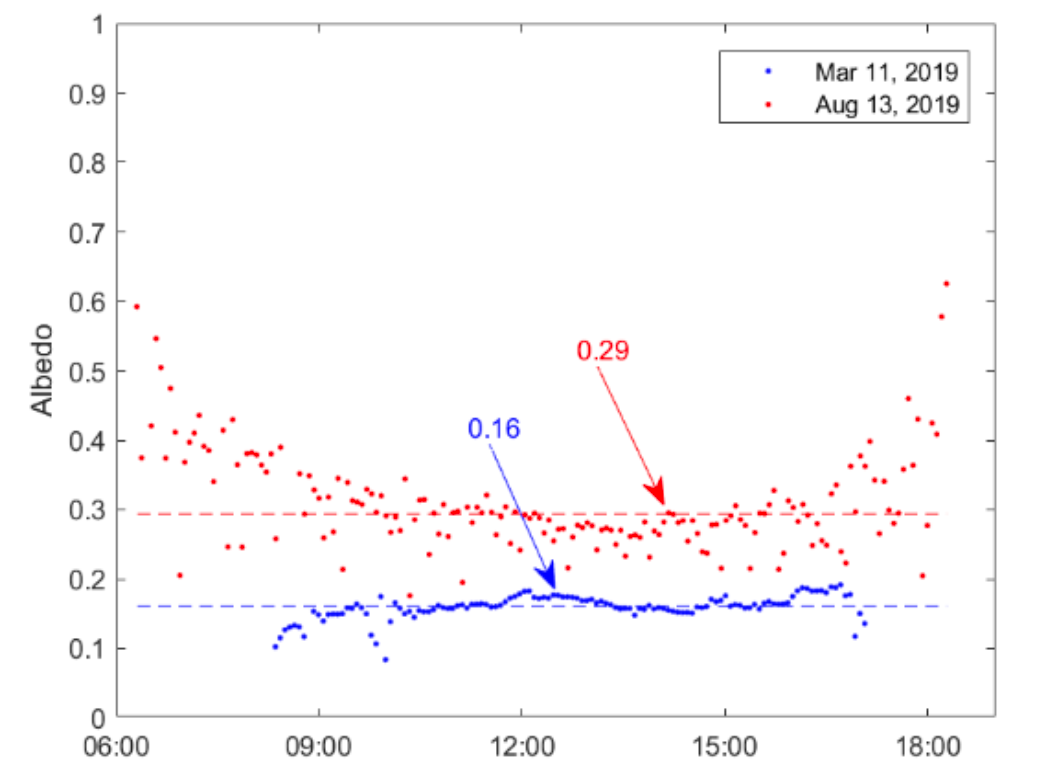
\includegraphics[width=7.1cm]{Albedo_variability_throughout_the_year.png} }}
    \qquad
    \subfloat[\centering]{{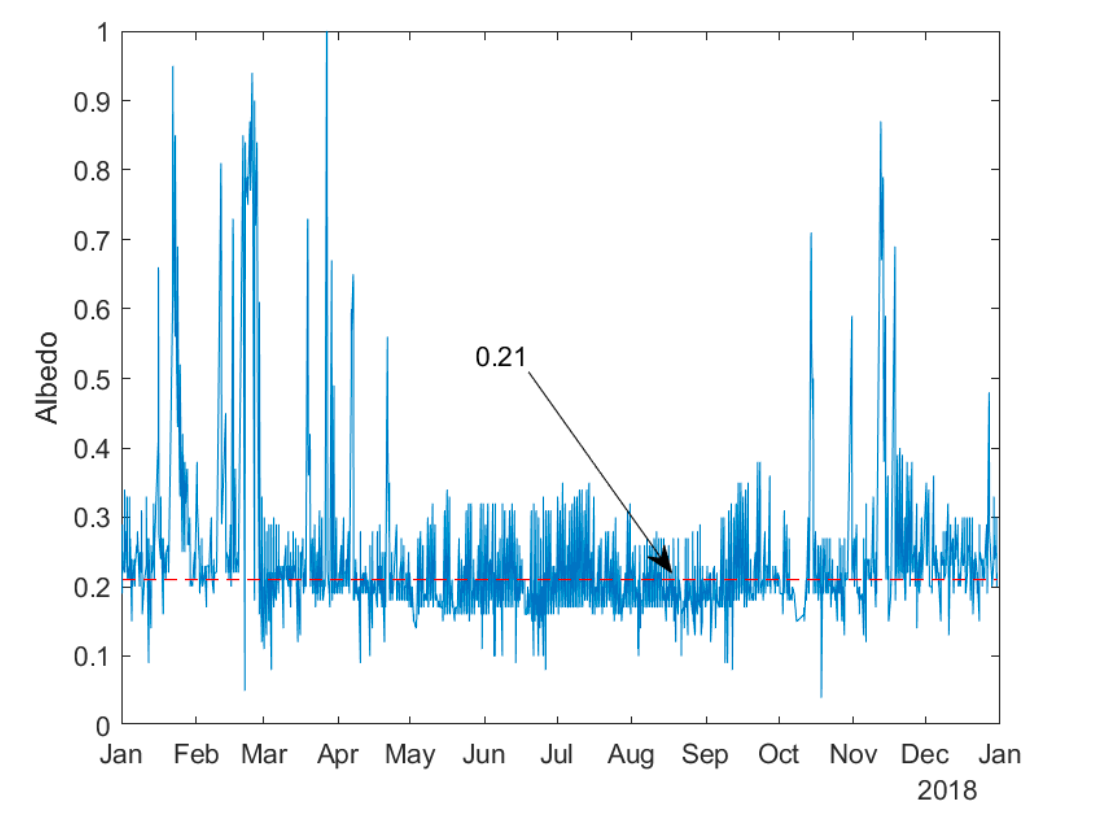
\includegraphics[width=7cm]{Albedo_variability_on_two_days.png} }}
    \caption{\small Variability of albedo during the day a) and throughout the year b) with indication
        of median values \cite{Toledo}.}
    \label{fig:Albedo_variability}
\end{figure}

\begin{table}
    \centering
    \renewcommand{\arraystretch}{1.25}
    \begin{tabular}{lll}
        \toprule
        \textbf{Surface tilt} \(\beta\) & \textbf{Transposition factor} \(\tau_{R} \)& \textbf{Reflected component} \(R_{\text{c}}\) \\
        \midrule
        \(0^\circ\) & 0 & 0  \\
        \(90^\circ\) & \(\frac{1}{2}\) & \(G_{h} \rho \frac{1}{2}\) \\
        \(\beta \in (0^\circ, 90^\circ)\) & \(\frac{1 - \cos \beta}{2} \in (0, \frac{1}{2})\) & \(G_{h} \: \rho \: \frac{1 - \cos \beta}{2}\) \\
        \bottomrule
    \end{tabular}
    \caption{\small Equation \ref{eq:In_plane_irradiance_reflected} for different surface tilts.}
    \label{tab:Reflected_in_plane_irradiance_transposition_factor_for_different_surface_tilts}
\end{table}

\begin{figure}
    \centering
    \begin{tabular}{@{}cc@{}}
        \begin{tikzpicture}
            \coordinate (center) at (3,0);
            \coordinate (left) at (0,0);
            \coordinate (right) at (6,0);
            \coordinate (top) at (3,3);
            \coordinate (A) at (0.401923788646684,1.4999999999999998);
            \coordinate (A_inside) at (1.2679491924311226, 0.9999999999999999);
            \coordinate (B) at (1.5000000000000007,2.598076211353316);
            \coordinate (B_inside) at (2.5, 0.8660254037844387);
            \coordinate (C) at (3.0179491924311224, 4.031088913245535);
            \coordinate (D) at (5.531088913245536, 2.6160254037844384);

            \draw (0,0) -- (6,0) node[above, near end, black, xshift = -0.5pt] {\tiny horizontal plane};
            \draw[thick] (center) -- (A) node[pos = 1, above, black] {\tiny surface};
            \draw (A_inside) -- (C) node[at end, black, above] {\tiny normal to surface};
            \draw[dashed, thick, black] (center) -- (B);
            \draw[dashed, black] (B_inside) -- (D) node[at end, above, black] {\tiny shifted normal};

            \pic [draw, <-, angle radius=1.5cm, "$\nu$", black] {angle = B--center--A};
        \end{tikzpicture} & 
        \begin{tikzpicture}
            \coordinate (center) at (3,0);
            \coordinate (left) at (0,0);
            \coordinate (right) at (6,0);
            \coordinate (top) at (3,3);

            \coordinate (A) at (0.401923788646684,1.4999999999999998);
            \coordinate (A_inside) at (1.2679491924311226, 0.9999999999999999);
            \coordinate (B) at (1.5000000000000007,2.598076211353316);
            \coordinate (B_inside) at (2.5, 0.8660254037844387);
            \coordinate (C) at (3.7679491924311224,5.330127018922193);
            \coordinate (D) at (6.830127018922194, 3.3660254037844384);

            \coordinate (E) at (3.866025403784439, 3.4999999999999996);
            \coordinate (F) at (6.464101615137755, 1.9999999999999998);
            \coordinate (G) at (1.7009618943233424, 2.2500000000000004);

            \draw (0,0) -- (6,0);
            \draw (0,0) arc[start angle=180, end angle=0, radius=3cm];
            \draw[thick] (center) -- (A);
            \draw[dashed, black] (center) -- (B);        
            \draw[dashed, thick, black] (A) -- (E) node[pos=1, yshift = -3pt, above, black] {\tiny Sun rays || shifted normal};
            \draw[dashed, thick, black] (center) -- (F) node[midway, above, sloped, black] {\tiny Sun ray};
            \draw[thick] [decorate, decoration = {calligraphic brace, amplitude = 7pt, mirror}] (center) -- (G) node[midway, above, sloped, black, yshift = 5pt] {\tiny $\cos \nu$};
            
            \pic [draw, <-, angle radius=1.5cm, "$\nu$", black] {angle = B--center--A};
        \end{tikzpicture} \\ (a) \: \: & (b) \: \:
    \end{tabular}
    \caption{\small Visualization of the relation between the beam irradiance received
        by a perpendicular surface and a surface with incidence angle \(\nu\).}
    \label{fig:In_plane_beam_irradiance_derivation_visualization}
\end{figure}

The interaction of solar radiation with the atmosphere results in the diffuse component 
\(D_{\text{c}}\) mentioned in Section \ref{sec:Irradiance and Radiation}. On one hand, it is subject
to attenuation and absorption by atmospheric molecules such as water vapor (H$_2$O), ozone
(O$_3$), and carbon dioxide (CO$_2$). On the other hand, it is scattered by molecules like
nitrogen (N$_2$) and oxygen (O$_2$) distributed throughout the sky dome. Figure
\ref{fig:Absorption_of_solar_radiation} shows the absorption of shortwave radiation
due to various atmospheric constituents, indicated by dips in the curves.
From a modeling perspective, two types of transposition models exist:
isotropic and anisotropic. These models assume a uniform versus non-uniform
distribution of the diffuse component over the sky, respectively \cite[p. 5]{Toledo}.
The interactions between atmospheric molecules and radiation suggest that an isotropic
model may be too inaccurate for the diffuse component, a notion confirmed by several
comparison studies \cite{Hay1985, PerezDriesse2024}. Numerous transposition models
are documented in the literature, along with abundant evaluation studies. The
comprehensive study by Yang et al. \cite{Yang2016} analyzed the accuracy of 26
transposition models using one year of solar irradiance measurements from four
locations. Although no universal model outperformed all others in every case study,
some were recommended. These include the family of Perez models, particularly a
representative version described in the remainder of this section.

The first version of the anisotropic Perez model \cite{Perez1986} divided the sky hemisphere
into three zones to account for the main anisotropy observed in the atmosphere: circumsolar
brightening due to forward scattering by aerosols and horizon brightening primarily due to
multiple Rayleigh scattering and backscattering in clear atmospheres. Figure \ref{fig:Perez_sky_dome}
shows the geometrical representation of these three zones. The circumsolar region is a
reversed cone with a radius \(\alpha = 15^\circ\), centered on the Sun's position, and the
horizon band is defined by an angular thickness \(\zeta = 6.5^\circ\).
The authors derived the model's governing equation from two expressions that describe how
the horizontal diffuse irradiance and the irradiance received by a tilted surface can be
calculated under the assumption that the radiances originating from the main portion of
the dome, the circumsolar region, and the horizon zone are respectively equal to \(L\), \(F_{1} L\),
and \(F_{2} L\). The products are indicated as \(F_{i} \times L\) in the illustration. The
non-dimensional coefficients \(F_{1}\) and \(F_{2}\) were the only undefined terms in
the model's equation. Least-squares fitting of measured data on sloped surfaces from
four sites with different climatic conditions was performed to obtain values for these
coefficients across 240 sky condition categories \cite[p. 481ff]{Perez1986}.
The next publication on the model \cite{Perez1987} aimed to simplify the model while maintaining or improving
its accuracy. A major simplification was rewriting the governing equation in terms of reduced
brightness coefficients, allowing for negative values to cover a broader range of sky conditions.
Additional simplifications included treating the horizon band as an infinitesimally thin region
at 0° elevation and considering the circumsolar energy as originating from a point source.
\cite[p. 222ff]{Perez1987}. Building upon these simplifications, the point source version of the model, as presented
in \cite{Perez1990}, is based on the previous considerations and is the version employed in this thesis.
This model estimates the incident diffuse energy on any tilted surface using the following equation:

\begin{figure}
    \centering
    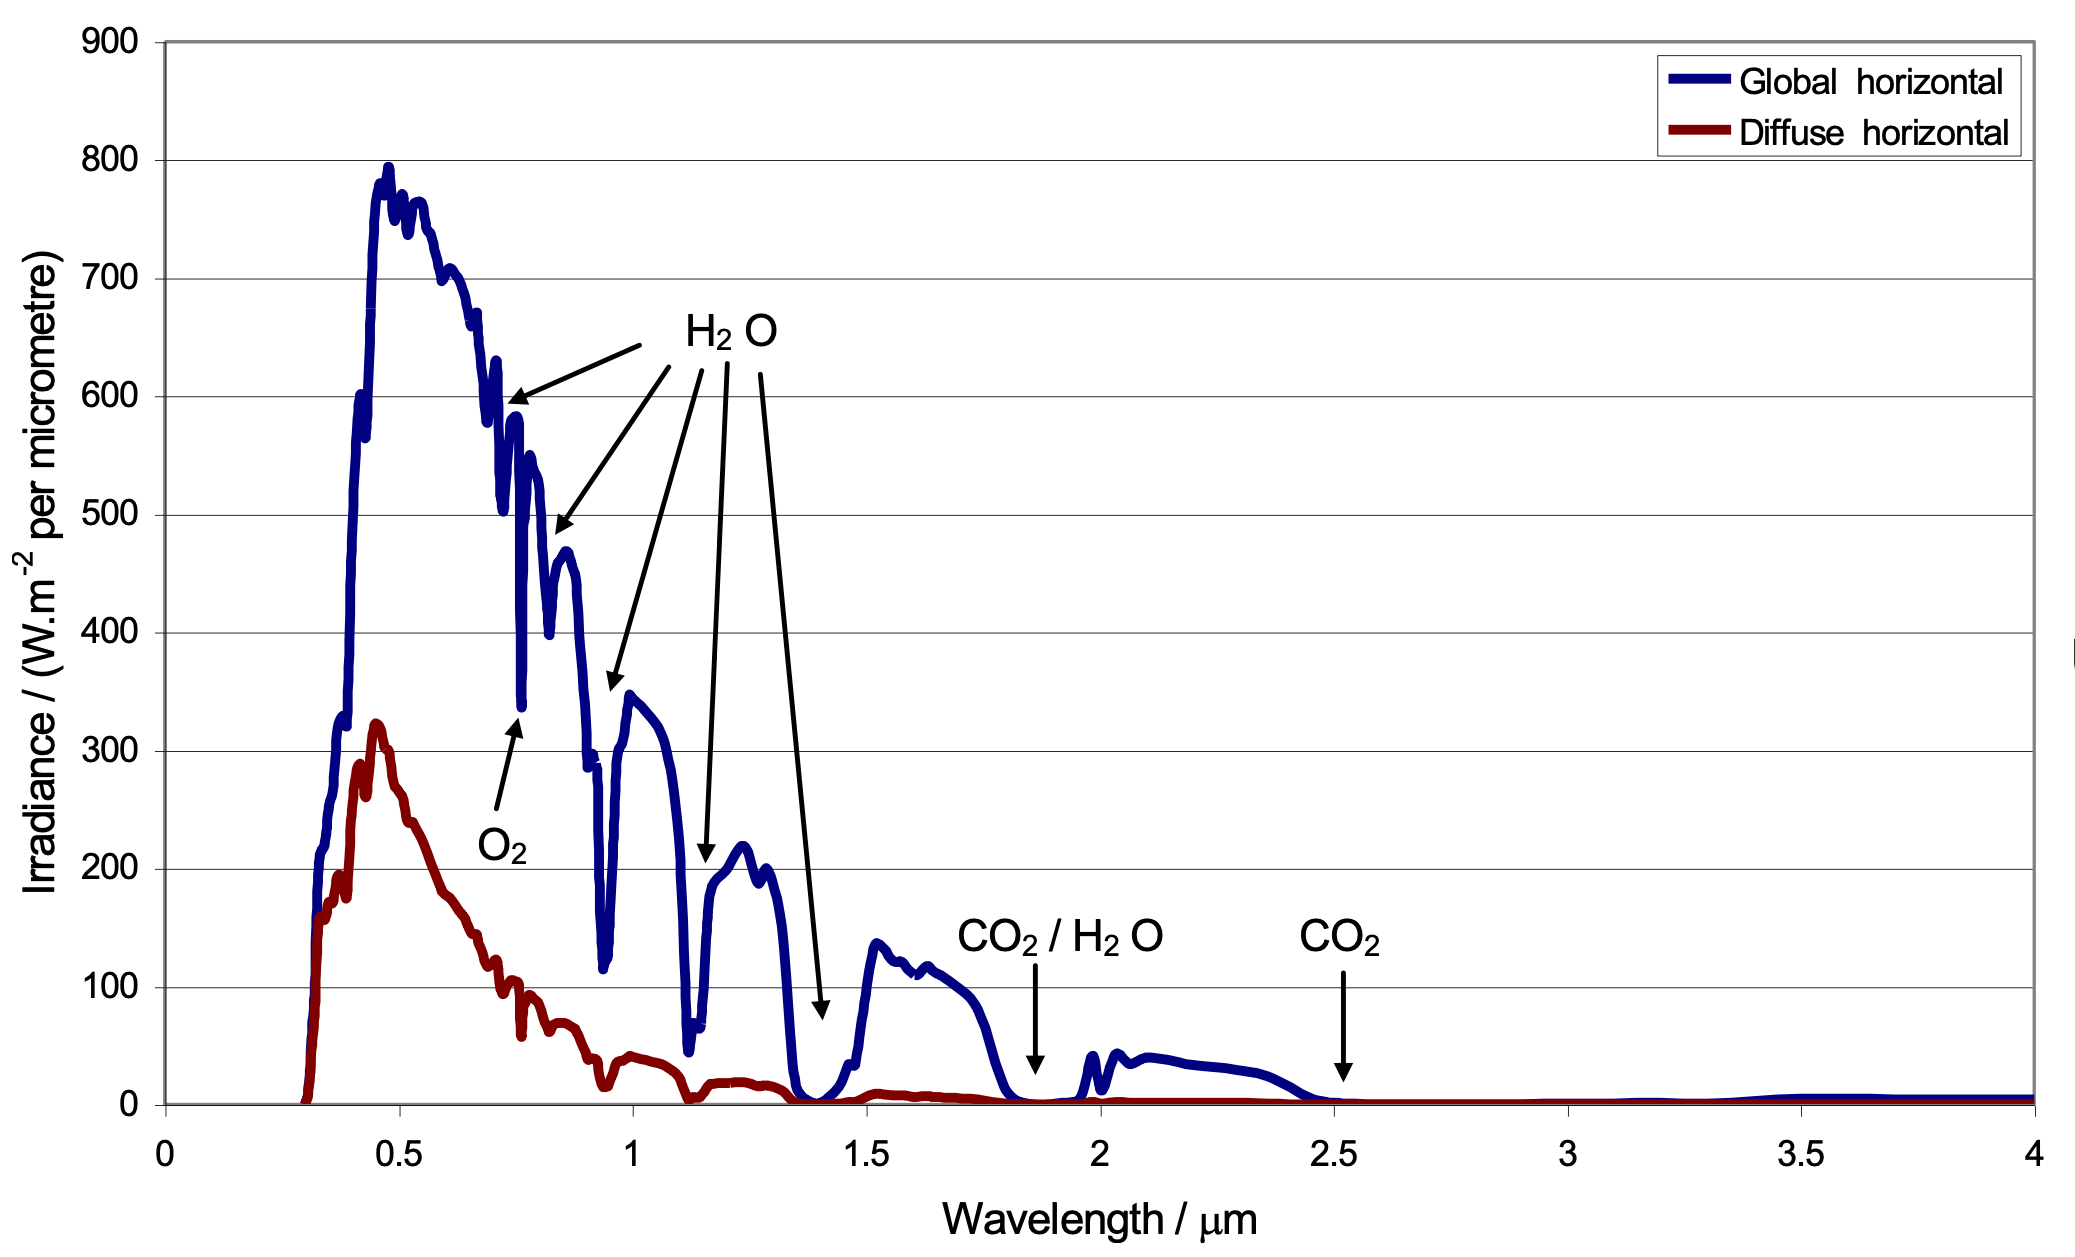
\includegraphics[scale=0.17]{Solar_Geometry_absorption_of_solar_radiation.png}
    \caption{\small Absorption of radiation due to various atmospheric constituents \cite{CIBSE}.}
    \label{fig:Absorption_of_solar_radiation}
\end{figure}

\begin{figure}
    \centering
    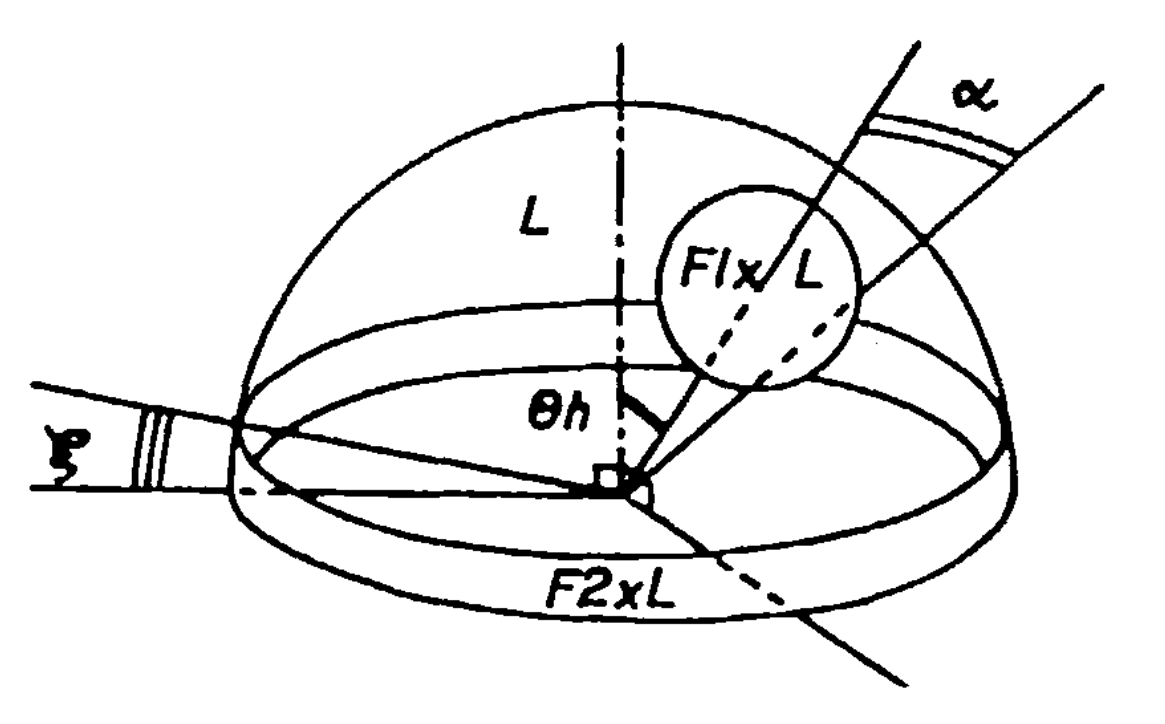
\includegraphics[scale=0.23]{Perez_sky_dome.png}
    \caption{\small Geometrical representation of the sky dome in Perez's slope irradiance model \cite{Perez1986}.}
    \label{fig:Perez_sky_dome}
\end{figure}

% \begin{table}[H]
%     \centering
%     \begin{tabular}{l|c|c|c|l}
%         \toprule
%         Station & Latitude & Longitude & Elevation & Climate Type \\
%         \midrule        
%         Albany, New York & 42° 42'N & 73° 50'W & 94m & Humid \\
%         &          &           &     & Continental \\
%         &          &           &     & Temperate \\
%         San Antonio, Texas & 29° 46'N & 98° 49'W & 253m & Semi-arid \\
%                 &          &           &      & Sub tropical \\
%         Carpentras, France & 44° 05'N & 5° 03'E & 99m & Mediterranean \\
%         Trappes, France & 48° 46'N & 2° 0'E & 167m & Marine \\
%             &          &         &      & Temperate \\
%         \bottomrule
%     \end{tabular}
%     \caption{Description of selected sites \cite{Perez1986}.}
%     \label{tab:Perez1986_sites}
% \end{table}

\begin{equation}
    D_{\text{c}} = D_{\text{h}} \: \biggl[ (1-F_{1}) \: \frac{1 + \cos \beta}{2} + F_{1}\frac{a}{b} + F_{2} \sin\beta\biggr]
    \label{eq:Perez_in_plane_irradiance}
\end{equation}

\noindent
Here, the second factor on the right side is the diffuse transposition factor \(\tau_{D}\)
from Equation \ref{eq:In_plane_irradiance_diffuse}. The terms \(a\) and \(b\) account for the 
angles of incidence of circumsolar radiation on the tilted and horizontal surfaces, 
respectively:

\begin{align}
    a &= \max\{0, \cos\nu\} \\
    b &= \max\{\cos85^\circ, \cos \psi_{\text{s}}\}
\end{align}

\noindent
The anisotropic coefficients \(F_{1}\) and \(F_{2}\) express the degree of circumsolar and horizon anisotropy,
respectively. They are functions of the sky conditions, characterized by the solar zenith angle
\(\psi_{\text{s}}\), the clearness index \(\epsilon\), and the brightness index \(\Delta\):

\begin{align}
    F_{1} &= \min \Bigl\{ 0.9, \max\bigl\{0, f_{11}(\epsilon) + f_{12}(\epsilon)\Delta + \frac{\pi \psi_{\text{s}}}{180}f_{13}(\epsilon) \bigr\} \Bigr\}
    \label{eq:brightness_coefficient_circumsolar} \\
    F_{2} &= f_{21}(\epsilon) + f_{22}(\epsilon)\Delta + \frac{\pi \psi_{s}}{180}f_{23}(\epsilon)
    \label{eq:brightness_coefficient_horizon}
\end{align}

\noindent
Following recommendations from \cite{PerezDriesse2024}, a limit of 0.9 is imposed on \(F_{1}\) to
ensure physically coherent results. The clearness index \(\epsilon\) is calculated as:

\begin{equation}
    \epsilon = \frac{\bigl(\frac{D_{\text{h}} + B_{\text{n}}}{D_{\text{h}}}\bigl) + 5.535\cdot10^{-6} \psi_{\text{s}}^3}{1 + 5.535\cdot10^{-6} \psi_{\text{s}}^{3}}
\end{equation}

\noindent
The brightness index \(\Delta\) is given by:

\begin{equation}
    \Delta = m_{\text{air}} \, \frac{D_{\text{h}}}{G_{\text{e}}}
\end{equation}

\noindent
where \(m_{\text{air}}\) is the air mass and \(G_{\text{e}}\) is the extraterrestrial normal irradiance.
As referenced in \cite{Toledo}, the air mass can be calculated using the empirical
equation by Kasten and Young \cite{Karsten}:

\begin{equation}
    m_{\text{air}} = \frac{\exp(-0.0001184h)}{\cos(\psi_{\text{s}}) + 0.5057(96.080 - \psi_{\text{s}})^{-1.634}}
\end{equation}

\noindent
Here, \(h\) is the site altitude in meters. The extraterrestrial irradiance is calculated using 
Spencer's formula \cite{Spencer1971Fourier}, with an accuracy of \(\pm0.01\%\):

\begin{align}
    G_{\text{e}} = 1367 \: \bigl(&1.00011 + 0.034221 \cos Q + 0.00128 \sin Q \nonumber \\ 
                     &+ 0.000719 \cos 2Q + 0.000077 \sin2Q\bigr)
\end{align}

\noindent
where 1367 is the solar constant (\si{\watt\per\square\meter}) and \(Q\) is given by:

\begin{equation}
    Q = (n_{\text{day}} - 1) \frac{360}{365}
\end{equation}

\noindent
with \(n_{\text{day}}\) being the nth day of the year. A recommended set of coefficients for
calculating the brightness coefficients in Equations \ref{eq:brightness_coefficient_circumsolar}
and \ref{eq:brightness_coefficient_horizon} is provided in Table
\ref{tab:Perez_coeff}. These coefficients were fitted using data
from 10 American and three European cities covering different climatic
environments. Table \ref{tab:Perez_experimental_data} summarizes the
climatic environments and datasets used.
The discrete sky clearness categories range from overcast in the first
row to clear in the last row \cite[p. 273]{Perez1990}. These coefficients
could be fitted to a local climate if high-quality datasets of measured
sloped irradiance for different orientations, along with corresponding
meteorological data, are available. 

\begin{table}
    \resizebox{\columnwidth}{!}{
        \begin{tabular}{c S S S S S S}
            \toprule
            Sky clearness \(\epsilon\) & {$f_{11}$} & {$f_{12}$} & {$f_{13}$} & {$f_{21}$} & {$f_{22}$} & {$f_{23}$} \\
            \midrule
            $[1.000, 1.065)$ & -0.0083 & 0.5877 & -0.0621 & -0.0596 & 0.0721 & -0.0220 \\
            $[1.065, 1.230)$ & 0.1299  & 0.6826 & -0.1514 & -0.0189 & 0.0660  & -0.0289 \\
            $[1.230, 1.500)$ & 0.3297  & 0.4869 & -0.2211 & 0.0554  & -0.0640 & -0.0261 \\
            $[1.500, 1.950)$ & 0.5682  & 0.1875 & -0.2951 & 0.1089  & -0.1519 & -0.0140 \\
            $[1.950, 2.800)$ & 0.8730   & -0.3920 & -0.3616 & 0.2256  & -0.4620  & 0.0012 \\
            $[2.800, 4.500)$ & 1.1326  & -1.2367 & -0.4118 & 0.2878 & -0.8230  & 0.0559 \\
            $[4.500, 6.200)$ & 1.0602  & -1.5999 & -0.3589 & 0.2642 & -1.1272 & 0.1311 \\
            $[6.200, \infty)$ & 0.6777  & -0.3273 & -0.2504 & 0.1561 & -1.3765 & 0.2506 \\
            \bottomrule
        \end{tabular}
    }
    \caption{\small Coefficients for Perez slope irradiance model \cite[Ch.\ 4]{Muneer}.}
    \label{tab:Perez_coeff}
\end{table}

\begin{table}[H]
    \centering
    \resizebox{\columnwidth}{!}{
        \begin{tabular}{lll}
            \toprule
            \textbf{Site} & \textbf{Main Environmental Fatures} & \textbf{Span and Frequency} \\
            \midrule
            Geneva, & Temperate maritime, with central Europe & 1 yr. hourly data \\
            Switzerland & continental influence. Persistent &  \\
            & nebulosity enhanced by blocking position &  \\
            & at foot-hill of the Alps. &  \\
            % \midrule
            % & & \\
            Trappes, & Temperate maritime with high incidence of & 3 yr. hourly data \\
            France & intermediate skies. &  \\
            % \midrule
            % & & \\
            Carpentras, & Mediterranean & 3 yr. hourly data \\
            France & & \\
            % \midrule
            % & & \\
            Albany, & Humid continental with bimodal influence & 3 yr. hourly data \\
            NY, USA & & 2 yr. 15 min. data \\
            % \midrule
            % & & \\
            New York, & Humid continental with maritime influence & 1 yr. 15 min. data \\
            NY, USA & plus large city's anthropogenic environment &  \\
            % \midrule
            % & & \\
            Farmingdale, & Same as above but without city's environment & 1 yr. 15 min. data \\
            NY, USA & & \\
            % \midrule
            % & & \\
            Oswego, & Humid continental, Great Lakes basin & 6 mo. 15 min. data \\
            NY, USA & & \\
            % \midrule
            % & & \\
            Glens Falls, & Humid continental & 6 mo. 15 min. data \\
            NY, USA & & \\
            % \midrule
            % & & \\
            Phoenix, & Arid, low elevation & 6 mo. hourly data \\
            AZ, USA & & \\
            % \midrule
            % & & \\
            Albuquerque, & Arid, high elevation (1800 m) & 1 yr. hourly data \\
            NM, USA & & \\
            % \midrule
            % & & \\
            Los Angeles, & Arid and maritime influence plus high & 6 mo. hourly data \\
            CA, USA & frequency of anthropogenic smog events &  \\
            % \midrule
            % & & \\
            Osage, & Continental, U.S. Great Plains & 6 mo. hourly data \\
            KS, USA & & \\
            % \midrule
            % & & \\
            C. Canaveral, & Subtropical, low latitude, maritime & 6 mo. hourly data \\
            FL, USA & & \\
            \bottomrule
        \end{tabular}
    }
    \caption{\small Origin, size, and climatic environment of experimental data sets \cite{Perez1990}.}
    \label{tab:Perez_experimental_data}
\end{table}

% \begin{figure}
%     \centering
%     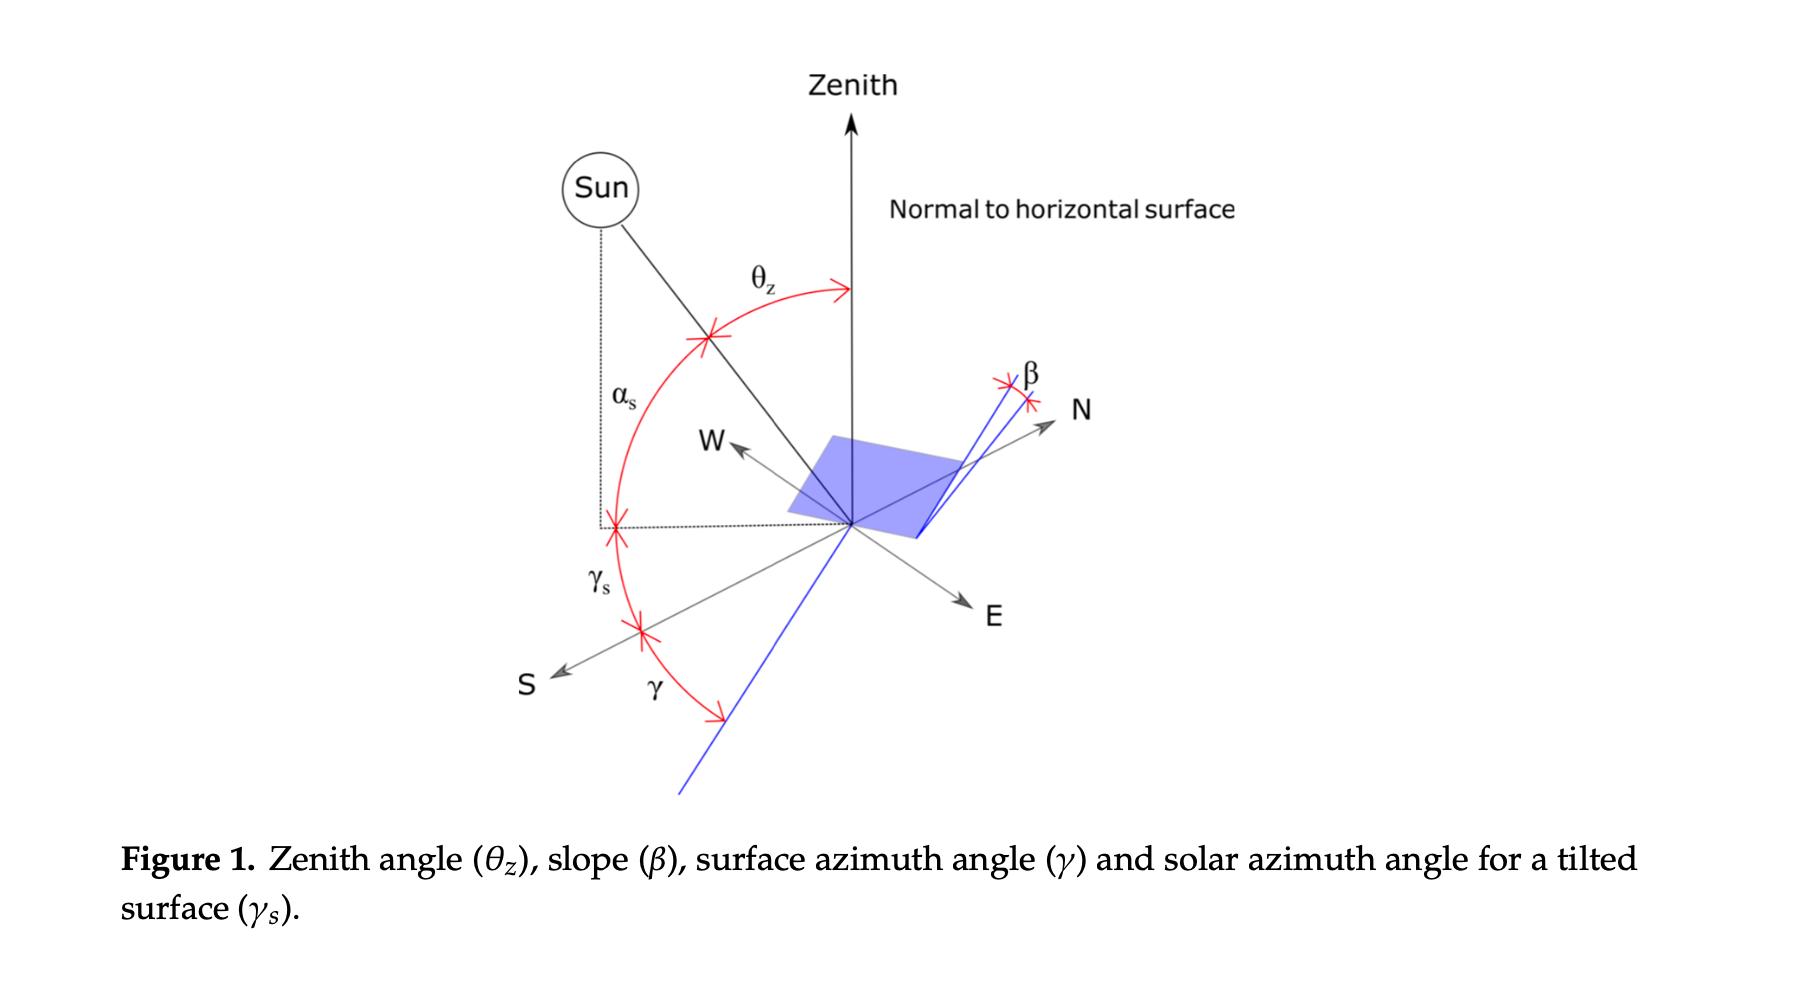
\includegraphics[scale=0.23]{Solar_Geometry_Toledo.png}
%     \caption{Solar geometry here just as a reference during thesis developement \cite{CIBSE}.}
% \end{figure}
\newpage

\section{Photovoltaic system modeling and power prediction}
\label{sec:Photovoltaic system modeling and power prediction}
This chapter introduces the physical model used in this thesis.
This so-called five-parameter model is one of several physical
models discussed in the literature. The chapter begins with a
brief review of these models. Understanding their application 
involves two key concepts covered in distinct sections:
operating conditions and current-voltage characteristics.
The operating conditions are the input parameters for the
physical models. In real-world scenarios, these often need
to be estimated from meteorological data, as is the case in
this thesis. The current-voltage (I-V) characteristic is a
graphical representation of the relationship between the
current and voltage of an electrical device. The physical
models aim to characterize the I-V characteristics
of the PV device under study. The chapter concludes with a
description of how the presented physical model can be
applied to simulate arbitrary configurations of PV systems,
given certain assumptions.

\subsection{Background to physical models}
As illustrated in Figure \ref{fig:PV_system_configuration_cell_module_array}, the building
blocks of a PV array are the modules, which consist of a number of PV cells connected in
series. These modules can be connected in series to form a module string, and several
module strings connected in parallel form a PV array. The array links to a solar inverter,
which transforms the produced direct current (DC) power into alternating current (AC)
power for load consumption and connection to the electrical grid. A PV plant is composed
of one or multiple PV arrays. Hence, the PV cells, the basic units of PV modules, are the
starting points for performance modeling of entire PV systems and plants \cite[p. 305f]{Ma2014_1}.
The mathematical models for a single cell can be extended to arrays \cite{Ma2014_2, Tian2012},
and therefore to entire PV plants.
The general approach to assessing the electrical performance of a PV cell is based on the
ability to analytically describe its current-voltage characteristic by modeling it with an
equivalent electrical circuit that includes some nonlinear components \cite[p. 1359]{LoBrano}.
These circuits are composed of a current source, one or two antiparallel diodes (D),
with or without an internal series resistance \(R_{\text{s}}\) (\si{\ohm}) and a shunt
resistance \(R_{\text{sh}}\) (\si{\ohm}). A graphical visualization of the equivalent
circuit models is shown in Figure
\ref{fig:Overview_equivalent_circuit_models}. The authors of \cite{Ma2014_1}
have conducted a comprehensive literature review on PV cell mathematical
models, whose governing equations can be summarized as follows:

\begin{itemize}
    \item Ideal model:
    \begin{align}
        I &= I_{\text{L}} - I_{\text{D}} = I_{\text{L}} - I_{\text{0}} \Bigl[ \exp \Bigl( \frac{V}{nT} \Bigr) - 1 \Bigr]
        \label{eq:Three_parameter_model}
    \intertext{\item One-diode model with \(R_{s}\):}
        I &= I_{\text{L}} - I_{\text{D}} = I_{\text{L}} - I_{\text{0}} \Bigl[ \exp \Bigl( \frac{V + IR_{\text{s}}}{nT} \Bigr) - 1 \Bigr]
        \label{eq:Four_parameter_model}
    \intertext{\item One-diode model with \(R_{\text{s}}\) and \(R_{\text{sh}}\):}
        I &= I_{\text{L}} - I_{\text{D}} = I_{\text{L}} - I_{\text{0}} \Bigl[ \exp \Bigl( \frac{V + IR_{\text{s}}}{nT} \Bigr) - 1 \Bigr] - \frac{V + IR_{\text{s}}}{R_{\text{sh}}}
        \label{eq:Five_parameter_model}
    \intertext{\item Two-diode model:}
        I &= I_{\text{L}} - I_{\text{D}_{1}} - I_{\text{D}_{2}} \nonumber \\
          &= I_{\text{L}} - I_{0,1} \Bigl[ \exp \Bigl( \frac{V + IR_{\text{s}}}{n_1T} \Bigr) - 1 \Bigr] - I_{0,2} \Bigl[ \exp \Bigl( \frac{V + IR_{\text{s}}}{n_2T} \Bigr) - 1 \Bigr] - \frac{V + IR_{\text{s}}}{R_{\text{sh}}}
          \label{eq:Seven_parameter_model}    
    \end{align}
\end{itemize}

\noindent
Here, \(I_{\text{L}}\) is the light-generated current (\si{\ampere}) , \(I_{0(,i)}\) is the reverse saturation
current (\si{\ampere}), \(n_{(i)}\) is the diode ideality factor and \(T\) is the cell temperature (\si{\kelvin}).
The unknowns in the above equations are the current \(I\) and voltage \(V\), whereas the rest
denote model parameters that are either constant or depend on the operating conditions
discussed in Section \ref{sec:Operating_conditions}. Thus, the models in Equations
\ref{eq:Three_parameter_model}, \ref{eq:Four_parameter_model}, \ref{eq:Five_parameter_model},
and \ref{eq:Seven_parameter_model} are also referred to as three-, four-, five-,
and seven-parameter models, respectively. The denominator in the exponential terms
is often written as the diode thermal voltage \(V_{T} = nkT/q\) where \(k\) is
Boltzmann's constant, \(T\) is the cell temperature and \(q\) is the charge
of an electron. Both \(nT\) and \(V_{T}\) can be used as representations
of the thermal voltage in the diode equations as \(q\) and \(k\) are constants.
The results of their literature review indicate that the ideal model, which
neglects internal resistance effects, is not suitable for modeling the PV cell
behavior \cite{Mazhari2006}. Furthermore, compared with the five-parameter model,
the four-parameter model does not satisfactorily reflect the effect of high
temperature on the current \cite{Celik2007, Karamirad2013}, leading to less
accurate predictions. Nevertheless, these models have their justification,
as the authors of \cite{Dolora2015} show in their comparative study.
The two-diode model accounts for the reality that the reverse saturation
current is the result of a linear superposition of charge diffusion and
recombination in the space-charge region \cite{Gow1999}, which is reflected
by the two diodes in the model. It can achieve greater accuracy than the
five-parameter model, particularly at low irradiance levels and during
partial shading conditions \cite{Ishaque2011}. The major drawback of the
two-diode model is the high number of parameters, which increase the
computational burden and result in relatively long computation times
\cite{Ishaque2011_2, Ishaque2011_1}.
Despite the higher accuracy of the two-diode model, the five-parameter model
offers a good balance between accuracy and computational efficiency.
This model effectively captures the key electrical
characteristics of a PV cell under various operating conditions while keeping
the complexity manageable for practical applications. Therefore, the
five-parameter model is widely used in PV system simulations and is selected
for this thesis.

\begin{figure}
    \centering
    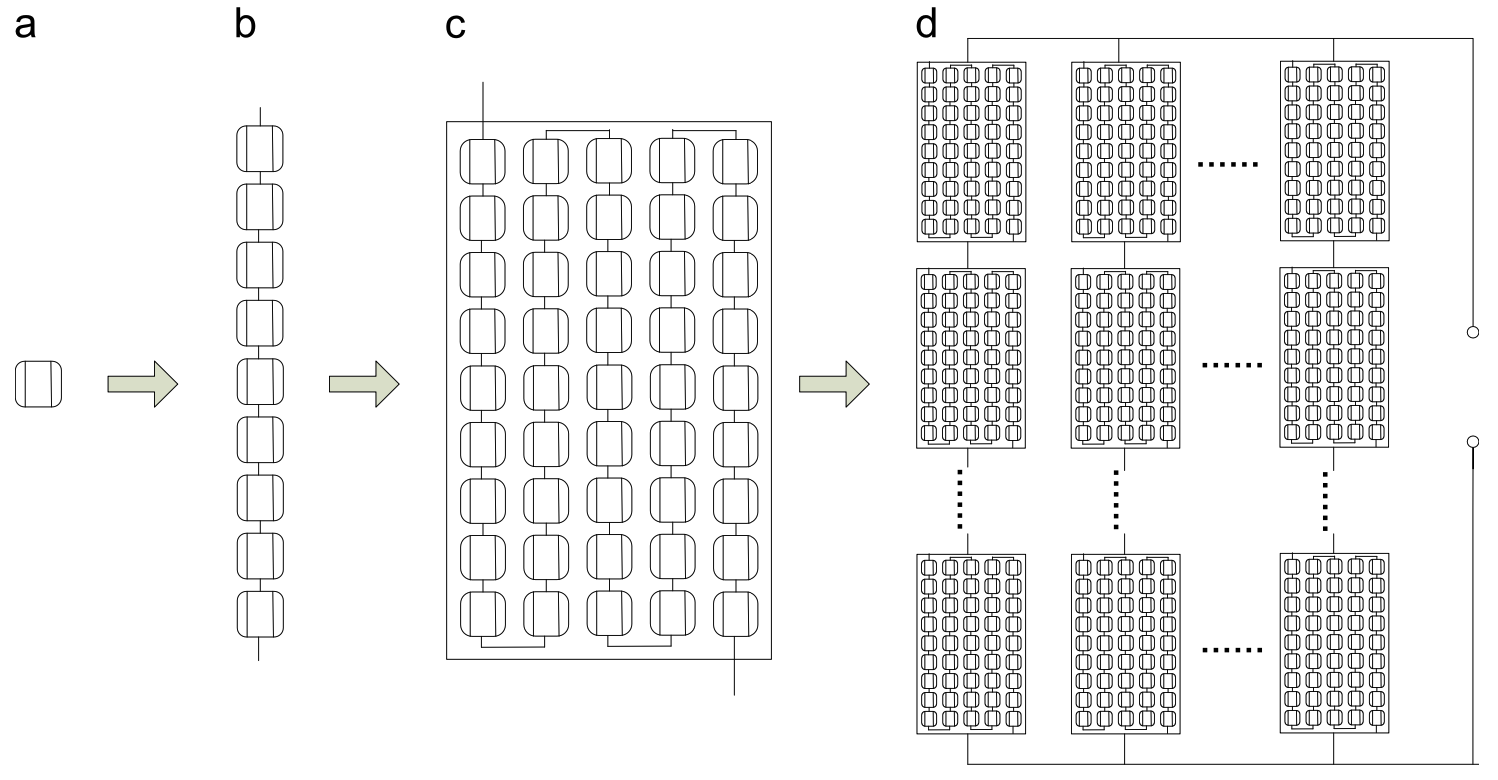
\includegraphics[scale=0.28]{PV_system_configuration_cell_module_array.png}
    \caption{\small Physical configuration of (a) PV cell, (b) cell series string, (c) module
             and (d) PV array \cite{Ma2014_1}.}
    \label{fig:PV_system_configuration_cell_module_array}
\end{figure}

\begin{figure}
    \centering
    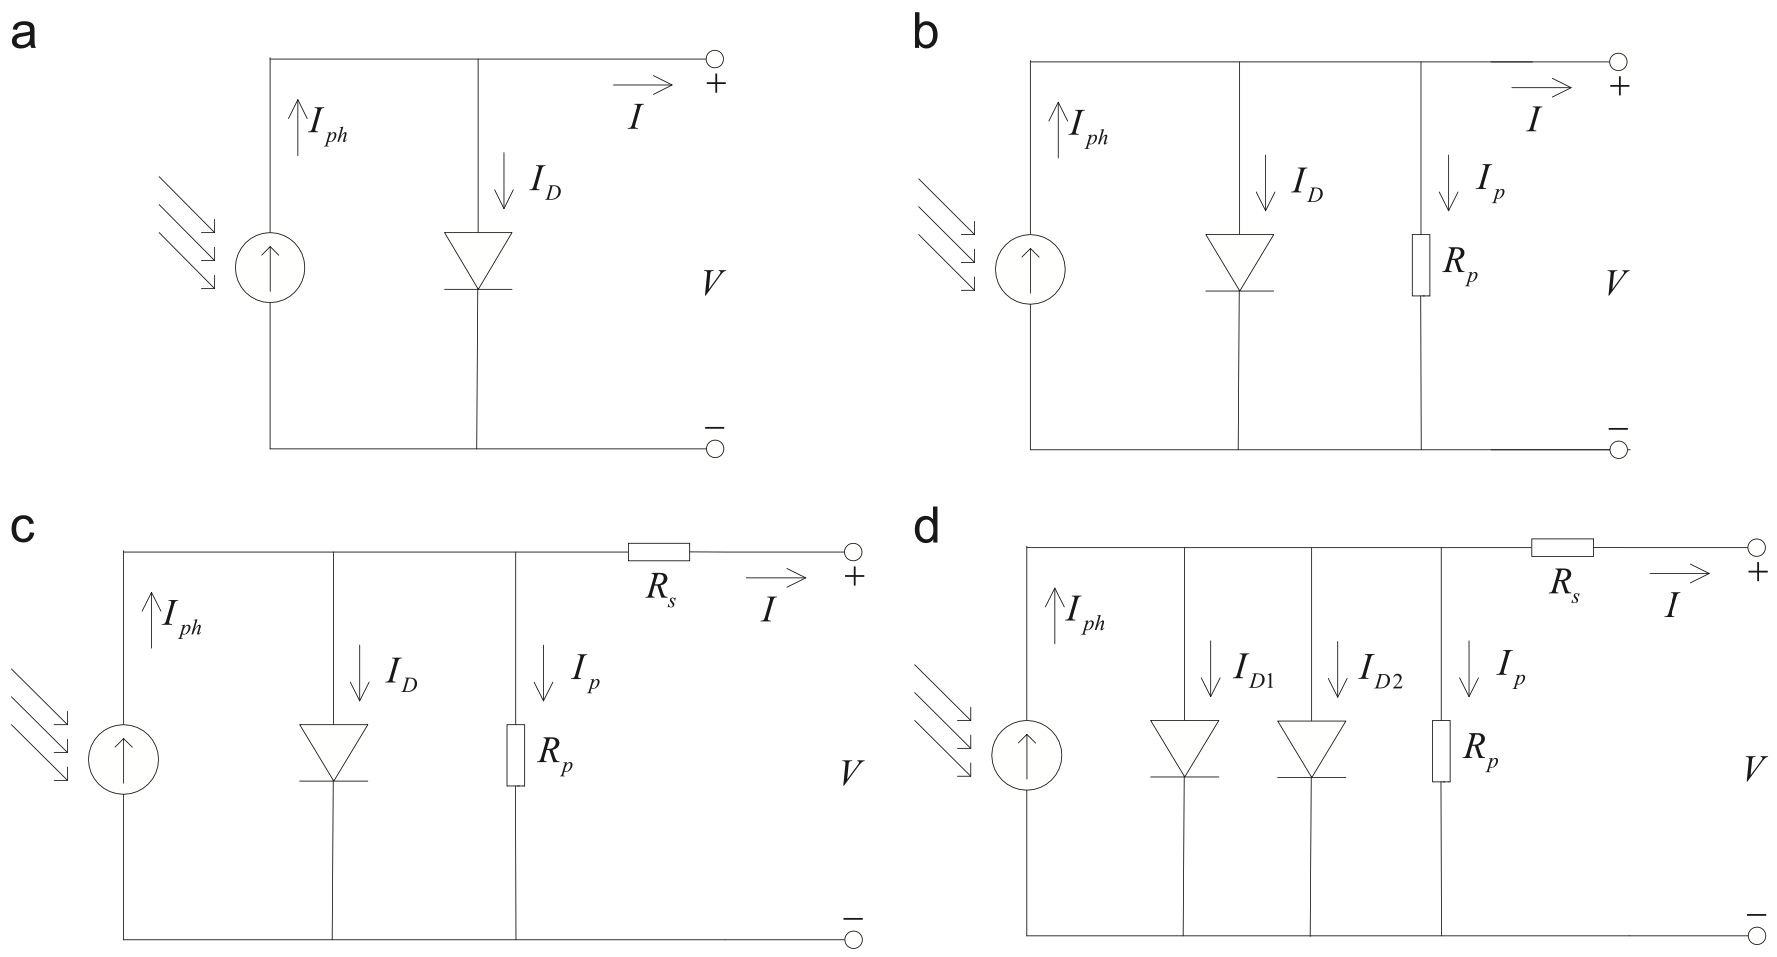
\includegraphics[scale=0.243]{Overview_equivalent_circuit_models.png}
    \caption{\small Equivalent PV cell electrical circuits: (a) ideal model,
        (b) one-diode with \(R_{\text{s}}\), (c) one-diode with \(R_{\text{s}} \text{ and } R_{\text{sh}}\),
        and (d) two-diode model \cite{Ma2014_1}.}
        \label{fig:Overview_equivalent_circuit_models}
\end{figure}

\label{sec:Background to physical models}
\subsection{Operating conditions}
As mentioned in the previous section, the parameters of the mathematical
models presented in Equations \ref{eq:Three_parameter_model},
\ref{eq:Four_parameter_model}, \ref{eq:Five_parameter_model}, and
\ref{eq:Seven_parameter_model} are either constant or depend on the
operating conditions. These conditions refer to the incident solar
radiation \(G_{\text{c}}\) and the cell temperature \(T\).
Section \ref{sec:Estimating in-plane irradiance} already discussed
how to estimate \(G_{\text{c}}\) impinging on an inclined plane from commonly
available global horizontal and diffuse horizontal irradiance data.
The cell temperature, often called the operating temperature, is
usually significantly higher than the ambient temperature \(T_{\text{amb}}\) (K)
and can also be estimated from commonly available meteorological data. The
models performing this estimation are known as thermal models. As noted in
\cite{Ma2014_1}, the operating temperature \(T\) in the models is assumed to be
equal to the temperature of the P-N junction of the solar cell, which is
encapsulated within a layered structure. This structure typically consists
of glass on the front side, which serves as a protective cover and allows
sunlight to penetrate, an encapsulant material, often ethylene-vinyl acetate
(EVA), which bonds the cell to the glass, and a backsheet. The backsheet
material is typically a polymer that provides electrical insulation and
environmental protection from moisture and physical damage.
Through heat transfer, it is reasonable to assume that the cell
temperature is influenced by factors such as incident solar
radiation, ambient temperature, wind speed, and wind direction.
Figure \ref{fig:Cell_temperature_and_irradiance_relationship} illustrates
the relationship between solar irradiance and the temperature
difference \(T - T_{\text{amb}}\) for different module types.
There appears to be a linear relationship in which the coefficient
depends on the module type. Ignoring other factors that influence
the relationship, such as module installation, wind speed, and
ambient humidity, a simplified estimation of the cell temperature
is given by:

\begin{figure}
    \centering
    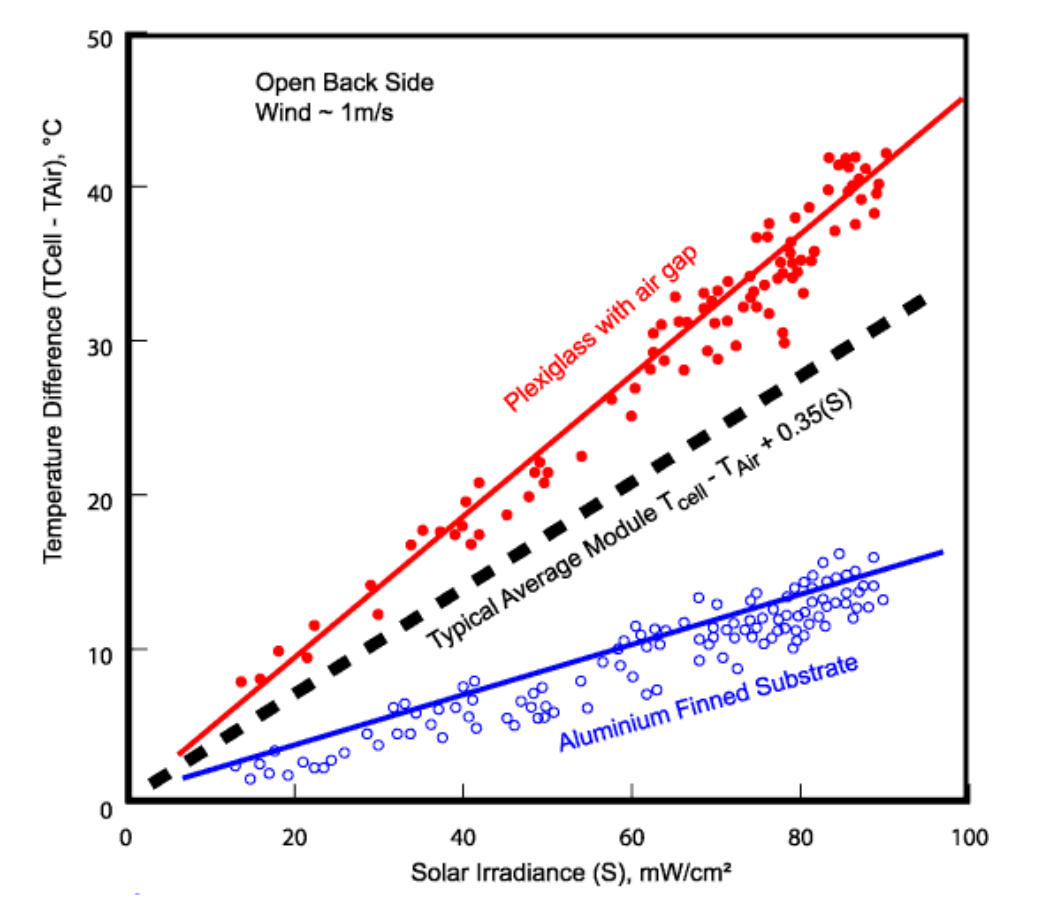
\includegraphics[scale=0.30]{Cell_temperature_and_irradiance_relationship.png}
    \caption{\small Relationship between solar irradiance \(S\) and temperature difference \(T-T_{\text{amb}}\) \cite{Ross1986}.}
    \label{fig:Cell_temperature_and_irradiance_relationship}
\end{figure}

\begin{equation}
    T = T_{\text{amb}} + G_{\text{c}} \; \frac{T_{\text{noct}} - 20}{800}
\end{equation}

\noindent
Here, \(T_{\text{noct}}\) (\si{\degreeCelsius}) refers to the cell temperature under Nominal Operating
Cell Temperature conditions \((T_{\text{amb,noct}} = 20 \si{\degreeCelsius}, \,
G_{\text{noct}} = 800 \, \si{\watt\per\meter\squared}, \text{ and wind speed } WS = 1 \,
\si{\meter\per\second})\) \cite[p. 302]{Hegedus2003}.
Sandia National Laboratories developed an empirically based
thermal model that has proven to be entirely adequate for
system engineering and design purposes. The model is described
by the set of equations:

\begin{align}
    T_{\text{m}} &= T_{\text{amb}} + G_{\text{c}} \exp \: \bigl(a + b \mathit{WS} \bigr)
    \label{eq:Cell_temperature_model_Sandia_module_temperature} \\
    T &= T_{\text{m}} + \frac{G_{\text{c}}}{G_{\text{ref}}} \Delta T
    \label{eq:Cell_temperature_model_Sandia_cell_temperature}
\end{align}

\noindent
As with the previous model, these equations establish a relationship between
the incident solar irradiance \(G_{\text{c}}\) and the cell temperature \(T\). However,
they additionally account for wind speed, module type, and installation
configuration. Equation \ref{eq:Cell_temperature_model_Sandia_module_temperature}
estimates the back-surface module temperature \(T_{\text{m}}\) from the wind speed \(WS\)
at a standard altitude of 10 meters and empirically determined coefficients \(a\) and \(b\).
Equation \ref{eq:Cell_temperature_model_Sandia_cell_temperature} relates the
back-surface module temperature \(T_{\text{m}}\) to the cell temperature \(T\) through a
simple relationship based on the assumption of one-dimensional thermal heat
conduction through the module materials behind the cell. The predetermined
coefficient \(\Delta T\) is the temperature difference between the cell and the
module back surface at an irradiance level of \(G_{\text{ref}} = 1000 \, \si{\watt\per\meter\squared}\).
Figure \ref{fig:Cell_temperature_Sandia_model_influence_of_wind_speed} illustrates
typical measured data recorded on six different days with nominally clear
conditions and a wide range of irradiance, wind speed, and wind direction,
indicating the derivation of a and b as a linear fit to the measured data.
Two mornings when the sun first illuminated the module are indicated as \say{heat up}.
In these periods of approximately 30 minutes, the fit of intercept \(a\) and slope \(b\)
may slightly underestimate the measurements \cite[p. 17ff]{Kratochvil2004}.
The coefficients recommended for different module types and installation
configurations are given in Table \ref{tab:Cell_temperature_thermal_coefficients}.
In this thesis, Sandia's thermal model is used to estimate the cell temperature,
as both the mounting configuration and module type are known. In applications
where such data is unavailable, the simpler thermal model may be used instead.

\begin{figure}
    \centering
    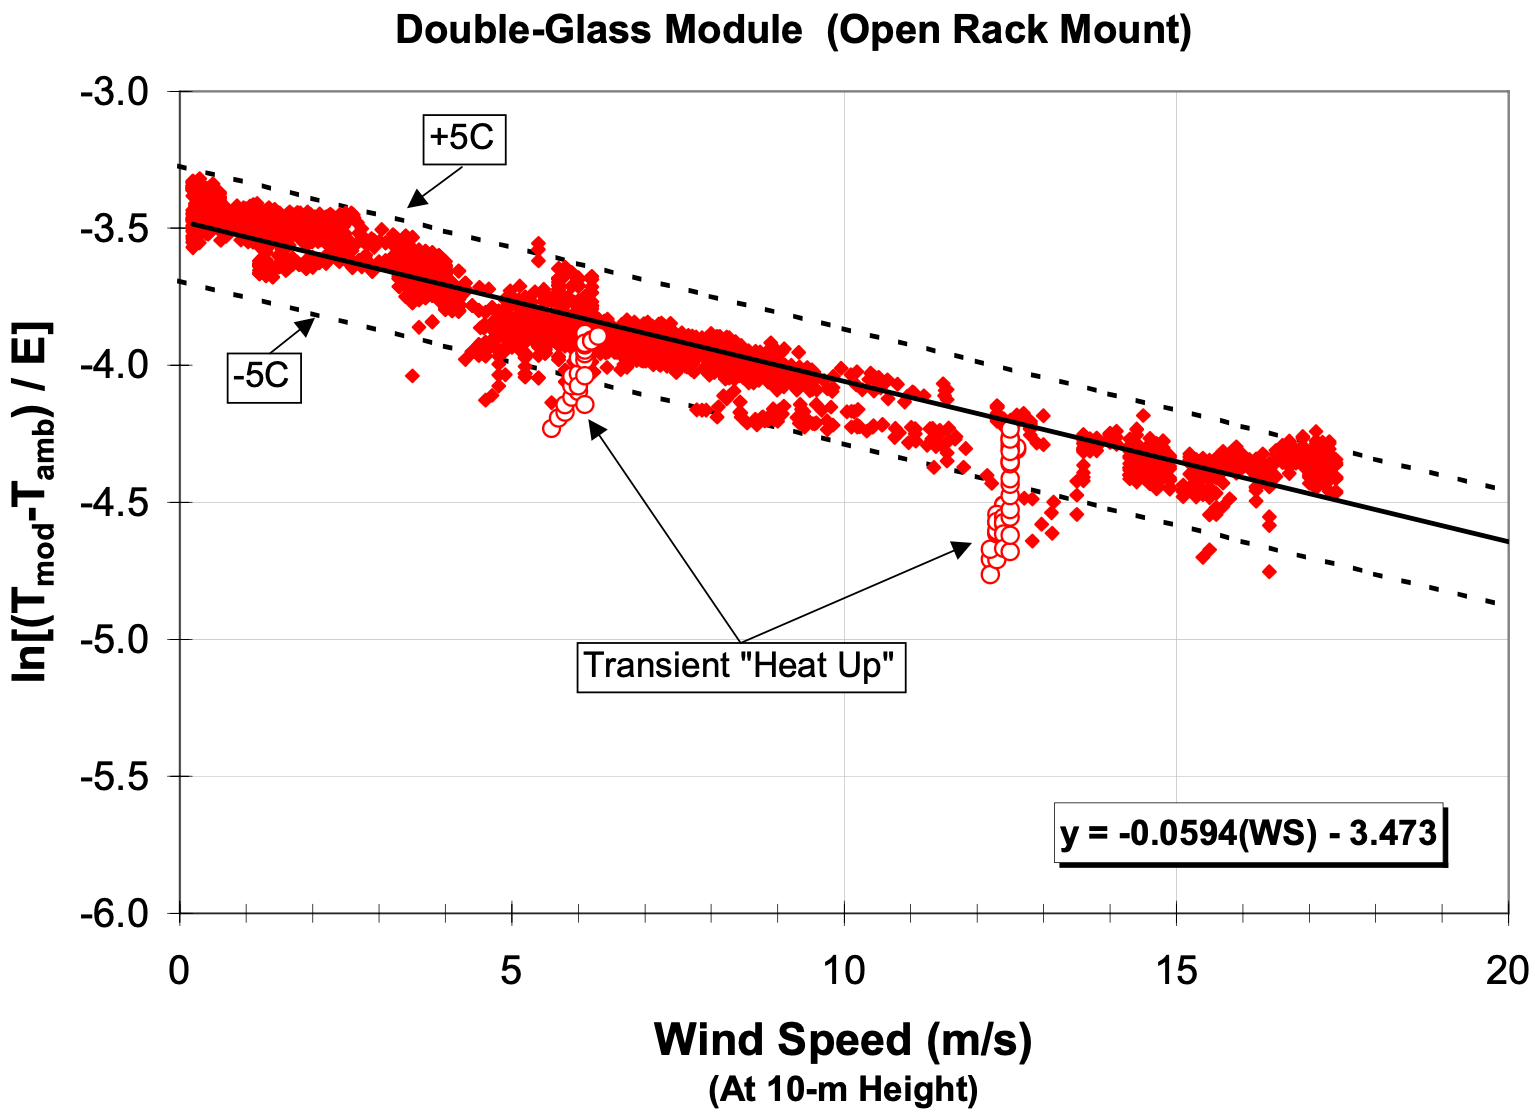
\includegraphics[scale=0.25]{Cell_temperature_Sandia_model_influence_of_wind_speed.png}
    \caption{\small Illustration of the derivation of the coefficients \(a\) and \(b\)
        in Sandia's thermal model \cite{Kratochvil2004}.}
    \label{fig:Cell_temperature_Sandia_model_influence_of_wind_speed}
\end{figure}

\begin{table}
    \centering
    \begin{tabular}{l l S S S}
        \toprule
        Module Type & Mount & {$a$} & {$b$} & \(\Delta T\) \\
        \midrule
        Glass/cell/glass         & Open rack         & -3.47 & -0.0594 & 3  \\
        Glass/cell/glass         & Close roof mount  & -2.98 & -0.0471 & 1  \\
        Glass/cell/polymer sheet & Open rack         & -3.56 & -0.0750 & 3  \\
        Glass/cell/polymer sheet & Insulated back    & -2.81 & -0.0455 & 0  \\
        Polymer/thin-film/steel  & Open rack         & -3.58 & -0.1130 & 3  \\
        22X Linear Concentrator  & Tracker           & -3.23 & -.1300  & 13 \\
        \bottomrule
    \end{tabular}
    \caption{\small Thermal coefficients for various module types and mounting configurations 
        \cite{Kratochvil2004}.}
    \label{tab:Cell_temperature_thermal_coefficients}
\end{table}

\label{sec:Operating_conditions}
\subsection{Current-voltage characteristic and standard test conditions}
\label{sec:I-V characteristic curve}
The current-voltage characteristic is fundamental to understanding PV
device performance. It is a graphical representation of the relationship
between the current \(I\) and voltage \(V\) of a PV device and is often
abbreviated as the I-V characteristic or I-V curve.
Figure \ref{fig:Surfclub_IV_and_PV_curve_at_STC} shows the I-V characteristic of
a 330-watt photovoltaic module alongside its corresponding power-voltage
(P-V) curve under Standard Test Conditions. Standard Test Conditions (STC),
sometimes also referred to as Standard Rating Conditions (SRC), denote
an industry-standard set of operating conditions under which manufacturers
test the performance of their photovoltaic modules and report the results
in datasheets. These conditions specify a cell temperature of \(T = 298.15 \, \si{\kelvin}\)
and an incident irradiance of \(G_{\text{ref}} = 1000 \, \si{\watt\per\meter\squared}\) with an
air mass 1.5 solar spectrum. The figure also highlights three
important points of the I-V graph:

\begin{itemize}
    \item the open circuit point \((V = V_{oc}, I = 0,)\): The intersection with the voltage axis when
        the current is zero, representing the maximum voltage the module can produce under open-circuit conditions.
    \item the short circuit point \((V = 0, I = I_{sc})\): The intersection with the current axis when
        the voltage is zero, representing the maximum current the module can produce under short-circuit conditions.
    \item the maximum power point \((V = V_{mp}, I = I_{mp})\): The point for which the product of
        the current \(I\) and voltage \(V\) is maximized. The maximum power is given by \(P_{mp} = V_{mp} I_{mp}\).
\end{itemize}

Most modern PV module datasheets provide information on
these three points under Standard Test Conditions (STC),
and in some cases, even include the entire I-V curve. As
will be seen in Section \ref{sec:Five_parameter_model},
which presents the five-parameter model used in this thesis,
this information, along with other data from the module
datasheet, is used to calculate the model parameters.

As might be expected, only a single point from
the simulated I-V characteristic is needed to formulate a
prediction for a PV device. Ideally, this point corresponds
to the true operating point of the device, that is, the point
on the I-V curve at which the PV device operates at a
given instant. The last section of this chapter will
demonstrate how this point is chosen under certain
assumptions appropriate for PV system modeling.

All mathematical models presented in Section
\ref{sec:Background to physical models}, except for the
ideal model, are implicit, meaning they cannot be solved
explicitly for either \(I\) or \(V\). In these cases, the I-V
characteristic can be interpreted as the zero-level
set \(f_{\kappa}(V, I) = 0\)  of an appropriately defined
function \(f_{\kappa}: \mathbb{R}^2 \rightarrow \mathbb{R}\),
constrained to the upper right quadrant of the I-V plane.
The set \(\kappa\) represents the model parameters, some of
which are constant, while others depend on the operating
conditions as mentioned in Section \ref{sec:Background to physical models}.

\begin{figure}[H]
    \centering
    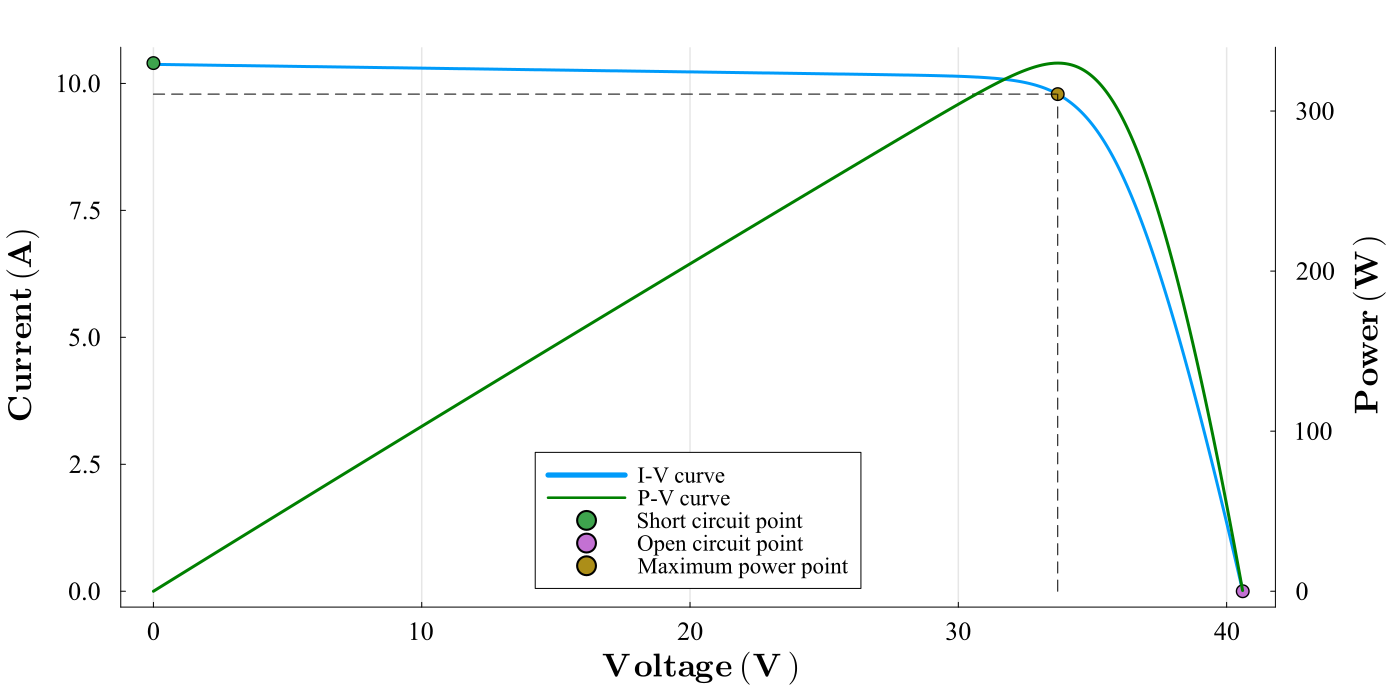
\includegraphics[scale=0.3]{Surfclub_IV_and_PV_curve_at_STC.png}
    \caption{\small Current-voltage characteristic and corresponding power-voltage curves of a photovoltaic module at STC.}
    \label{fig:Surfclub_IV_and_PV_curve_at_STC}
\end{figure}

\subsection{An improved five-parameter model}

This section introduces a physical model capable of analytically describing
the current-voltage characteristic of photovoltaic (PV) modules under generic
operating conditions. The model is an improved version of the five-parameter
model and was first proposed in \cite{LoBrano}. Two years later,
two of the authors published a second paper \cite{Orioli} on the same model,
providing a procedure to calculate the model parameters for monocrystalline
and polycrystalline modules, including those based on the Sanyo HIT
(heterojunction with intrinsic thin layer) technology, requiring slightly
less input data. The model is formulated, and a procedure is presented to
determine its parameters using the information provided in both papers,
ensuring optimal use with minimal input data for all types of photovoltaic
modules.

The analytical expression of the I-V characteristic curve in the
considered papers has the form:

\begin{align}
    I = \; &\alpha_{\text{G}}I_{\text{L}}(T) - I_{0}(\alpha_{\text{G}}, T)\Biggl[\exp\biggl(\frac{\alpha_{\text{G}}(V + KI(T - T_{\text{ref}}))+IR_{\text{s}}}{\alpha_{\text{G}}nT}\biggr) - 1\Biggr] \nonumber \\
                       &- \frac{\alpha_{\text{G}}(V + KI(T - T_{\text{ref}}))+IR_{\text{s}}}{R_{\text{sh}}}
    \label{eq:Orioli_IV_curve_governing_equation}
\end{align}

\noindent
Here, \(\alpha_{\text{G}} = G_{\text{c}} / G_{\text{ref}}\) denotes the ratio between
the incident solar irradiance \(G_{c}\) on the module and the irradiance at STC
\(G_{\text{ref}} = 1000 \, \si{\watt\per\meter\squared}\) \footnote{The subscript \say{ref} is used to denote the values at STC}
and \(K\) is a thermal correction
factor. The set of parameters \(\kappa\), as introduced in Section
\ref{sec:I-V characteristic curve}, is given by:

\begin{equation}
    \kappa = \{R_{\text{s}}, R_{\text{sh}}, n, K, I_{\text{L}}, I_{0}\}
\end{equation}

\noindent
Here, \(R_{\text{s}}\), \(R_{\text{sh}}\), \(n\) and \(K\) are constants, while, as indicated by Equation
\ref{eq:Orioli_IV_curve_governing_equation}, \(I_{\text{L}}\) and \(I_{0}\) depend on the
generic operating conditions. The parameter determination can be divided into two steps:
(i) derivation of all constants in \(\kappa\) and of \(I_{\text{L}}\) and \(I_{0}\) at STC and (ii)
determination of \(I_{\text{L}}\) and \(I_{0}\) at generic operating conditions, which require the knowledge
of the values in step (i). After these steps, the only unknowns in Equation \ref{eq:Orioli_IV_curve_governing_equation}
are the current \(I\) and voltage \(V\), and the solution set can be determined. The generic
operating conditions \(\alpha_{\text{G}}\) and \(T\) are known prior to the parameter determination
and therefore not considered parameters.

The values \(I_{\text{L,ref}}\), \(I_{\text{0,ref}}\), \(n\), \(R_{\text{s}}\) and \(R_{\text{sh}}\)
in step (i) are determined using the procedure described in \cite[p. 1362f]{LoBrano}.
It uses the following points at STC that can be obtained from the tabular
performance data commonly provided by manufacturers: open-circuit voltage
\(V_{\text{oc,ref}}\), short-circuit current \(I_{\text{sc,ref}}\), and the maximum
power point \((V_{\text{mp,ref}}, I_{\text{mp,ref}})\).

\begin{itemize}
    \item short circuit point: \(V = 0, I = I_{sc,ref}\)
    \begin{equation}
        I_{\text{sc,ref}} = I_{\text{L,ref}} - I_{\text{0,ref}} \Biggl[ \exp\biggl(\frac{I_{\text{sc,ref}}R_{\text{s}}}{nT_{\text{ref}}}\biggr) - 1 \Biggr] - \frac{I_{\text{sc,ref}}R_{\text{s}}}{R_{\text{sh}}}
        \label{eq:IV_at_short_circuit_point_at_SRC}
    \end{equation}
    \item open circuit point: \(V = V_{\text{oc,ref}}, I = 0\)
    \begin{equation}
        0 = I_{\text{L,ref}} - I_{\text{0,ref}} \Biggl[ \exp\biggl(\frac{V_{\text{oc,ref}}}{nT_{\text{ref}}}\biggr) - 1 \Biggr] - \frac{V_{\text{oc,ref}}}{R_{\text{sh}}}
        \label{eq:IV_at_open_circuit_point_at_SRC}
    \end{equation}
    \item maximum power point: \(V = V_{\text{mp,ref}}, I = I_{\text{mp,ref}}\)
    \begin{equation}
        I_{\text{mp,ref}} = I_{\text{L,ref}} - I_{\text{0,ref}} \Biggl[ \exp\biggl(\frac{V_{\text{mp,ref}} + I_{\text{mp,ref}}R_{\text{s}}}{nT_{\text{ref}}}\biggr) - 1 \Biggr] - \frac{V_{\text{mp,ref}} + I_{\text{mp,ref}}R_{\text{s}}}{R_{\text{sh}}}
        \label{eq:IV_at_maximum_power_point_at_SRC}
    \end{equation}
    \item derivative at the short circuit point
    \begin{equation}
        \left.\frac{dI}{dV}\right|_{V = 0, I = I_{\text{sc,ref}}} = - \frac{\frac{I_{\text{0,ref}}}{nT_{\text{ref}}} \exp\bigl(\frac{I_{\text{sc,ref}}R_{\text{s}}}{nT_{\text{ref}}}\bigr) + \frac{1}{R_{\text{sh}}}}{1 + R_{\text{s}}\Bigl[ \frac{I_{\text{0,ref}}}{nT_{\text{ref}}} \exp\bigl(\frac{I_{\text{sc,ref}}R_{\text{s}}}{nT_{\text{ref}}}\bigr) + \frac{1}{R_{\text{sh}}} \Bigr]} = -\frac{1}{R_{\text{sho}}}
        \label{eq:IV_derivative_at_short_circuit_point_at_SRC}
    \end{equation}
    \item derivative at the open circuit point
    \begin{equation}
        \left.\frac{dI}{dV}\right|_{ V = V_{\text{oc,ref}}, I = 0} = - \frac{\frac{I_{\text{0,ref}}}{nT_{\text{ref}}} \exp\bigl(\frac{V_{\text{oc,ref}}}{nT_{\text{ref}}}\bigr) + \frac{1}{R_{\text{sh}}}}{1 + R_{\text{s}}\Bigl[ \frac{I_{\text{0,ref}}}{nT_{\text{ref}}} \exp\bigl(\frac{V_{\text{oc,ref}}}{nT_{\text{ref}}}\bigr) + \frac{1}{R_{\text{sh}}} \Bigr]} = -\frac{1}{R_{\text{so}}}
        \label{eq:IV_derivative_at_open_circuit_point_at_SRC}
    \end{equation}
\end{itemize}

\noindent
Equations \ref{eq:IV_at_short_circuit_point_at_SRC}, \ref{eq:IV_at_open_circuit_point_at_SRC},
and \ref{eq:IV_at_maximum_power_point_at_SRC} are obtained by evaluating Equation
\ref{eq:Orioli_IV_curve_governing_equation} at the short-circuit, open-circuit,
and maximum power points, respectively. Equations
\ref{eq:IV_derivative_at_short_circuit_point_at_SRC} and \ref{eq:IV_derivative_at_open_circuit_point_at_SRC}
set the derivative of Equation \ref{eq:Orioli_IV_curve_governing_equation}
at the short-circuit and open-circuit points equal to the slope of the
characteristic curve at these points. \(R_{\text{sho}}\) and \(R_{\text{so}}\) denote
the absolute values of the reciprocals of the slopes of the I-V curve at STC
at the respective points. These values are referred to as
reciprocals of slopes in both \cite{LoBrano} and \cite{Orioli}.
The implicit formulation of Equation \ref{eq:Orioli_IV_curve_governing_equation}
does not directly allow differentiation with respect to V to derive Equations
\ref{eq:IV_derivative_at_short_circuit_point_at_SRC} and \ref{eq:IV_derivative_at_open_circuit_point_at_SRC}.
These equations are derived next, noting that this discussion is not
included in \cite{LoBrano} and \cite{Orioli}. After subtracting the photocurrent
from both sides of Equation \ref{eq:Orioli_IV_curve_governing_equation}, the
equation can be compactly written in the form \(f(V, I) = 0\) for an appropriately
chosen function \(f: \mathbb{R}^2 \rightarrow \mathbb{R}\), as indicated in Section
\ref{sec:I-V characteristic curve}. This function is continuously differentiable,
and the slopes of the zero-level set at the short-circuit and open-circuit
points can be derived as the slopes of the intersections of the linear
approximations of \(f\) at the respective points with the I-V plane.
This approach leads to the following set of equations:

\begin{align}
    0 &= f(x) + \nabla f(x)^Th \nonumber \\
      &= f(V,I) + \partial_{V}f(V,I)h_{1} + \partial_{I}f(V,I)h_{2} \nonumber \\
    \Leftrightarrow h_2 &= -\frac{f(V,I)}{\partial_{I}f(V,I)} - \frac{\partial_{V}f(V,I)}{\partial_{I}f(V,I)}h_{1}
    \label{eq:IV_derivation_of_slopes_of_reciprocals}
\end{align}

\noindent
The above derivation starts by calculating the intersection of the linear approximation
of \(f\) at an arbitrary point \(x = (V, I)\) with the I-V plane. It is then
solved for \(h_{2}\), expressing the intersection as a linear function of \(h_{1}\).
Evaluating the slope of Equation \ref{eq:IV_derivation_of_slopes_of_reciprocals} at
the respective points yields the left-hand sides of Equations
\ref{eq:IV_derivative_at_short_circuit_point_at_SRC} and \ref{eq:IV_derivative_at_open_circuit_point_at_SRC}:

\begin{align}
    \left.\frac{dI}{dV}\right|_{V = 0, I = I_{\text{sc,ref}}} &= - \frac{\partial_{V}f(0,I_{\text{sc,ref}})}{\partial_{I}f(0,I_{\text{sc,ref}})} \\
    \left.\frac{dI}{dV}\right|_{ V = V_{\text{oc,ref}}, I = 0} &= - \frac{\partial_{V}f(V_{\text{oc,ref}},0)}{\partial_{I}f(V_{\text{oc,ref}},0)}
\end{align}

Sometimes, graphical data needed to estimate \(R_{\text{so}}\) and \(R_{\text{sho}}\) is
lacking. To account for this, the authors of \cite{Orioli} provided two relations
that reasonably represent these values:

\begin{align}
    R_{\text{so}} &= C_{\text{so}} \: \frac{V_{\text{oc,ref}}}{I_{\text{sc,ref}}}
    \label{eq:Estimation_of_Rso} \\
    R_{\text{sho}} &= C_{\text{sho}} \: \frac{V_{\text{oc,ref}}}{I_{\text{sc,ref}}}
    \label{eq:Estimation_of_Rsho}
\end{align}

\noindent
with \(C_{\text{so}} = 0.11175\) and \(C_{\text{sho}} = 34.49692\) for monocrystalline and polycrystalline
modules. Suitable values for PV panels based on the Sanyo HIT (heterojunction with intrinsic
thin layer) technology are \(C_{\text{so}} = 0.16129\) and \(C_{\text{sho}} = 124.48114\). The authors
established these relations by surveying 144 PV modules from 30 different manufacturers,
whose datasheets were available on the internet \cite[p. 1164]{Orioli}. Figure
\ref{fig:Orioli_estimation_of_Rso_and_Rsho} illustrates the graphical evaluation
of these values, which can also be used when graphical data is present.

\begin{figure}[H]
    \centering
    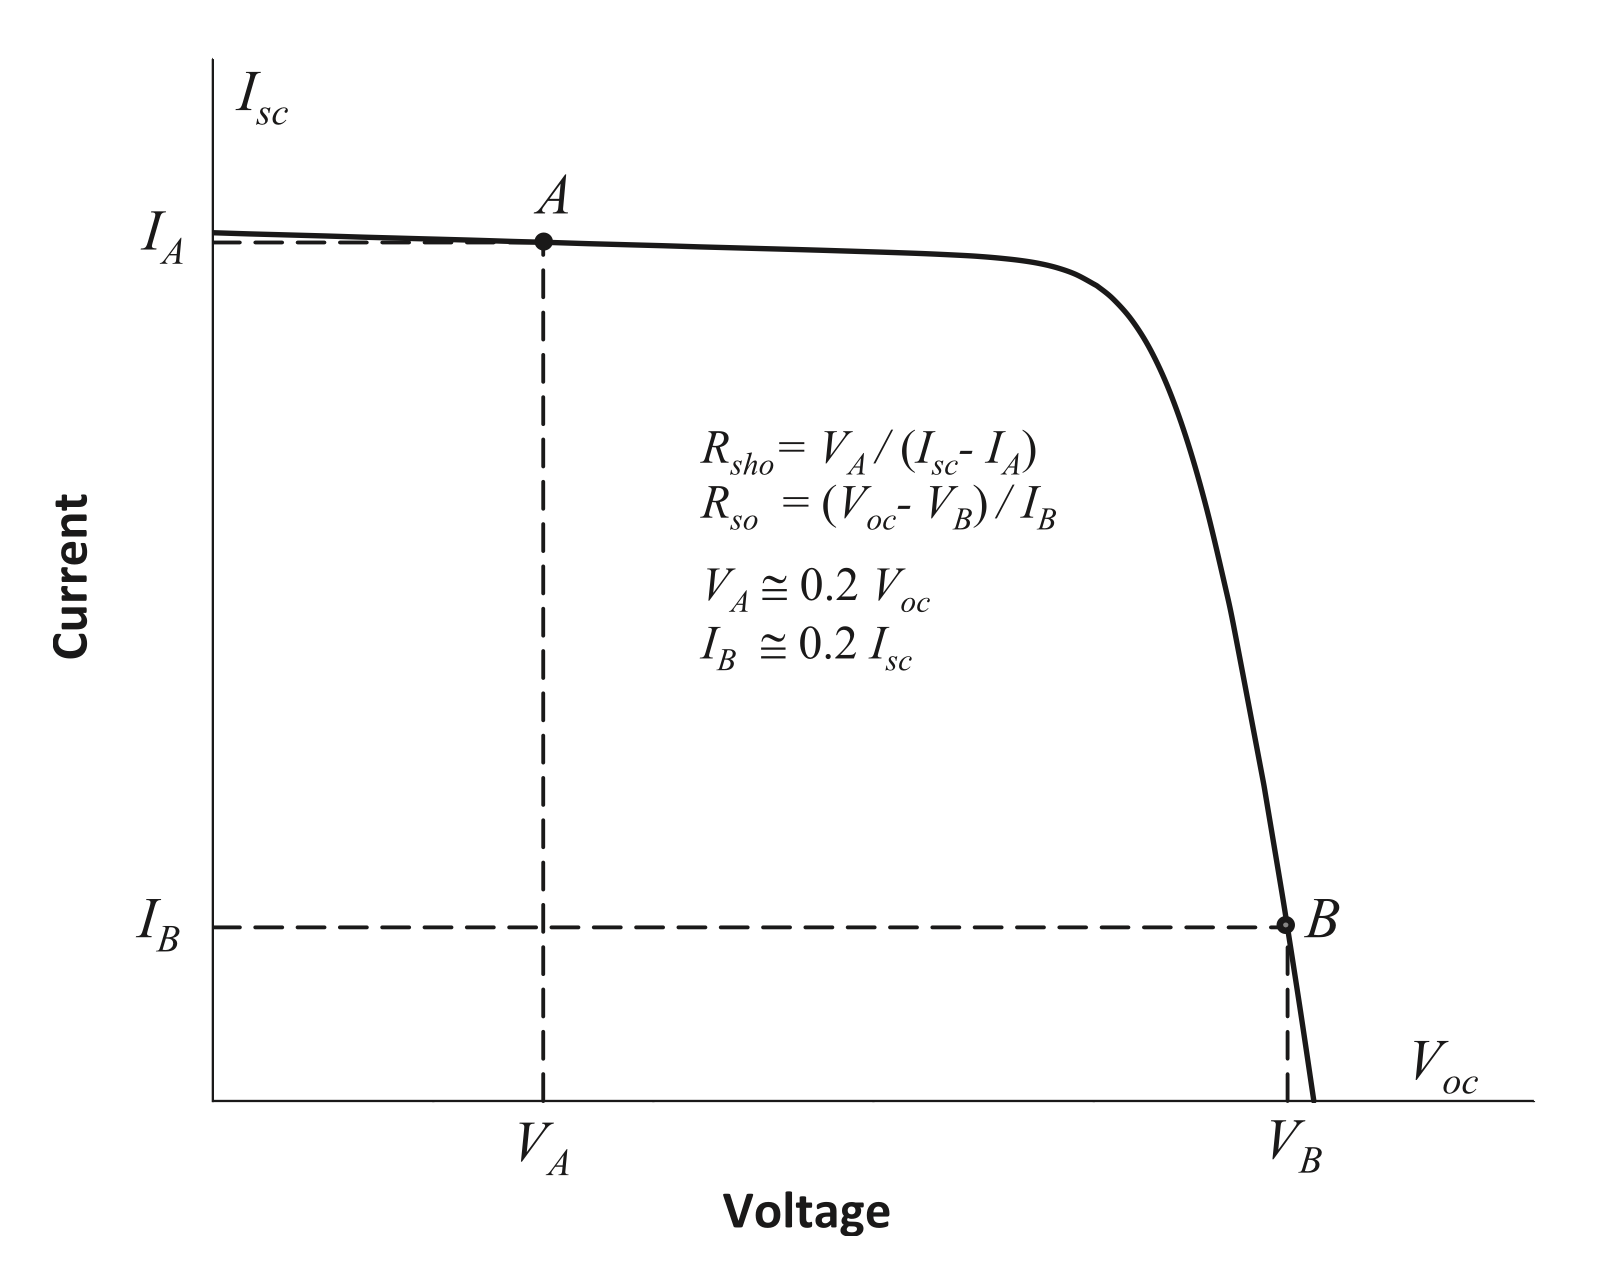
\includegraphics[scale=0.20]{Orioli_estimation_of_Rso_and_Rsho.png}
    \caption{\small Graphical evaluation of \(R_{\text{so}}\) and \(R_{\text{sho}}\) in the I-V characteristic at STC \cite{Orioli}.}
    \label{fig:Orioli_estimation_of_Rso_and_Rsho}
\end{figure}

The solution of Equations \ref{eq:IV_at_short_circuit_point_at_SRC} to
\ref{eq:IV_derivative_at_open_circuit_point_at_SRC} was initially
attempted using software like Mathematica and MATLAB. However, the
authors could not achieve a valid solution and proposed a numerical
algorithm instead, which consists of a double trial-and-error
process with the second nested within the first. The process starts
with an initial guess of \(R_{\text{s}}\) and \(n\), and the following conditions:

\begin{equation}
    I_{\text{L,ref}} = I_{\text{sc,ref}} \qquad R_{\text{sh}} = R_{\text{sho}}
    \label{eq:LoBrano_Orioli_initial_conditions}
\end{equation}

\noindent
These conditions are obtained from Equations \ref{eq:IV_at_short_circuit_point_at_SRC}
and \ref{eq:IV_derivative_at_short_circuit_point_at_SRC} under the commonly satisfied
assumptions \cite[p. 1362]{LoBrano}:

\begin{equation}
    R_{\text{s}} \ll R_{\text{sho}} \qquad \frac{I_{\text{0,ref}}}{nT_{\text{ref}}}\exp\bigl(\frac{I_{\text{sc,ref}}R_{\text{s}}}{nT_{\text{ref}}}\bigr) \ll \frac{1}{R_{\text{sh}}}
\end{equation}

\noindent
The inner trial evaluates \(I_{0}\), \(I_{\text{L}}\), \(R_{\text{sh}}\) and \(n\) in
sequence using Equations \ref{eq:IV_at_maximum_power_point_at_SRC},
\ref{eq:IV_at_short_circuit_point_at_SRC}, \ref{eq:IV_derivative_at_short_circuit_point_at_SRC},
and \ref{eq:IV_at_open_circuit_point_at_SRC} until convergence of n is
achieved with the desired accuracy. The outer trial recalculates \(R_{\text{s}}\)
with Equation \ref{eq:IV_derivative_at_open_circuit_point_at_SRC} after
each inner trial and repeats the process until convergence of \(R_{\text{s}}\) is
achieved with the desired accuracy. In this way, the five equations are
solved in a non-approximate form because no simplifications are used.
It is worth noting that the procedure in \cite[p. 1163f]{Orioli} to determine
the values in step (i) uses the positions in Equation \ref{eq:LoBrano_Orioli_initial_conditions}
as parameters and determines the remaining values \(I_{\text{0,ref}}\), \(n\) and \(R_{\text{s}}\)
in a single trial-and-error process using Equations
\ref{eq:IV_at_open_circuit_point_at_SRC}, \ref{eq:IV_at_maximum_power_point_at_SRC},
and \ref{eq:IV_derivative_at_open_circuit_point_at_SRC}, leading to a satisfactory
approximate set of parameters.

The thermal correction factor K has the effect of shifting the I-V curve at irradiance
\(G_{\text{ref}}\) along the voltage axis to better fit the characteristics provided by the
manufacturer at temperatures \(T^*\) different from \(T_{\text{ref}}\) \cite[p. 1365]{LoBrano}.
The procedure described in \cite{Orioli} is presented, which does not require knowledge
of the maximum power point at a temperature \(T = T^*\) different from \(T_{\text{ref}}\),
unlike the method presented in \cite{LoBrano}. The parameter \(K\) will be determined for
a chosen temperature \(T^*\) such that the corresponding maximum power at reference
irradiance equals the value of the maximum power obtained by:

\begin{equation}
    P_{\text{mp}}^* = P_{\text{mp,ref}} (1 + \frac{\mu_{P_{\text{mp}}}}{100} (T^* - T_{\text{ref}}))
    \label{eq:Maximum_power_in_correspondence_to_temperature_coefficient}
\end{equation}

\noindent
where \(\mu_{P_{\text{mp}}}\) is the temperature coefficient of the
maximum power point provided by the manufacturer. The temperature \(T^*\)
should be chosen by considering the maximum or minimum expected operating
temperature for the PV module \cite[p. 1365]{LoBrano}.
It is evident that the problem of finding the maximum power on the I-V
curve in the described setting can equivalently be formulated as:

\begin{alignat}{2}
    & \max_{V_{\text{d}}, I}    & \quad & V_{\text{d}} I - I^2 [R_{\text{s}} + K(T^* - T_{\text{ref}})]
    \label{eq:Parameter_K_optimization_problem_objective} \\
    & \text{subject to} & \quad & I - I_{\text{L}}^* + I_{0}^* \left[\exp\left(\frac{V_{\text{d}}}{nT^*}\right) - 1\right] + \frac{V_{\text{d}}}{R_{\text{sh}}} = 0
    \label{eq:Parameter_K_optimization_problem_constraint}
\end{alignat}

\noindent
Here, \(I_{\text{L}}^*\) and \(I_{0}^*\) are the photocurrent and reverse saturation current
at the considered operating conditions, and the substitution \(V_{\text{d}} = V + KI(T^* - T_{\text{ref}}) +IR_{\text{s}}\)
represents the voltage across the diode \cite[p. 1166]{Orioli}. Instead of
finding \(K\) through a trial-and-error process, wherein each iteration compares
the calculated maximum power point for the given \(K\) is compared with \(P_{\text{mp}}^*\), the
authors propose a numerical procedure based on the method of Lagrange
multipliers. The idea is to find a Karush-Kuhn-Tucker (KKT) point in
each iteration of the equivalent equality-constrained optimization
problem and compare the corresponding maximum power of the original
problem with \(P_{\text{mp}}^*\)  until convergence of \(K\) is achieved
with the desired accuracy. The Lagrange multiplier rule of the equality
contraint optimization problem takes the form:

\begin{align}
    I + \lambda \Biggl[ \frac{I_{0}^*}{nT} \exp \Biggl( \frac{V_{\text{d}}}{nT^*}\Biggr) + \frac{1}{R_{\text{sh}}}\Biggr] &= 0
    \label{eq:Parameter_K_optimization_problem_multiplier_rule_dVd} \\
    V_{\text{d}} - 2I[R_{\text{s}} + K(T-T_{\text{ref}})] + \lambda &= 0 
    \label{eq:Parameter_K_optimization_problem_multiplier_rule_dI}
\end{align}

\noindent
where \(\lambda\) denotes the Lagrange multiplier.
By expressing \(\lambda\) from Equation \ref{eq:Parameter_K_optimization_problem_multiplier_rule_dI}
and substituting it into Equation \ref{eq:Parameter_K_optimization_problem_multiplier_rule_dVd},
setting the result equal to the constraint in Equation \ref{eq:Parameter_K_optimization_problem_constraint},
and solving for \(V_{\text{d}}\) in the exponential term, the following expression is obtained:

\begin{equation}
    V_{\text{d}} = nT^* \Biggl[ \ln \Biggl( \frac{R_{\text{sh}}(I_{\text{L}}^* + I_{0}^*) - 2(V_{\text{d}} - I\tilde{R}_{\text{s}})}{R_{\text{sh}}(V_{\text{d}} - 2I\tilde{R}_{\text{s}})} \Biggr)- \ln \Biggl( I_{0}^* \Bigl( \frac{1}{nT^*} + \frac{1}{V_{\text{d}} - 2I\tilde{R}_{\text{s}}} \Bigr) \Biggr)\Biggr]
    \label{eq:Parameter_K_optimization_problem_fixpoint}
\end{equation}

\noindent
where \(\tilde{R}_{\text{s}} = R_{\text{s}} + K(T^* - T_{\text{ref}})\). Each inner loop of
finding \(K\) starts by initializing:

\begin{equation}
    V_{\text{d}} = -nT^* \ln\biggl( \frac{I_{0}^*}{nT^*} \biggr)
\end{equation}

\noindent
The procedure iteratively evaluates Equations \ref{eq:Parameter_K_optimization_problem_multiplier_rule_dVd}
and \ref{eq:Parameter_K_optimization_problem_fixpoint} in sequence, for six iterations as
suggested by \cite{Orioli}, to obtain a stable value of \(V_{\text{d}}\), denoted \(V_{\text{d,mp}}\). The
corresponding maximum power of the original problem, needed for comparison with
\(P_{\text{mp}}^{*}\), is derived from the equality constraint
(Equation \ref{eq:Parameter_K_optimization_problem_constraint}) and the substitution:

\begin{align}
    I_{\text{mp}} &= I_{\text{L}}^* - I_{0}^* \left[\exp\left(\frac{V_{\text{d,mp}}}{nT^*}\right) - 1\right] - \frac{V_{\text{d,mp}}}{R_{\text{sh}}} = 0 \\
    V_{\text{mp}} &= V_{\text{d,mp}} - KI(T-T_{\text{ref}}) - IR_{\text{s}}
\end{align}

\noindent
The authors of \cite{Orioli} used the slightly different objective function
\(V_{\text{d}}I - I^2R_{\text{s}}\) in Equation \ref{eq:Parameter_K_optimization_problem_objective},
which does not yield an equivalent problem. Consequently, the above procedure
differs from the one described in their paper. As can be seen from the steps
above, the original procedure uses \(R_{\text{s}}\) instead of \(\tilde{R}_{\text{s}}\) in Equation
\ref{eq:Parameter_K_optimization_problem_fixpoint}. Both
procedures have been compared by applying them to the four investigated PV modules in \cite{Orioli},
using a trial-and-error process in which the maximum power is found through
a nonlinear solver. The results are presented in Table \ref{tab:Parameter_K_procedure_comparision}.
As expected, using the objective function of the equivalent problem leads
to the same values of \(K\), confirmed by a difference of zero in the first
four rows. However, the objective function used in \cite{Orioli} leads to
small deviations, as seen in the last four rows. The authors do not
comment on this. Since the parameter \(K\) is a constant that only needs to
be calculated once, and its computation using a non-linear solver is fast,
this method may be preferred over the presented numerical procedure. 

\begin{table}
    \centering
    \resizebox{\columnwidth}{!}{
        \begin{tabular}{lll}
            \toprule
            Objective function & PV module & Difference in calculated K \\
            \midrule
            \(V_{\text{d}}I - I^2(R_{\text{s}} + K[T^*-T_{\text{ref}}])\) & Gruposolar GS601456P-218 & 0 \\
             & Kyocera KC175GHT-2  & 0 \\
             & Sanyo HIP-230 HDE1 & 0 \\
             & Shell SP75 & 0 \\
            \midrule
            \(V_{\text{d}}I - I^2R_{\text{s}}\) & Gruposolar GS601456P-218 & \(2.17933 \times 10^{-4}\) \\
             & Kyocera KC175GHT-2  & \(3.28 \times 10^{-7}\) \\
             & Sanyo HIP-230 HDE1 & \(2.15202 \times 10^{-4}\) \\
             & Shell SP75 & \(3.58 \times 10^{-6}\) \\
            \bottomrule
        \end{tabular}
    }
    \caption{\small Results of comparision between the procedure of calculating the parameter \(K\) 
             as described in Orioli \cite{Orioli} and the presented procedure based on the 
             equivalent problem.}
    \label{tab:Parameter_K_procedure_comparision}
\end{table}

The first expression to find the parameters of step (ii) is
obtained by evaluating Equation \ref{eq:Orioli_IV_curve_governing_equation}
at the open-circuit point \((V, I) = (0, V_{\text{oc}}(\alpha_{\text{G}}, T))\)
for a given irradiance and temperature:

\begin{equation}
    I_{0}(\alpha_{\text{G}}, T) = \alpha_{\text{G}} \Biggl[ \frac{I_{\text{L}}(T) - \frac{V_{\text{oc}}(\alpha_{\text{G}}, T)}{R_{\text{sh}}}}{\exp \bigl( \frac{V_{\text{oc}}(\alpha_{\text{G}}, T)}{nT}\bigr) - 1 } \Biggr]
    \label{eq:Orioli_photocurrent_Io}
\end{equation}

\noindent
The authors propose the following expression to account for
the dependence of the photocurrent \(I_{\text{L}}(T)\) on temperature:

\begin{equation}
    I_{\text{L}}(T) = I_{\text{L,ref}} + \mu_{\text{I,sc}} \: (T - T_{\text{ref}})
    \label{eq:Orioli_reverse_saturation_current_IL}
\end{equation}

\noindent
where \(\mu_{\text{I,sc}}\) is the short-circuit current temperature coefficient,
which measures the change of short-circuit current values with varying temperature.
To derive a reliable expression for the open-circuit voltage \(V_{\text{oc}}(\alpha_{\text{G}}, T)\)
for monocrystalline, polycrystalline, and Sanyo HIT technology panels, the authors
of \cite{Orioli} collected open-circuit voltage values of 108 PV modules from 23
manufacturers at various irradiance levels and constant temperature \(T_{\text{ref}}\):

\begin{equation}
    V_{\text{oc}}(\alpha_{\text{G}}, T) = V_{\text{oc,ref}}  \: (1 + c_{1}\ln\alpha_{\text{G}} + c_{2}\ln^2\alpha_{\text{G}} + c_{3}\ln^3\alpha_{\text{G}}) + \mu_{\text{V,oc}} (T - T_{\text{ref}})
\end{equation}

\noindent
where \(c_{1} = 5.468511 \times 10^{-2}\), \(c_{2} = 5.973869 \times 10^{-3}\),  
\(c_{3} = 7.616178 \times 10^{-4}\) and \(\mu_{\text{V,oc}}\) is the open-circuit voltage
temperature coefficient, which measures the change of open-circuit voltage
values with varying temperature, analogous to \(\mu_{\text{I,sc}}\) for current.
The constants \(c_{i}\) can be fitted to a specific PV module if open-circuit
voltage values at different irradiance levels are available, which can
sometimes be extracted from graphical data in the datasheet.
The reverse saturation current \(I_{0}(\alpha_{\text{G}}, T)\) for PV panels with
different manufacturing characteristics can be obtained using the
following interpolating equation \cite[p. 1365]{LoBrano}:

\begin{equation}
    I_{0}(\alpha_{\text{G}}, T) = \exp \Biggl[ \Biggl( \frac{\alpha_{\text{G}} - 0.2}{1 - 0.2} \Biggr) \ln \frac{I_{0}(1, T)}{I_{0}(0.2, T)} + \ln I_{0}(0.2, T) \Biggr]
\end{equation}

\noindent
where \(I_{0}(1,T)\) and \(I_{0}(0.2,T)\) are evaluated using Equation
\ref{eq:Orioli_photocurrent_Io} with \(I_{\text{L}}(T)\) as
in Equation \ref{eq:Orioli_reverse_saturation_current_IL}, and:

\begin{align}
    V_{\text{oc}}(1, T)   &= V_{\text{oc,ref}} + \mu_{\text{V,oc}} (T - T_{\text{ref}})     \\
    V_{\text{oc}}(0.2, T) &= V_{\text{oc}}(0.2,25) + \mu_{\text{V,oc}} (T - T_{\text{ref}})
\end{align}

\noindent
Here, \(V_{\text{oc}}(0.2,25)\) denotes the open-circuit voltage at \(G_{\text{c}} = 200 \, \si{\watt\per\square\meter}\)  and
\(T = T_{\text{ref}}\).
\label{sec:Five_parameter_model}
\subsection{Photovoltaic system modeling}

As mentioned at the beginning of this chapter, the mathematical models
presented in \ref{sec:Background to physical models} can
be used to analytically describe the I-V characteristic curve
of photovoltaic (PV) cells, modules, strings of modules, and arrays.
The following definition of the configuration of an array allows
the application of the single-diode five-parameter model to an array
of PV modules.

\begin{itemize}
    \item \(N_\text{c}\): Number of cells connected in series in each module.
    \item \(N_\text{m}\): Number of modules connected in series in each string.
    \item \(N_\text{s}\): Total number of cells connected in series in each string, i.e. \(N_\text{c} N_\text{m}\).
    \item \(N_\text{p}\): Number of strings connected in parallel in the array.
\end{itemize}

\noindent
With these definitions, the governing equation of the five-parameter
single-diode model can be adjusted to model an array of PV modules
\cite{Ma2014_2, Tian2012}:

\begin{align}
    I = \; &\alpha_{\text{G}}N_\text{p}I_{\text{L}}(T) - N_\text{p}I_{0}(\alpha_{\text{G}}, T)\Biggl[\exp\biggl(\frac{\alpha_{\text{G}}(V + KI(T - T_{\text{ref}}))+I\frac{N_\text{s}}{N_\text{p}}R_{\text{s}}}{\alpha_{\text{G}}N_\text{s}nT}\biggr) - 1\Biggr] \nonumber \\
                       &- \frac{\alpha_{\text{G}}(V + KI(T - T_{\text{ref}}))+I\frac{N_\text{s}}{N_\text{p}}R_{\text{s}}}{\frac{N_\text{s}}{N_\text{p}}R_{\text{sh}}}
    \label{eq:IV_curve_equation_for_arrays}
\end{align}

\noindent
The procedure presented in the last section is designed to accurately
model the current-voltage characteristic of a single PV module.
It utilizes the slopes of the I-V curve of a single module at
STC in the short-circuit and open-circuit points to fit the model
precisely at STC. To use Equation \ref{eq:IV_curve_equation_for_arrays}
to predict the current-voltage characteristic of an array of PV modules,
the parameters for a single module must first be determined
using Equation \ref{eq:Orioli_IV_curve_governing_equation}
following the described procedure. These parameters are then
substituted into Equation \ref{eq:IV_curve_equation_for_arrays}
with \(N_\text{s} = N_\text{m}\) and \(N_\text{p}\) as defined above. This adjustment
accounts for the fact that the parameters have been determined
to fit an entire module consisting of \(N_\text{c}\) series-connected cells.

In practice, a PV array may consist of several strings of modules
that are oriented in different directions. Each string receives
varying amounts of irradiance depending on its orientation,
resulting in distinct I-V curves for each string. Combining
these strings into a single array without accounting for
orientation differences can make it difficult for the inverter
to locate the global maximum power point (MPP). To address
this issue, modern PV systems typically connect strings facing
the same direction to a dedicated inverter equipped with maximum
power point tracking (MPPT) technology. MPPT dynamically adjusts
the operating point of each string to its individual MPP by
altering the impedance seen by the inverter, ensuring optimal
performance \cite[p. 152f]{Mayfield}. Therefore, when modeling
a PV array, it is both valid and practical to model groups of
modules that are oriented in the same direction and connected
to an inverter with MPPT separately. This modeling approach
assumes that the operating point of each string corresponds
to its individual maximum power point, and the total system
output is obtained by summing the contributions of all separately
modeled strings. This reflects real-world practices aimed at
maximizing a PV system's output. By modeling each string
individually based on its orientation, one can accurately
simulate the overall performance of PV systems or plants
consisting of multiple arrays, while accounting for practical
considerations in PV system design.


\label{sec:Photovoltaic_system_modeling}
\newpage

\section{Application of the model and analysis of the results}
\label{sec:Application and analysis of the model}

In this chapter, the described model is applied to a 4.62 kW grid-connected
PV system located in Bavaria, Germany (48.32° N, 11.91° E) and analyzed. The system
consists of 14 identical monocrystalline modules installed
with the same orientation of 28° tilt and 50° azimuth on the roof of a
small building. Two strings of seven modules each are connected separately
to an inverter with two independent MPPT inputs, allowing each string to
operate at its individual maximum power point. The required module parameters
at Standard Test Conditions (STC) were obtained from the manufacturer's datasheet
and are listed in Table \ref{tab:PV_system_surfclub_module_parameters}.
As graphical data of the I-V curve at STC were lacking, the absolute
values of the reciprocals of the slopes were estimated using Equations
\ref{eq:Estimation_of_Rso} and \ref{eq:Estimation_of_Rsho}. As
the panels face predominantly lake water and partly
green grass, a surface ground albedo of \(\rho = 0.1\) was assumed.
This value results from a weighted interpolation between the
recommended values for the ocean (0.06) and fresh grass (0.26),
with respective weighting factors of 4/5 and 1/5 \cite{OceanAlbedoWebsite}.
Meteorological measurements at 10-minute intervals were obtained from
two weather stations listed by the German Meteorological Office (DWD).
Air temperature, air pressure \cite{DWD_munich_airport_temperature_and_pressure},
and wind speed \cite{DWD_munich_airport_wind_speed} were recorded at a
nearby airport located 7.85 km from the site. Global and diffuse
horizontal irradiance \cite{DWD_weiherstephan_irradiance} were
measured with a Kipp \& Zonen CM11 Pyranometer situated 18.39 km from
the site. The predicted power values P were derived from the simulated
power values of the model \(P_{\text{model}}\) using the following equation:

\begin{equation}
    P = \min \bigl\{ P_{\text{model}}, c_{\text{max,DC}} \bigr\} \bigl(1 - f_{\text{decay}}(x_{\text{years}})\bigr)
    \label{eq:Power_prediction_from_the_model_output}
\end{equation}

\noindent
Here, \(c_{\text{max,DC}}\) is the historical maximum of the
measured DC power of the array, and \(f_{\text{decay}}(x_{\text{years}})\)
represents the decay factor after \(x_{\text{years}}\) of operation.
The constant \(c_{\text{max,DC}}\) is used to prevent overestimation of the
generated power as historical data are available and cover the
expected range of operating conditions. According to the datasheets,
the decay is specified for the expected lifetime of the PV modules,
in our case, a 20 \% reduction over 25 years. For simplicity, the decay factor
is assumed to be:

\begin{equation}
    f_{\text{decay}}(x_{\text{years}}) = \frac{0.2}{25} \, x_{\text{years}}
\end{equation}

\noindent
Other approaches can be adopted as well, but they require additional information \cite[p. 92]{Dolora2015}.

Two commonly used error measures for evaluating the accuracy of a
model are the relative mean bias error (rMBE) and the relative mean
absolute error (rMAE). These error measures are defined as:

\begin{align}
    \text{rMBE} &= \frac{1}{n} \sum_{i=1}^{n} \frac{\hat{y_i} - y_i}{y_i} \\
    \text{rMAE} &= \frac{1}{n} \sum_{i=1}^{n} \left| \frac{\hat{y}_i - y_i}{y_i} \right|
\end{align}

\noindent
Here, \(n\) is the number of data points, \(y_i\) are the observed values,
and \(\hat{y}_i\) are the predicted values. The rMAE measures how much the
predicted values differ from the observed values on average, expressed as a percentage
of the observed values. The rMBE measures the systematic error (bias) of
the predictions. While a positive rMBE indicates that the model tends
to overestimate the observed values, a negative rMBE indicates that the
model tends to underestimate them.

The physical model presented in Section \ref{sec:Five_parameter_model} has been shown
to accurately describe the I-V curves of different module types \cite{LoBrano, Orioli}
under various operating conditions. These studies validated their models using
their own measurements, thereby avoiding the discrepancies that can arise
when estimating operating conditions from meteorological data. Hence,
it can be expected that the model provides accurate generation predictions
if the true operating conditions are available. In general, PV forecasting
models use predicted meteorological
data from which, in the case of physical models, the operating conditions are
estimated. Due to the variable nature of the weather, these estimates are likely
to result in operating conditions that deviate from the actual conditions.
Similarly, when meteorological measurements are used where the instruments are
located several kilometers away from the site, as in this case, deviations from
the actual operating conditions should be expected.
Nevertheless, it may be possible to confirm the reliability of the model by
comparing the estimated power output of the PV system with the actual measured
data for time periods during which deviations in the weather conditions are
expected to be small. For this reason, the accuracy of the model was determined
for seven clear-sky days during periods when the modules were not shaded. The
time periods were determined by imposing the condition that the solar azimuth
angle was greater than 30°, the last angle at which the modules were potentially
shaded by surrounding trees. This condition resulted in time windows ranging
from shortly after midday to sunset. The results are reported in Table
\ref{tab:Performance_analysis_sunny_days}. As mentioned in \cite{Iheanetu2022},
physical models can achieve high accuracy in stable weather conditions, which,
at least for the conditions considered above, seems to be confirmed by the
relatively low relative mean absolute error (rMAE) ranging between 3.39 \%
and 7.82 \%. Interestingly, these conditions can also be leveraged to estimate the PV array's
tilt angle, a parameter that may be unknown in real-world applications, unlike the
more readily accessible geographical coordinates and azimuth of the PV array.
The latter variables can often be determined from the site's address, elevation
maps, and satellite imagery that account for magnetic declination \cite[p. 92]{Mayfield}.
Figure \ref{Surfclub_surface_tilt_and_average_rMAE.png} displays the averaged rMAEs
for the considered conditions across varying surface tilts. The shape of the curve
clearly indicates the region of the true PV array tilt of 28°, with minimal averaged
rMAEs centered around the curve's minimum at a tilt of 30°.

The presented model simulates the generated power
based on estimated operating conditions derived from meteorological measurements.
It is observed that, to a large extent, the generated power
mimics the behavior of the measured global horizontal irradiance values.
Figure \ref{fig:Surfclub_estimated_power_vs_GHI_collection} shows the estimated
power and measured global horizontal irradiance for three
different days. These plots clearly illustrate the one-to-one correspondence
between the spikes and dips in the curves of irradiance and power values.
Furthermore, the estimated power values seem to correspond to appropriately
scaled values of the measured global horizontal irradiance. The scaling
factor is higher during the day when the orientation of the modules is
towards the Sun, which is captured by the transposition model, and lower
during the morning and evening. For this reason, it can be foreseen that
the more the meteorological input deviates from the true conditions, the
greater the deviation between the estimated power values and the measured
power values. These considerations can be seen in Figure
\ref{fig:Surfclub_estimated_power_vs_measured_collection}, which compares
the measured power values with the estimated power values for the same
three days. As expected, the estimated power does not perfectly match
the measured power values. The predicted power values after 3 p.m. on
the first day (a) follow the smooth decline of the measured irradiance
values, whereas the fluctuations in the decline of the measured power
values indicate passing clouds between the Sun and the PV system.
Similarly, the discrepancies between spikes in predicted and measured
power between midday and afternoon on the second day (b) illustrate
the delayed movement of passing clouds. The spikes in the predicted power
observed between morning and midday on the third day (c) likely result
from direct sunlight incident on the irradiance sensor, while the measured
power remains low due to partial shading of the PV system by surrounding
trees during this period. The last two figures exclude the cut-off of
overestimated power by \(c_{\text{max,DC}}\) for the sake of comparison,
as introduced in Equation \ref{eq:Power_prediction_from_the_model_output}.

Finally, the accuracy of the model was evaluated over a period of
166 days between May 7 and October 19, 2024. Data was available
for 154 of those days. The rMBE and rMAE were calculated to be
8.92 \% and 56.73 \%, respectively. The positive rMBE suggests
that the model tends to overestimate the power output, which is
expected because the PV system is shaded by large trees during
the morning hours, a factor not accounted for in the model.
The rMBE drops to 2.74 \% when the periods during which the
surrounding trees are between the Sun and the PV system are
excluded from the analysis. The remaining positive rMBE may
be partly explained by the fact that the PV system's output
is limited by a certain threshold that appears to depend
on the operating conditions. This can be observed in Figure
\ref{fig:Surfclub_DC_output_comparison}, and for many other days,
where the measured output flattens out once a certain power
level is reached. This phenomenon is partly accounted for by
the clipping introduced in Equation
\ref{eq:Power_prediction_from_the_model_output}, but not entirely,
as the upper limit is not constant. 
Another possible source of error is an overestimation of the ground albedo.
This was likely the case in the present application, as the PV system faces
predominantly lake water and only partially green grass. This may have led
to an overestimation of reflected irradiance and thereby contributed to
the remaining positive bias. The high rMAE indicates that there is
significant discrepancy between the model's predicted power output
and the observed values.
This relatively high error can primarily be attributed to two factors.
First, the estimation of operating conditions from meteorological data
introduces uncertainties. In this thesis, meteorological measurements
were obtained from weather stations located approximately 7.85 km and
18.39 km from the PV system. Since local weather conditions can vary
over such distances, the estimated input conditions likely
deviate from the actual conditions experienced by the PV modules.
Second, the model does not include shading analysis. As mentioned
earlier, the PV system is surrounded by large trees that cast shadows
on the modules from sunrise until midday. Because this shading is not
accounted for in the simulation, it leads to a systematic overestimation
of the power output during the shaded periods. These two factors,
together with the previously discussed causes of the positive rMBE,
are likely the main contributors to the high rMAE observed over the
full 166-day analysis period.

\begin{table}
    \centering
    \resizebox{\columnwidth}{!}{
        \begin{tabular}{llccccccc}
            \toprule
            \textbf{Manufacturer} & \textbf{Module Type} & \(V_{\text{oc}}\) (V) & \(I_{\text{sc}}\) (A) & \(V_{\text{mp}}\) (V) & \(I_{\text{mp}}\) (A) & \(\mu_{\text{I,sc}}\) (\%/K) & \(\mu_{\text{V,oc}}\) (\%/K) & \(\mu_{P_{\text{mp}}}\) (\%/K) \\
            \midrule
            Trina Solar & TSM-330 DE06M.08(II) & 40.6 & 10.4 & 9.76 & 33.8 & 0.05 & -0.29 & -0.37 \\
            \bottomrule
        \end{tabular}
    }
    \caption{\small Data for the evaluation of the model parameters.}
    \label{tab:PV_system_surfclub_module_parameters}
\end{table}

\begin{table}
    \centering
    \begin{tabular}{cccc}
        \toprule
        \textbf{Date} & \multicolumn{2}{c}{\textbf{Interval}} & \textbf{rMAE (\%)} \\
        \midrule
        06/25/2024 & 12:20 & 19:10 & 3.39 \\
        08/06/2024 & 12:40 & 18:40 & 5.02 \\
        08/11/2024 & 12:40 & 18:30 & 5.81 \\
        05/14/2024 & 12:20 & 18:40 & 5.91 \\
        08/24/2024 & 12:40 & 18:00 & 6.52 \\
        07/30/2024 & 12:40 & 18:40 & 6.78 \\
        07/29/2024 & 12:40 & 18:50 & 7.82 \\
        \bottomrule
    \end{tabular}
    \caption{\small The relative mean absolute error (rMAE) of the model for clear sky days and no shading.}
    \label{tab:Performance_analysis_sunny_days}
\end{table}

\begin{figure}
    \centering
    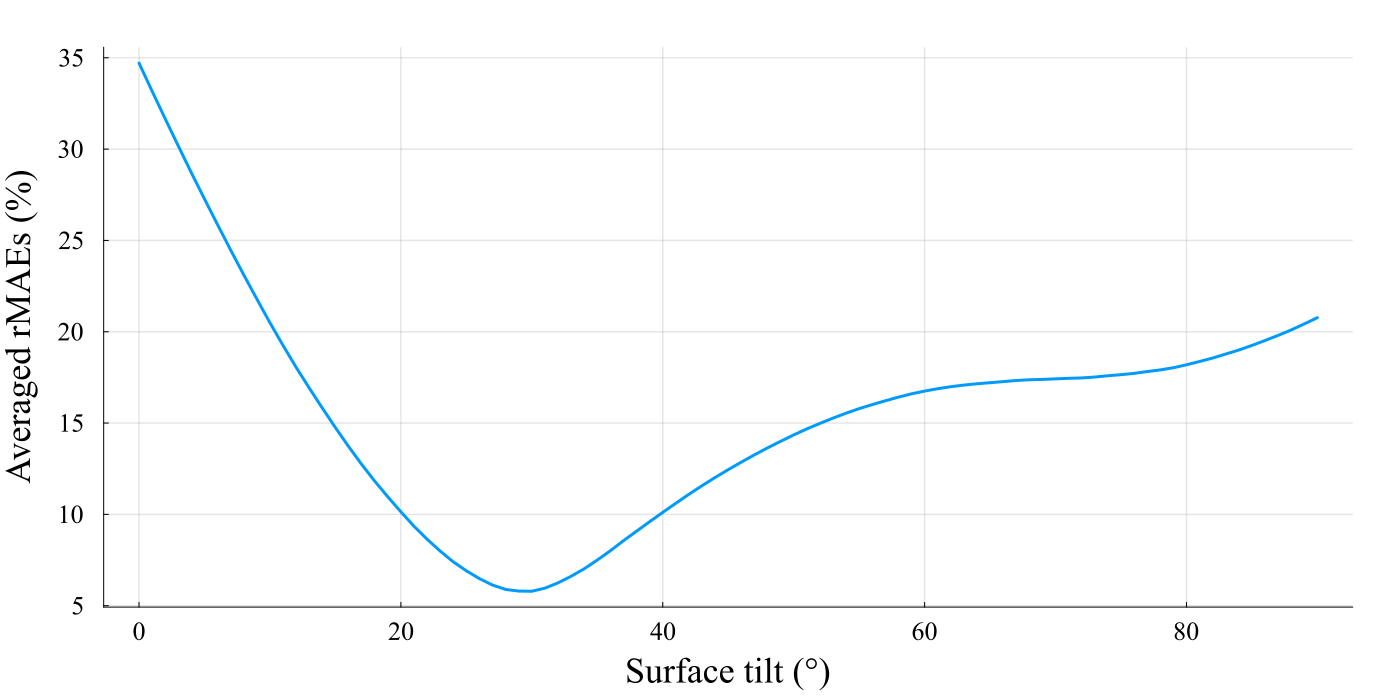
\includegraphics[scale=0.3075]{Surfclub_surface_tilt_and_average_rMAE.png}
    \caption{\small Averaged relative mean absolute errors for clear sky days and no shading with varying surface tilt.}
    \label{Surfclub_surface_tilt_and_average_rMAE.png}
\end{figure}

\begin{figure}
    \centering
    \subfloat[\centering][05/24/2024]{{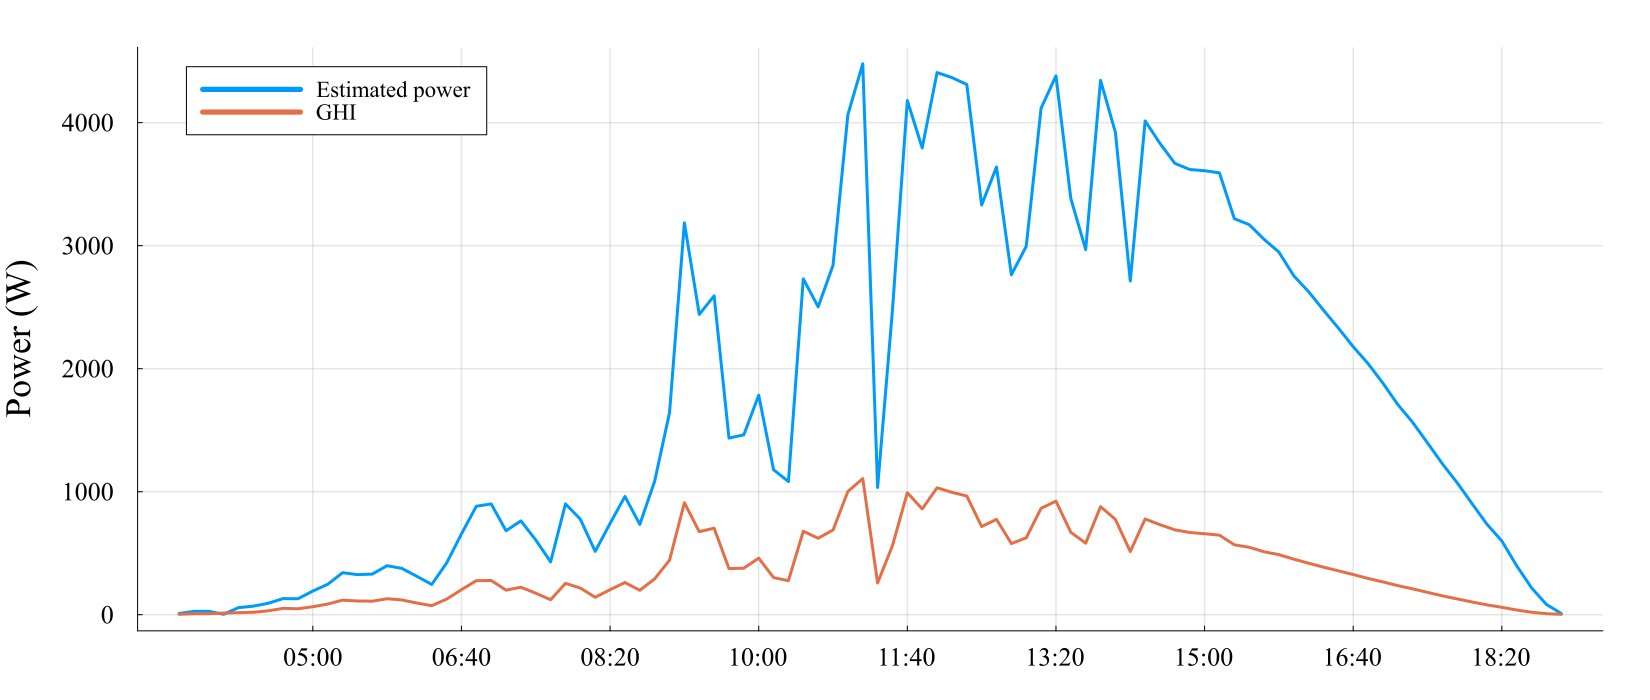
\includegraphics[scale=0.255]{Surfclub_estimated_power_vs_GHI_2024_05_24.png}}} \\
    \subfloat[\centering][07/02/2024]{{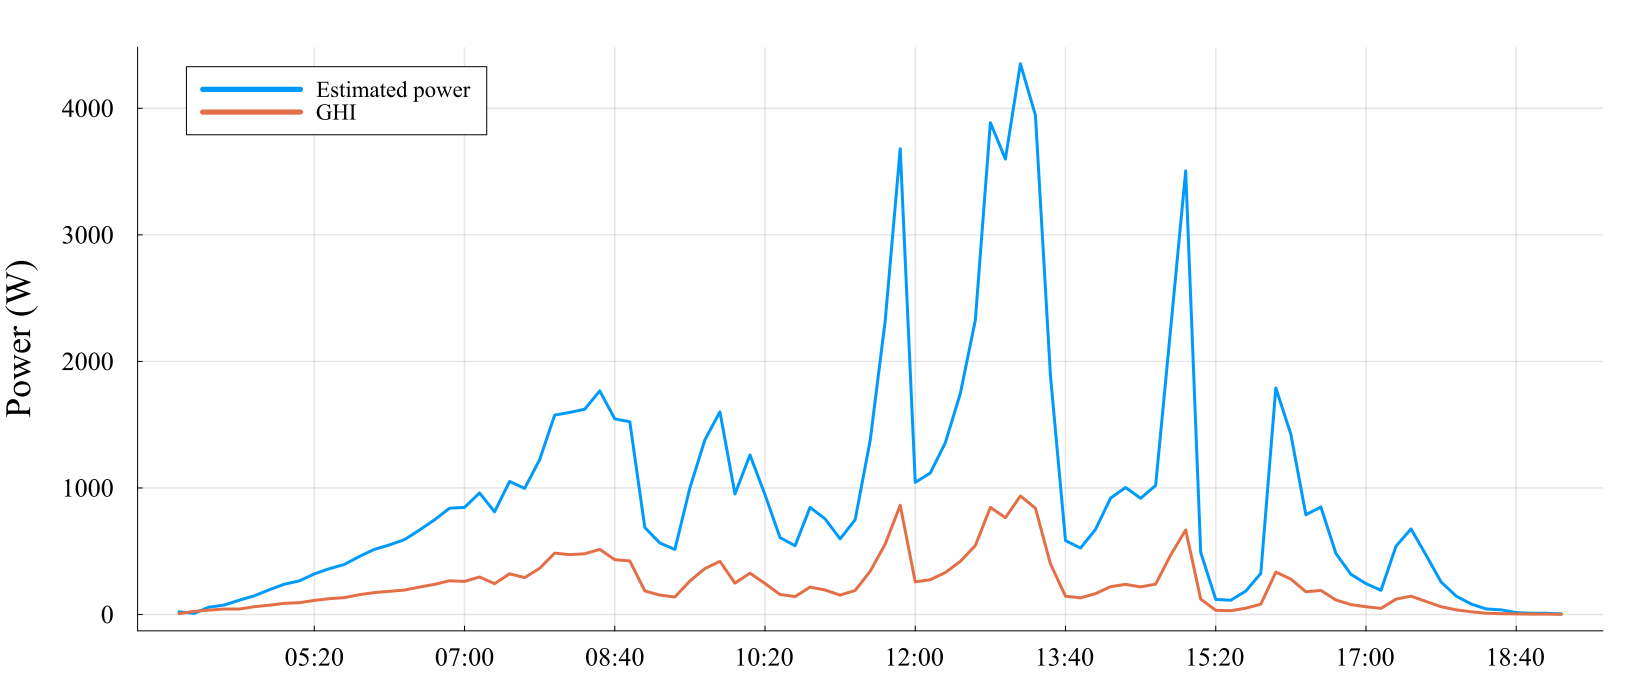
\includegraphics[scale=0.255]{Surfclub_estimated_power_vs_GHI_2024_07_02.png}}} \\
    \subfloat[\centering][10/08/2024]{{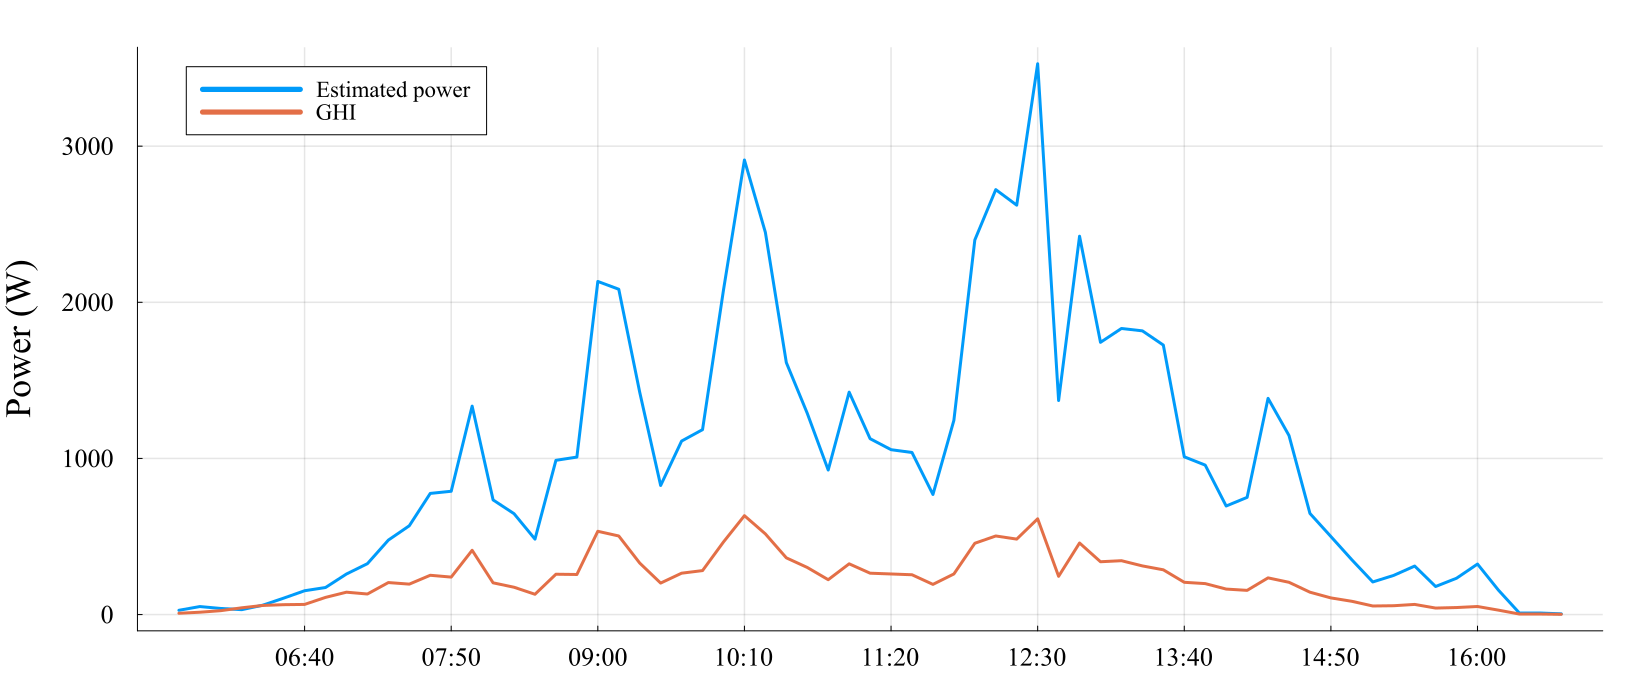
\includegraphics[scale=0.255]{Surfclub_estimated_power_vs_GHI_2024_10_08.png}}}
    \caption{\small Estimated power output of the model and measured global horizontal irradiance for different days of the year.}
    \label{fig:Surfclub_estimated_power_vs_GHI_collection}
\end{figure}

\begin{figure}
    \centering
    \subfloat[\centering][05/24/2024]{{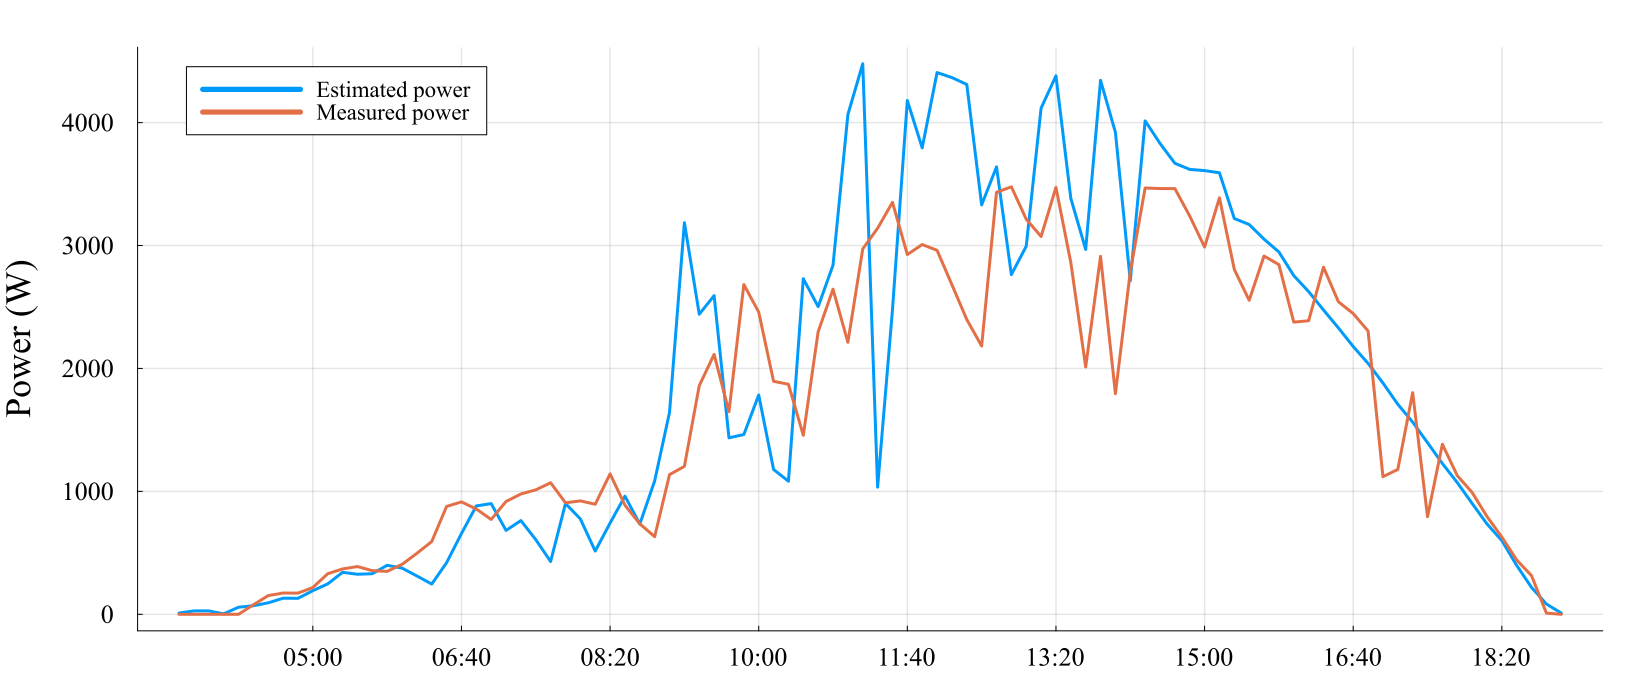
\includegraphics[scale=0.255]{Surfclub_estimated_power_vs_measured_2024_05_24.png}}} \\
    \subfloat[\centering][07/02/2024]{{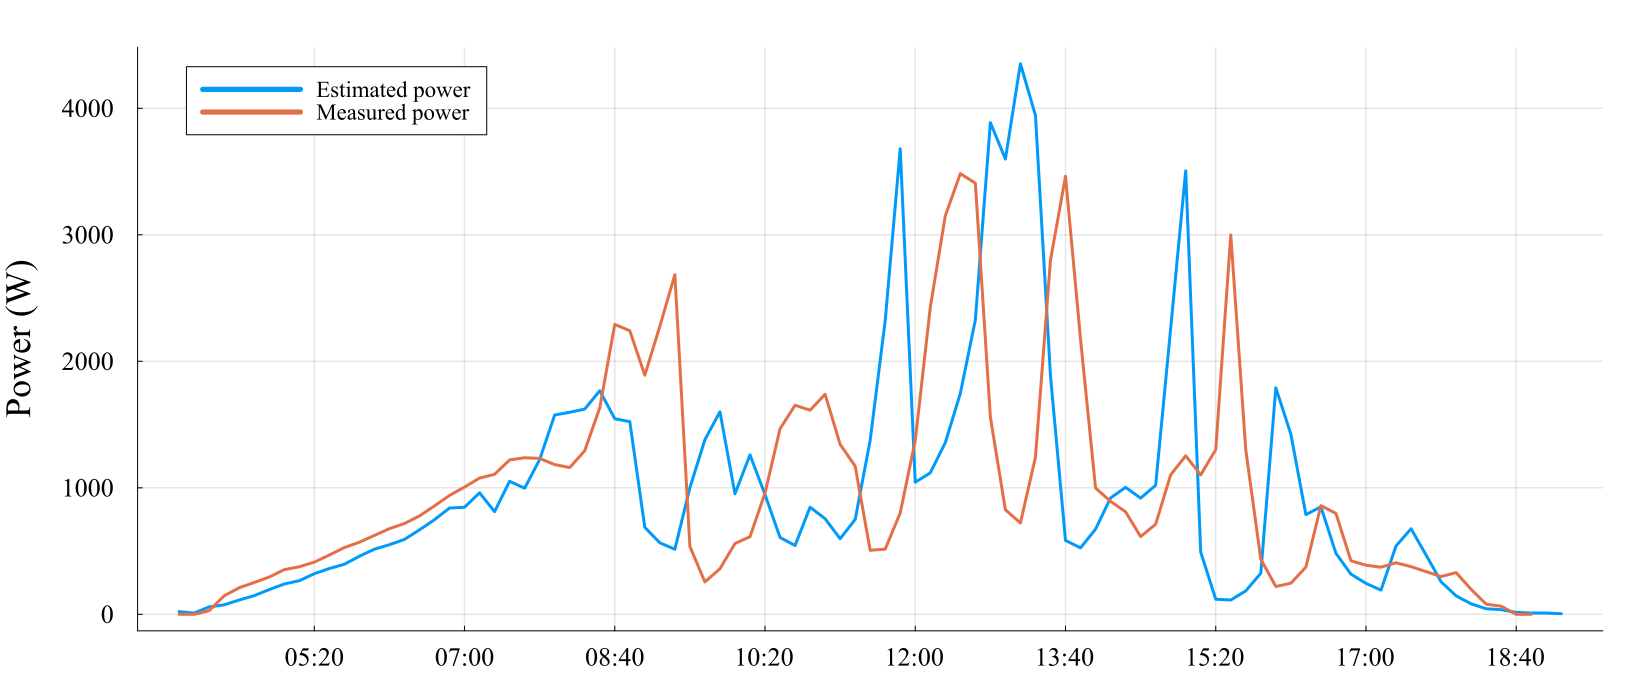
\includegraphics[scale=0.255]{Surfclub_estimated_power_vs_measured_2024_07_02.png}}} \\
    \subfloat[\centering][10/08/2024]{{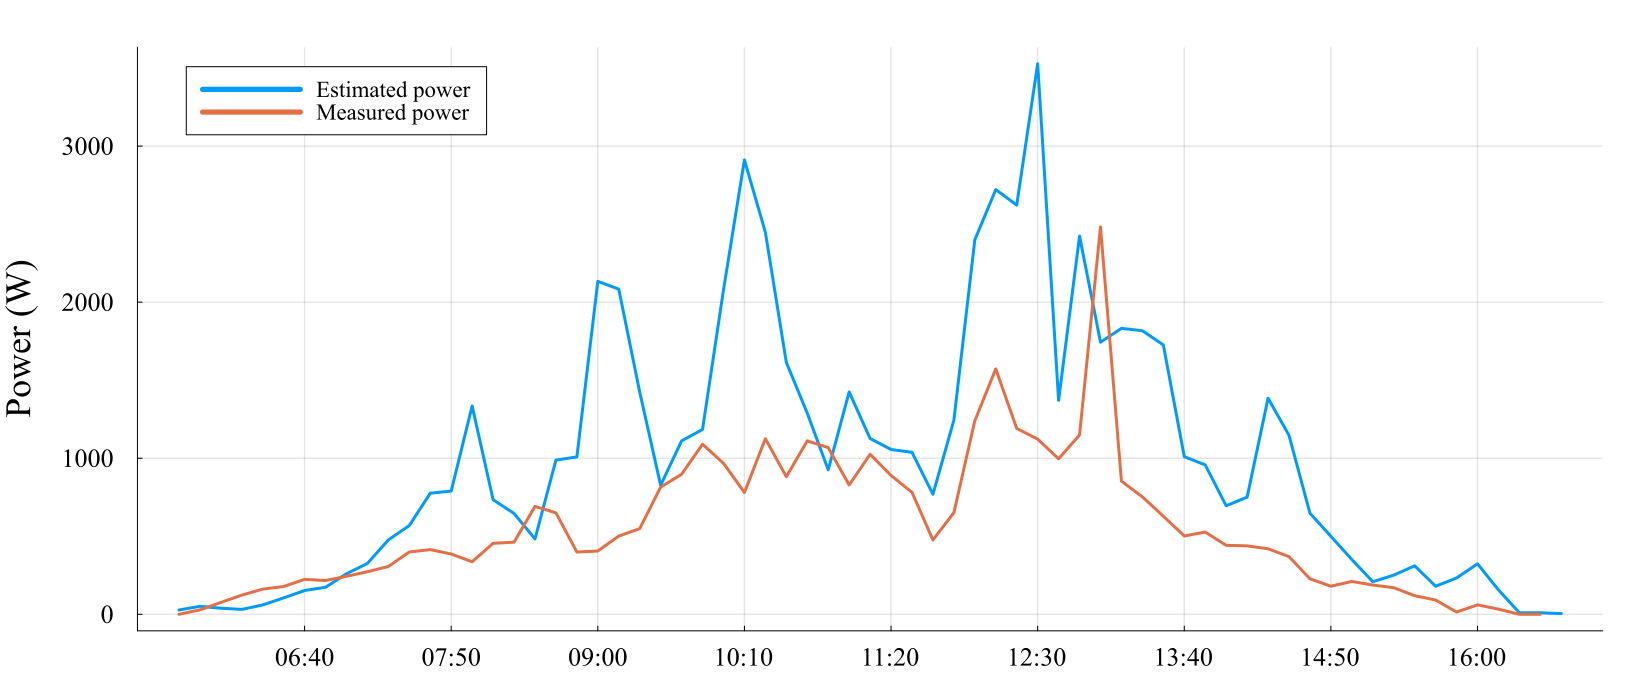
\includegraphics[scale=0.255]{Surfclub_estimated_power_vs_measured_2024_10_08.png}}}
    \caption{\small Estimated power output of the model and measured power output for different days of the year.}
    \label{fig:Surfclub_estimated_power_vs_measured_collection}
\end{figure}

\newpage

\section{Conclusion}
\label{sec:Conclusion}
In this thesis, an approach to model the direct current (DC) power
output of a photovoltaic (PV) system was presented. The core of
the model is based on a well-known single-diode five-parameter
model that can be calibrated with a minimal set of data provided
by manufacturers. The calibration method allows for the determination
of the electrical parameters of a PV panel and the assessment of
the power generated under any conditions of operating temperature
and solar irradiance. This approach was extended to arbitrarily
configured and sized PV systems, taking into account practical
aspects of PV system design. Furthermore, all equations and calculations
involved in the model parameter determination process were presented
in a way that allows the model to be applied effectively to various
types of PV systems. The application of the model requires the
preliminary estimation of the operating conditions. To this end,
well-known thermal and transposition models were introduced,
capable of estimating the operating conditions from meteorological
data, including temperature, wind speed, air pressure, and global
and diffuse horizontal irradiance. The fundamentals related to
solar geometry and solar radiation modeling were introduced to
the extent necessary to understand the individual components of
the presented procedure.

The model was applied to a real-world PV system, and its performance
was evaluated over 154 days within a period of 166 days. The results
suggest that the model's accuracy is highly dependent on the quality
of the input data. The reliability of the model was confirmed during
time periods when the quality of the input data was expected to be
high, specifically, during clear-sky days when the PV system was
not shaded. These time periods were also used to estimate the PV
array's tilt angle, a required model parameter that may be unknown
in real-world applications, with a precision of 2 degrees. Conversely,
it was observed that lower-quality input data inevitably resulted in
reduced accuracy of the model's predictions. In the considered case,
the frequent presence of clouds during the evaluation period, combined
with the distance between the PV system and the irradiance measurement
instrument, as well as shading of the PV system by large trees during
the morning hours, contributed to discrepancies between the measured
and actual meteorological conditions, resulting in lower accuracy of
the model's predictions.

In conclusion, this thesis provided a comprehensive overview of
physical PV system modeling. The presented model can be successfully
used for energy assessments of PV systems that are exposed to stable
and primarily sunny weather conditions without shading obstructions.
Future work could focus on integrating shading analysis and higher-quality
environmental data to enhance the model's predictive capabilities. By
addressing the challenges associated with input data quality and
environmental factors, this thesis contributes valuable insights
to the field of solar energy modeling and aids in the optimization
and planning of PV installations.

\newpage

{\footnotesize\listoffigures}
\newpage

{\footnotesize\listoftables}
\newpage

% Define group titles using \nomgroup
\renewcommand{\nomgroup}[1]{%
  \ifthenelse{\equal{#1}{A}}{\item[\textbf{Solar Angles and Surface Orientation}]}{%
  \ifthenelse{\equal{#1}{B}}{\item[\textbf{Irradiance Components}]}{%
  \ifthenelse{\equal{#1}{C}}{\item[\textbf{Transposition Factors}]}{%
  \ifthenelse{\equal{#1}{D}}{\item[\textbf{Thermal Model Parameters}]}{%
  \ifthenelse{\equal{#1}{E}}{\item[\textbf{Cell Temperature and Irradiance Ratios}]}{%
  \ifthenelse{\equal{#1}{F}}{\item[\textbf{Electrical Parameters}]}{%
  \ifthenelse{\equal{#1}{G}}{\item[\textbf{Reference Conditions}]}{%
  \ifthenelse{\equal{#1}{H}}{\item[\textbf{Model Parameters}]}{%
  \ifthenelse{\equal{#1}{I}}{\item[\textbf{Temperature Coefficients}]}{%
  \ifthenelse{\equal{#1}{J}}{\item[\textbf{Constants and Physical Quantities}]}{%
  \ifthenelse{\equal{#1}{K}}{\item[\textbf{Array Configuration Parameters}]}{}}}}}}}}}}}}

% Nomenclature entries with group identifiers

% Solar Angles and Surface Orientation (Group A)
\nomenclature[A]{\(\alpha_{\text{s}}\)}{Solar azimuth angle (°)}
\nomenclature[A]{\(\gamma_{\text{s}}\)}{Solar altitude angle (°)}
\nomenclature[A]{\(\psi_{\text{s}}\)}{Solar zenith angle (°)}
\nomenclature[A]{\(\alpha\)}{Surface azimuth angle (°)}
\nomenclature[A]{\(\beta\)}{Surface tilt angle (°)}
\nomenclature[A]{\(\nu\)}{Surface incidence angle (°)}

% Irradiance Components (Group B)
\nomenclature[B]{\(G_{\text{h}}\)}{Global horizontal irradiance (\si{\watt\per\meter\squared})}
\nomenclature[B]{\(B_{\text{h}}\)}{Beam horizontal irradiance (\si{\watt\per\meter\squared})}
\nomenclature[B]{\(D_{\text{h}}\)}{Diffuse horizontal irradiance (\si{\watt\per\meter\squared})}
\nomenclature[B]{\(G_{\text{c}}\)}{Global in-plane irradiance (\si{\watt\per\meter\squared})}
\nomenclature[B]{\(B_{\text{c}}\)}{Beam component of in-plane irradiance (\si{\watt\per\meter\squared})}
\nomenclature[B]{\(D_{\text{c}}\)}{Diffuse component of in-plane irradiance (\si{\watt\per\meter\squared})}
\nomenclature[B]{\(R_{\text{c}}\)}{Reflected component of in-plane irradiance (\si{\watt\per\meter\squared})}

% Transposition Factors (Group C)
\nomenclature[C]{\(\tau_{D}\)}{Transposition factor for diffuse irradiance (-)}
\nomenclature[C]{\(\tau_{R}\)}{Transposition factor for ground-reflected irradiance (-)}

% Thermal Model Parameters (Group D)
\nomenclature[D]{\(T_{\text{noct}}\)}{Nominal Operating Cell Temperature (\si{\degreeCelsius})}
\nomenclature[D]{\(WS\)}{Wind speed (\si{\meter\per\second})}
\nomenclature[D]{\(T_{\text{m}}\)}{Back-surface module temperature (\si{\kelvin})}
\nomenclature[D]{\(a\)}{Empirically determined coefficient in Sandia's thermal model (-)}
\nomenclature[D]{\(b\)}{Empirically determined coefficient in Sandia's thermal model (-)}

% Cell Temperature and Irradiance Ratios (Group E)
\nomenclature[E]{\(T\)}{Cell temperature (\si{\kelvin})}
\nomenclature[E]{\(\alpha_{\text{G}}\)}{Ratio of global in-plane irradiance to irradiance at STC (-)}

% Electrical Parameters (Group F)
\nomenclature[F]{\(I\)}{Current generated by the panel (\si{\ampere})}
\nomenclature[F]{\(V\)}{Voltage generated by the panel (\si{\volt})}
\nomenclature[F]{\(I_{\text{sc}}\)}{Short-circuit current (\si{\ampere})}
\nomenclature[F]{\(V_{\text{oc}}\)}{Open-circuit voltage (\si{\volt})}
\nomenclature[F]{\(I_{\text{mp}}\)}{Current at the maximum power point (\si{\ampere})}
\nomenclature[F]{\(V_{\text{mp}}\)}{Voltage at the maximum power point (\si{\volt})}
\nomenclature[F]{\(P_{\text{mp}}\)}{Maximum power output (\si{\watt})}

% Reference Conditions (Group G)
\nomenclature[G]{\(T_{\text{ref}}\)}{Reference temperature at STC (\SI{298.15}{\kelvin})}
\nomenclature[G]{\(G_{\text{ref}}\)}{Reference irradiance at STC (\SI{1000}{\watt\per\meter\squared})}
\nomenclature[G]{ref}{Subscript referring to the parameter at reference conditions STC}

% Model Parameters (Group H)
\nomenclature[H]{\(I_{\text{L}}\)}{Photocurrent or light-generated current (\si{\ampere})}
\nomenclature[H]{\(I_{0}\)}{Reverse saturation current (\si{\ampere})}
\nomenclature[H]{\(n\)}{Diode ideality factor (-)}
\nomenclature[H]{\(R_{\text{s}}\)}{Series resistance (\si{\ohm})}
\nomenclature[H]{\(R_{\text{sh}}\)}{Shunt (parallel) resistance (\si{\ohm})}
\nomenclature[H]{\(K\)}{Thermal correction factor (-)}
\nomenclature[H]{\(R_{\text{so}}\)}{Reciprocal of the slope at the open-circuit point (-)}
\nomenclature[H]{\(R_{\text{sho}}\)}{Reciprocal of the slope at the short-circuit point (-)}

% Temperature Coefficients (Group I)
\nomenclature[I]{\(\mu_{\text{I,sc}}\)}{Short-circuit current temperature coefficient (\si{\ampere\per\kelvin})}
\nomenclature[I]{\(\mu_{\text{V,oc}}\)}{Open-circuit voltage temperature coefficient (\si{\volt\per\kelvin})}
\nomenclature[I]{\(\mu_{P_{\text{mp}}}\)}{Maximum power temperature coefficient (\si{\percent\per\kelvin})}

% Constants and Physical Quantities (Group J)
\nomenclature[J]{\(k\)}{Boltzmann's constant (\SI{1.380649e-23}{\joule\per\kelvin})}
\nomenclature[J]{\(q\)}{Elementary charge (\SI{1.602176634e-19}{\coulomb})}

% Array Configuration Parameters (Group K)
\nomenclature[K]{\(N_{c}\)}{Number of cells connected in series per module (-)}
\nomenclature[K]{\(N_{m}\)}{Number of modules connected in series per string (-)}
\nomenclature[K]{\(N_{s}\)}{Total number of cells connected in series per string (-)}
\nomenclature[K]{\(N_{p}\)}{Number of strings connected in parallel in the array (-)}

\setlength{\nomitemsep}{0.5pt}{\footnotesize\printnomenclature} % nomenclature is only printed with the right build recipe
\newpage

{\footnotesize\bibliography{references}{}\bibliographystyle{plain}}

\end{document}
